\chapter{HASIL DAN PEMBAHASAN}
\label{chap:pengujiananalisis}

Pada bab ini akan dipaparkan hasil pengerjaan tugas akhir berupa \emph{Web NFT Marketplace}, \emph{API}, \emph{Smart Contract}, dan \emph{Metaverse}. 

Hasil penelitian adalah sebagai berikut:

\subsection{\emph{Web NFT Marketplace}}
\label{sec:webnftmarketplace}

\subsection{Halaman Awal \emph{NFT Marketplace}} 

\begin{figure} [H] \centering
  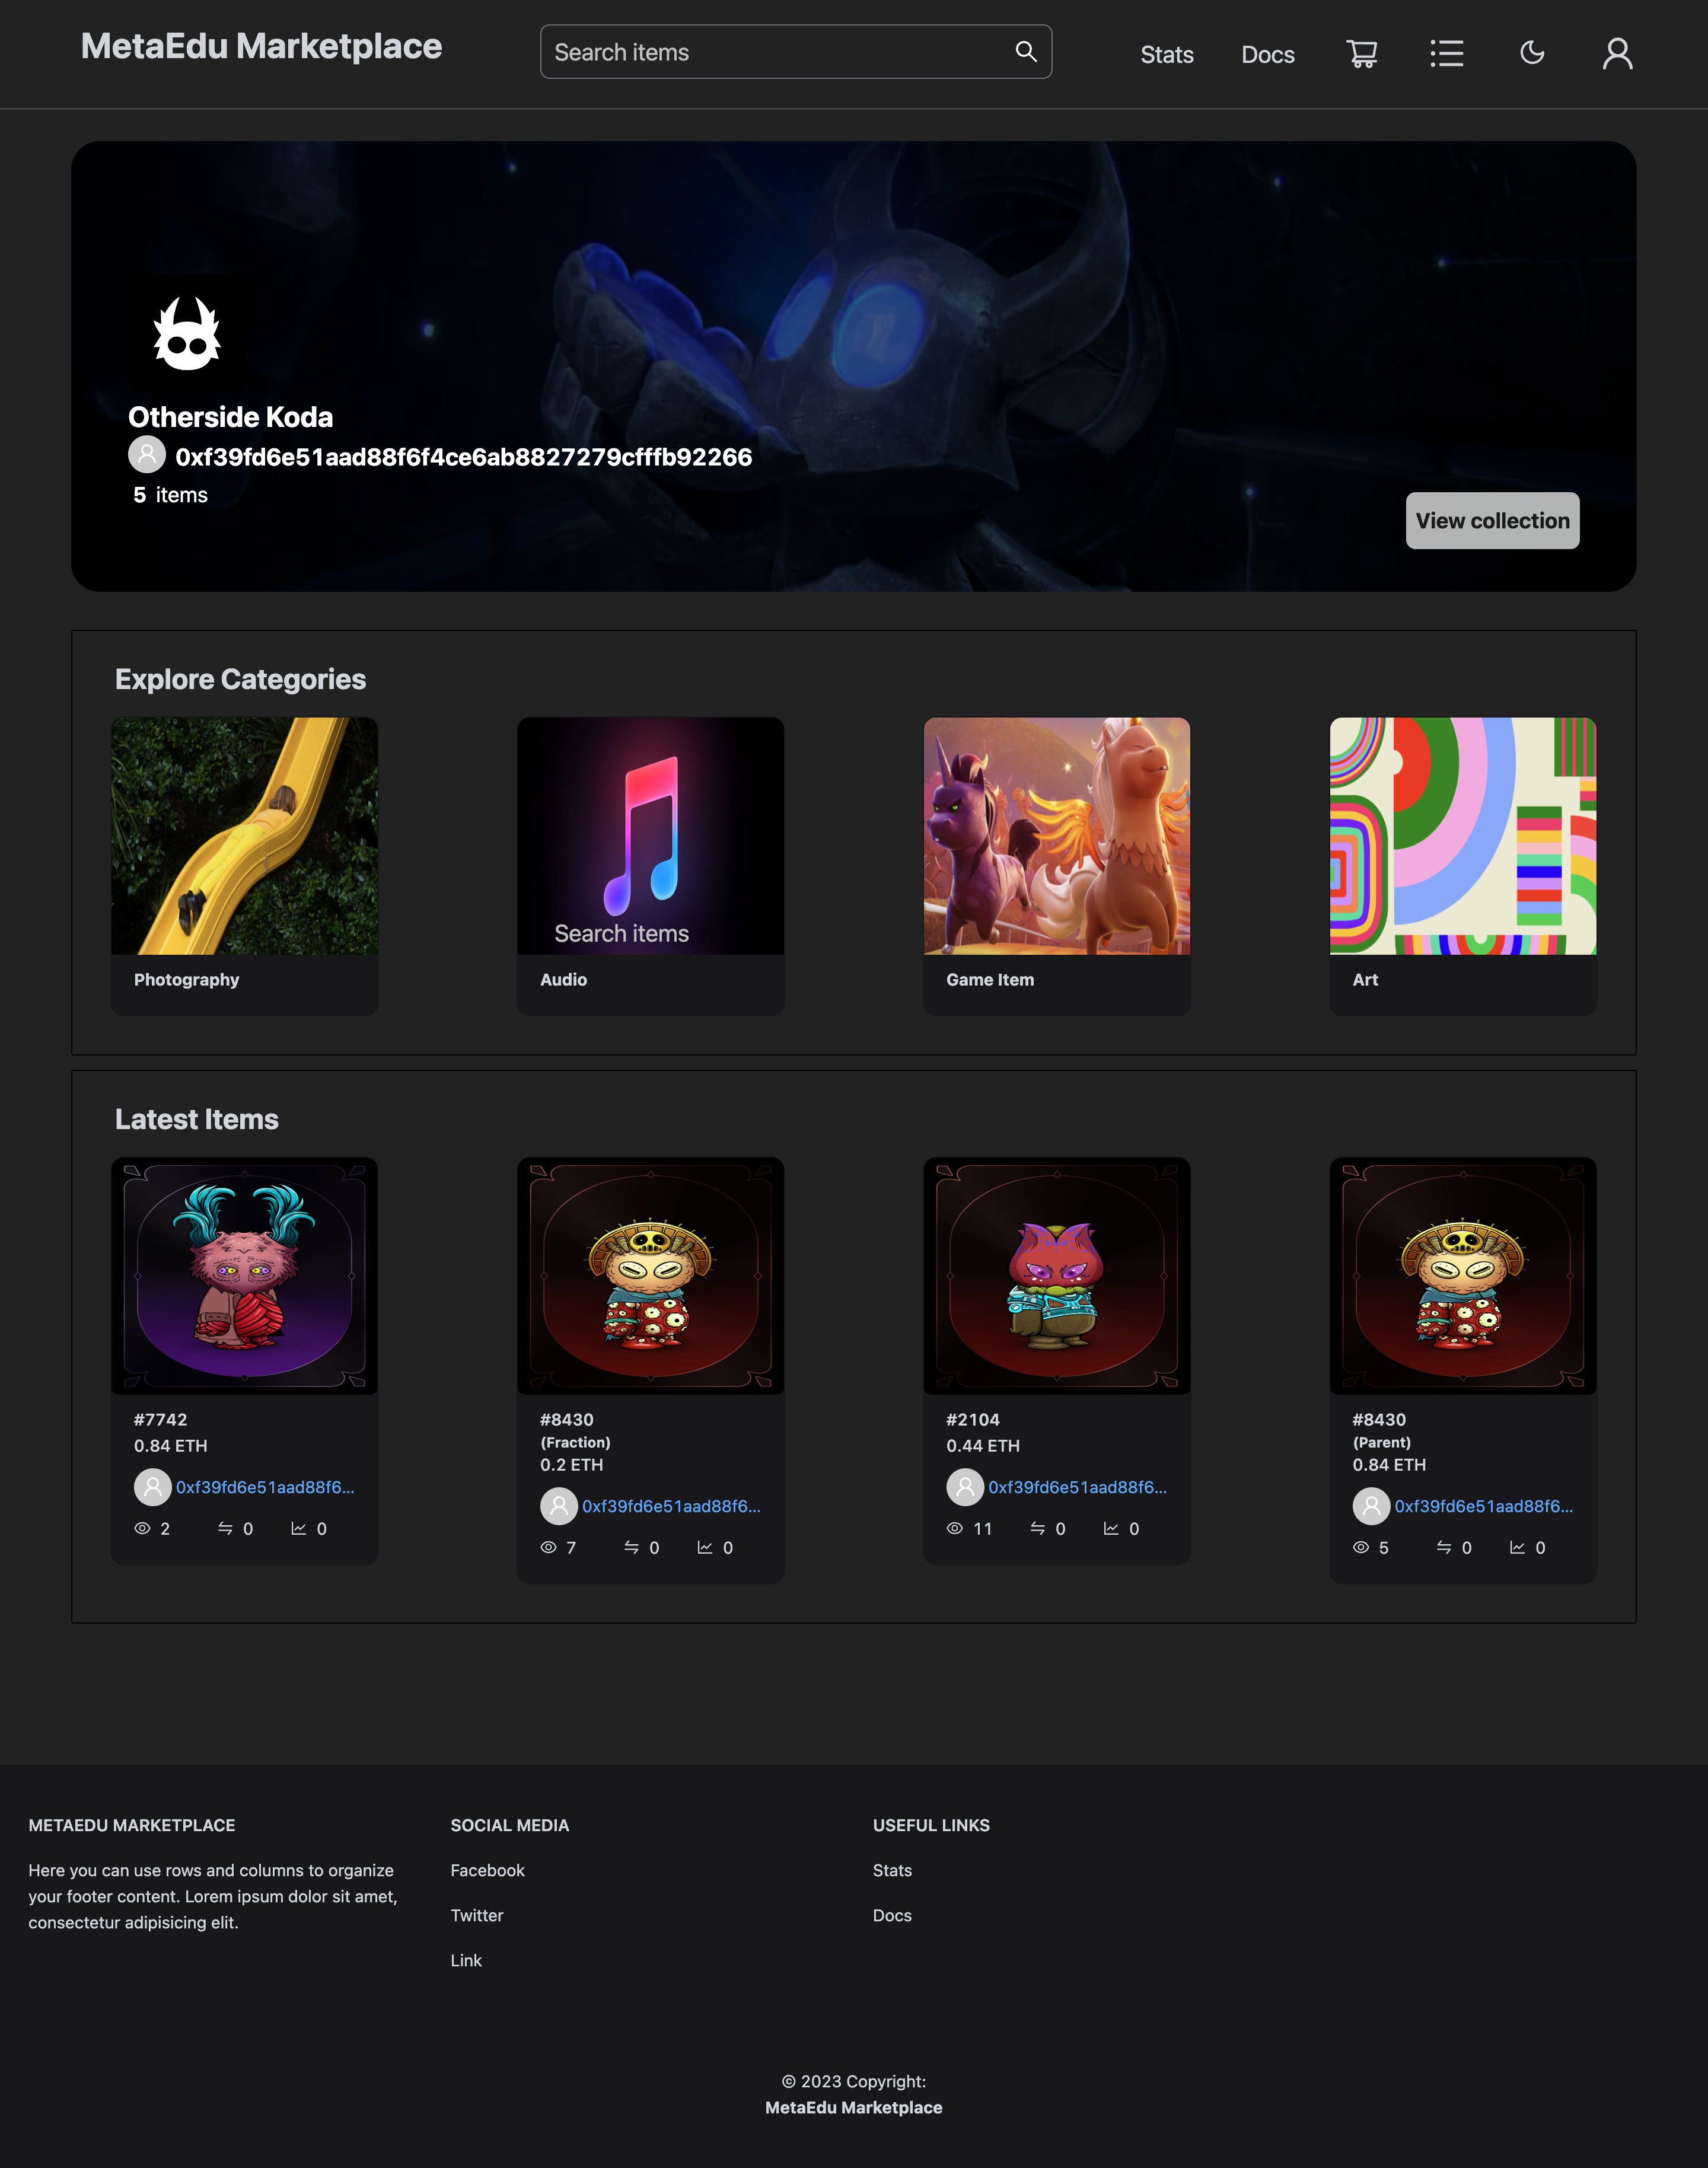
\includegraphics[scale=0.12]{gambar/img-frontend-index.png}
  \caption{Halaman awal \emph{NFT Marketplace}}
  \label{fig:NFTMarketplace}
\end{figure}

Tampilan awal \emph{NFT Marketplace}, menampilkan koleksi \emph{token}, kategori \emph{token}, dan \emph{token} terbaru.

\subsection{Halaman \emph{Minting Token}}

\begin{figure} [H] \centering
  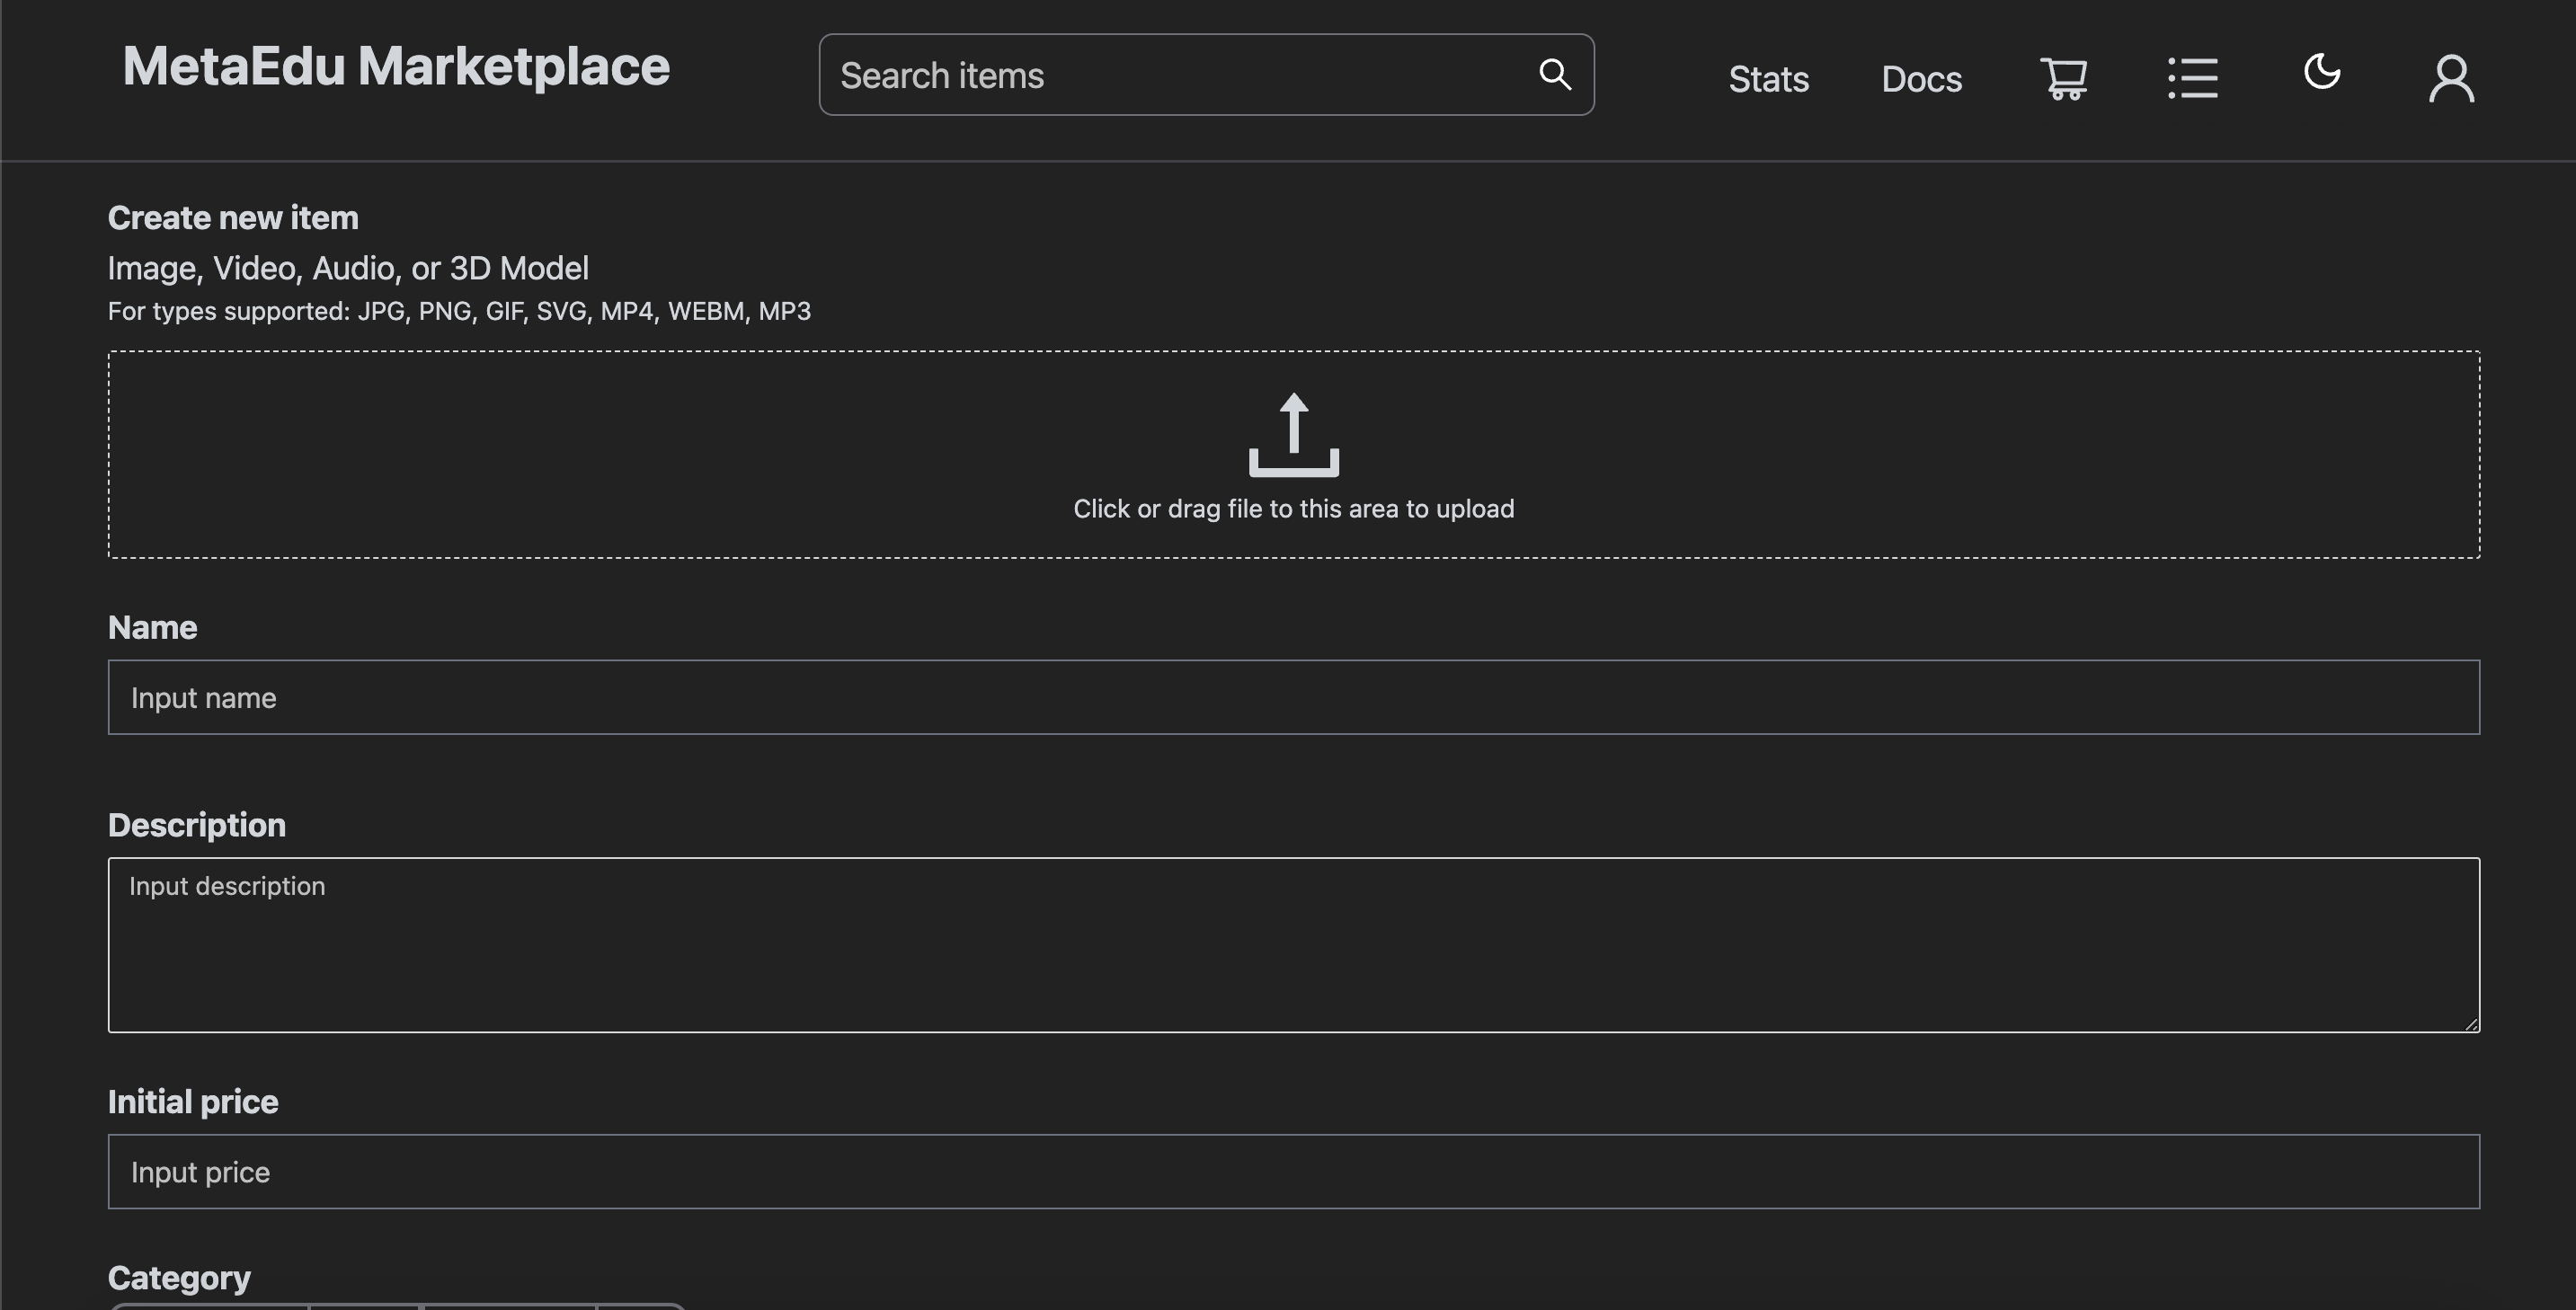
\includegraphics[scale=0.3]{gambar/img-frontend-add-token.png}
  \caption{Halaman \emph{Minting Token}}
  \label{fig:TokenMinting}
\end{figure}

Halaman \emph{Minting token} merupakan halaman yang digunakan \emph{user} untuk membuat \emph{token} baru. Untuk membuat \emph{token} baru, \emph{user} perlu memasukan \emph{image} \emph{token}, nama \emph{token}, harga awal, suplai, dan koleksi. 

\subsection{Halaman Detail \emph{Token}}

\begin{figure} [H] \centering
  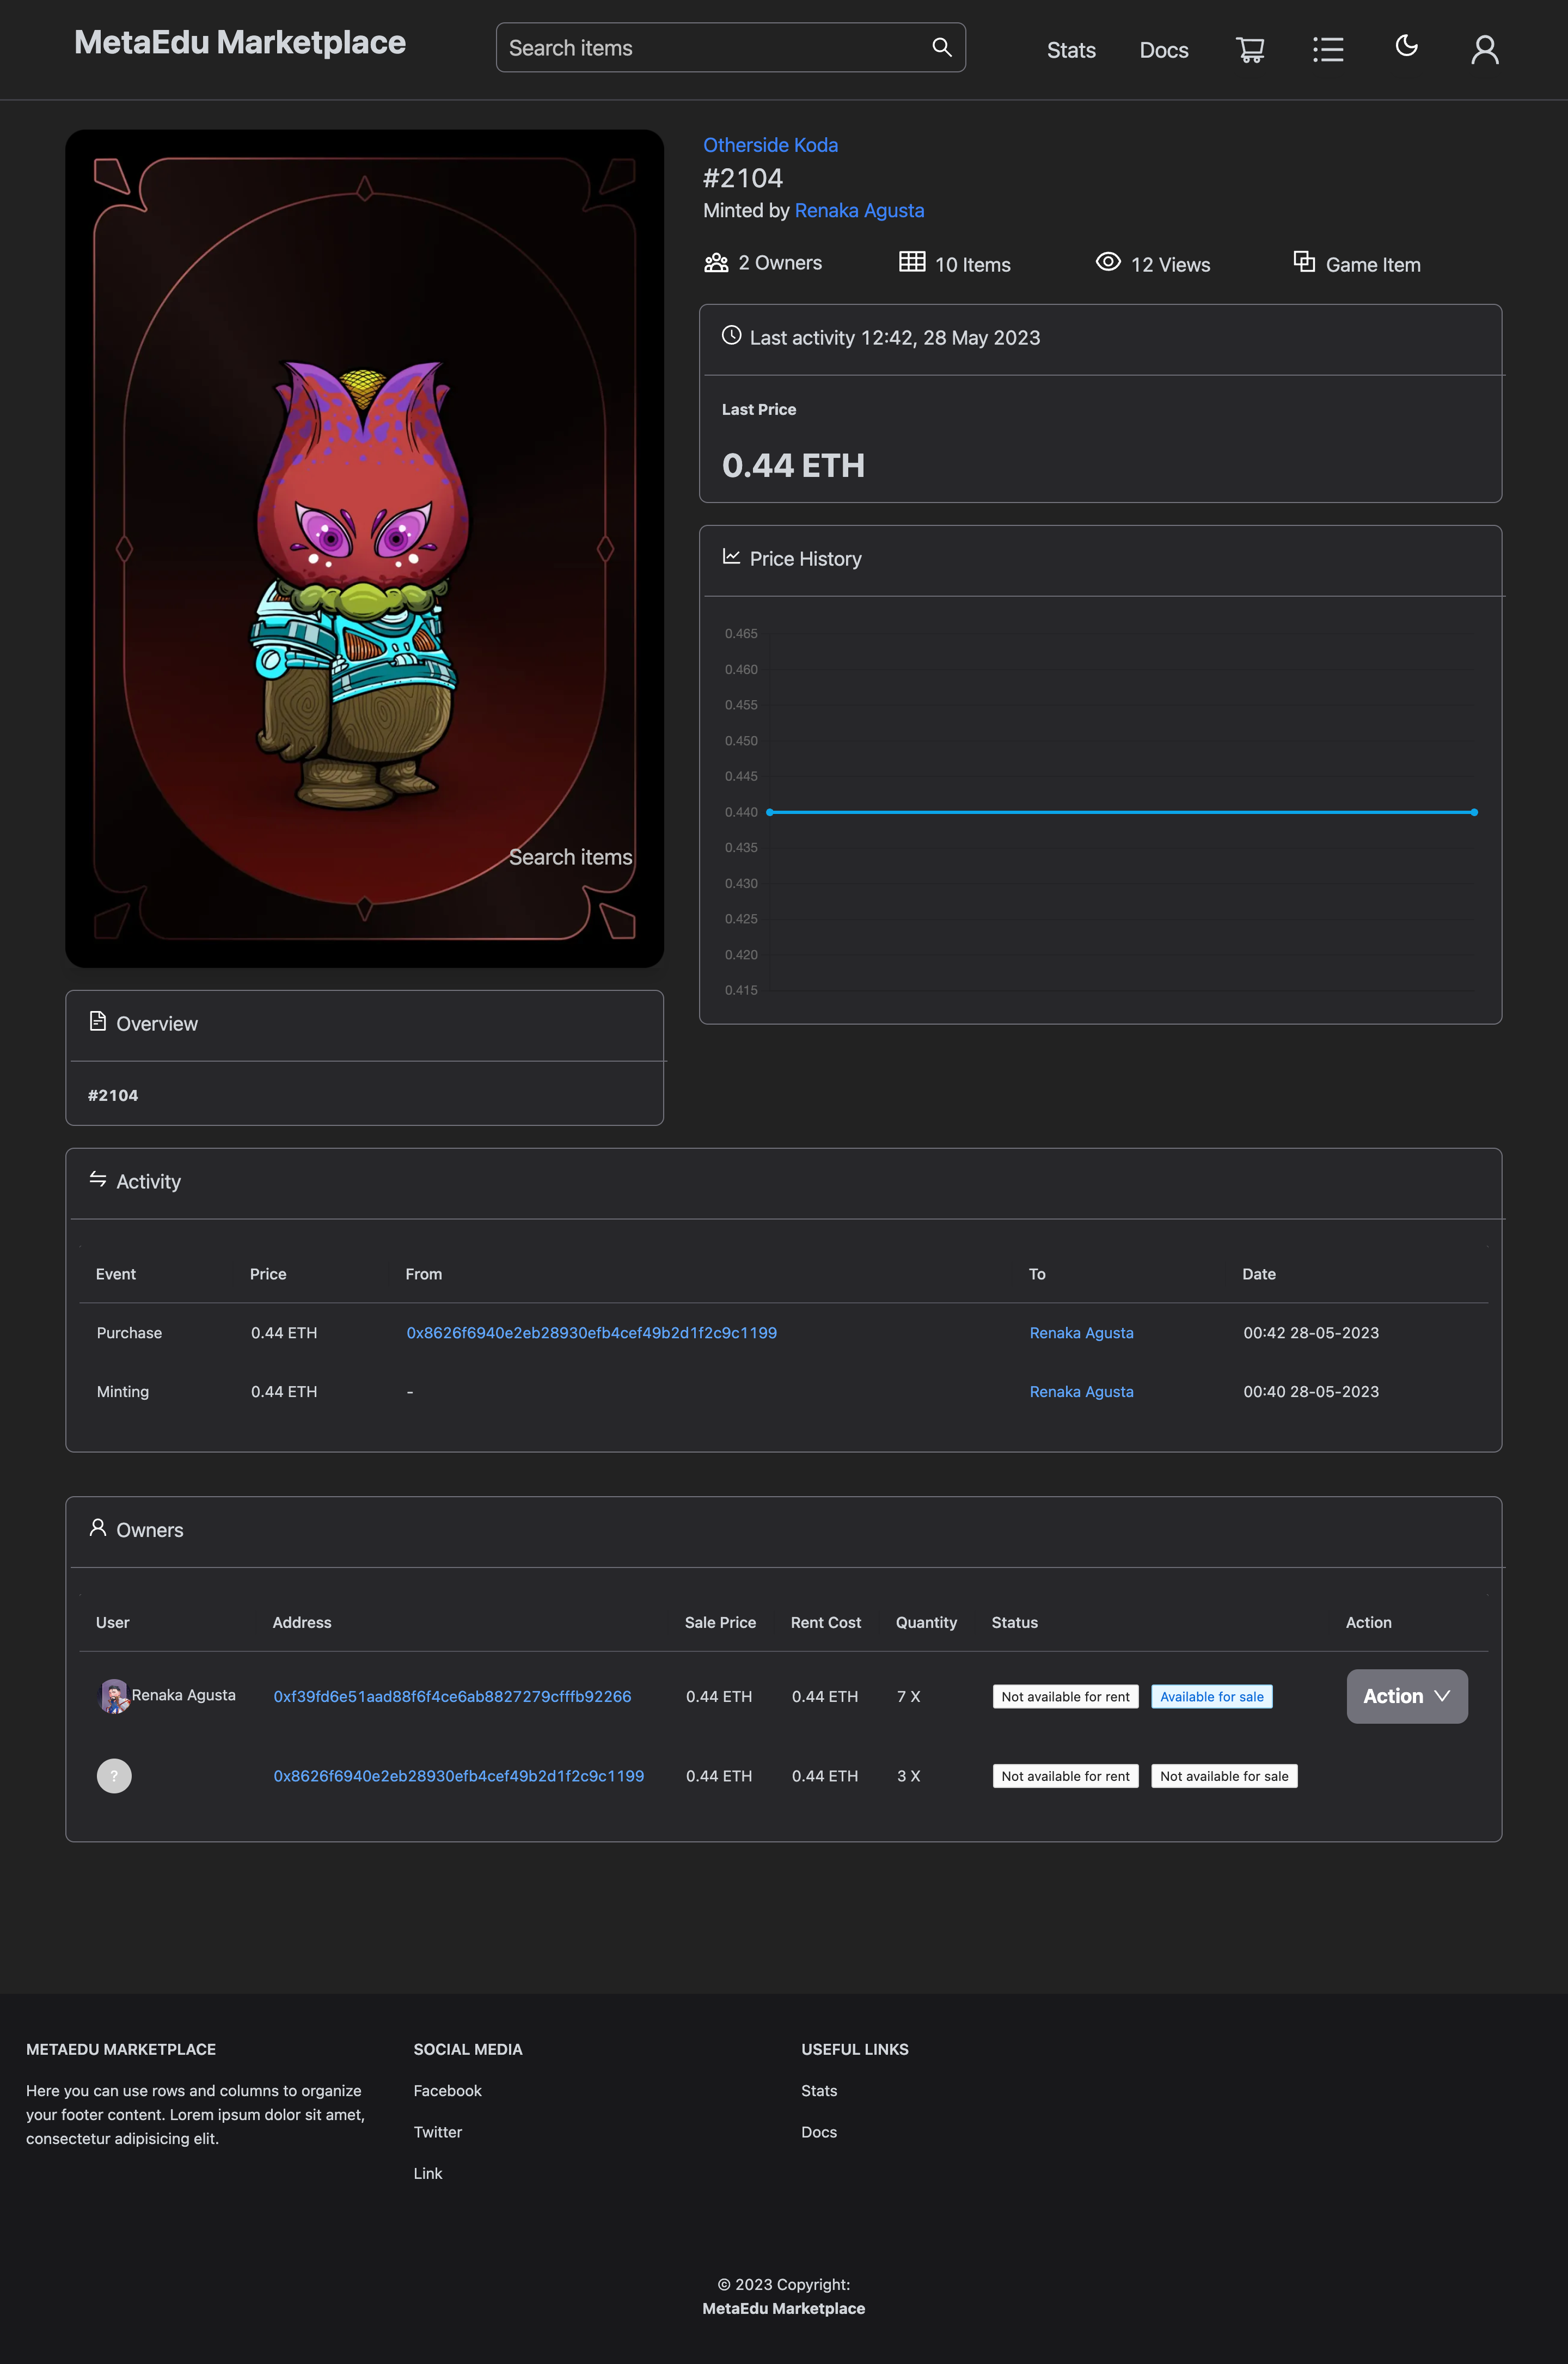
\includegraphics[scale=0.1]{gambar/img-frontend-token-detail.png}
  \caption{Halaman detail \emph{Token}}
  \label{fig:TokenDetail}
\end{figure}

Halaman detail \emph{token} menampilkan informasi-informasi mengenai nama \emph{token}, harga terakhir, pergerakan harga, riwayat transaksi, daftar kepemilkan dan lainnya. 

\subsection{Halaman Pencarian \emph{Token}}
\begin{figure} [H] \centering
  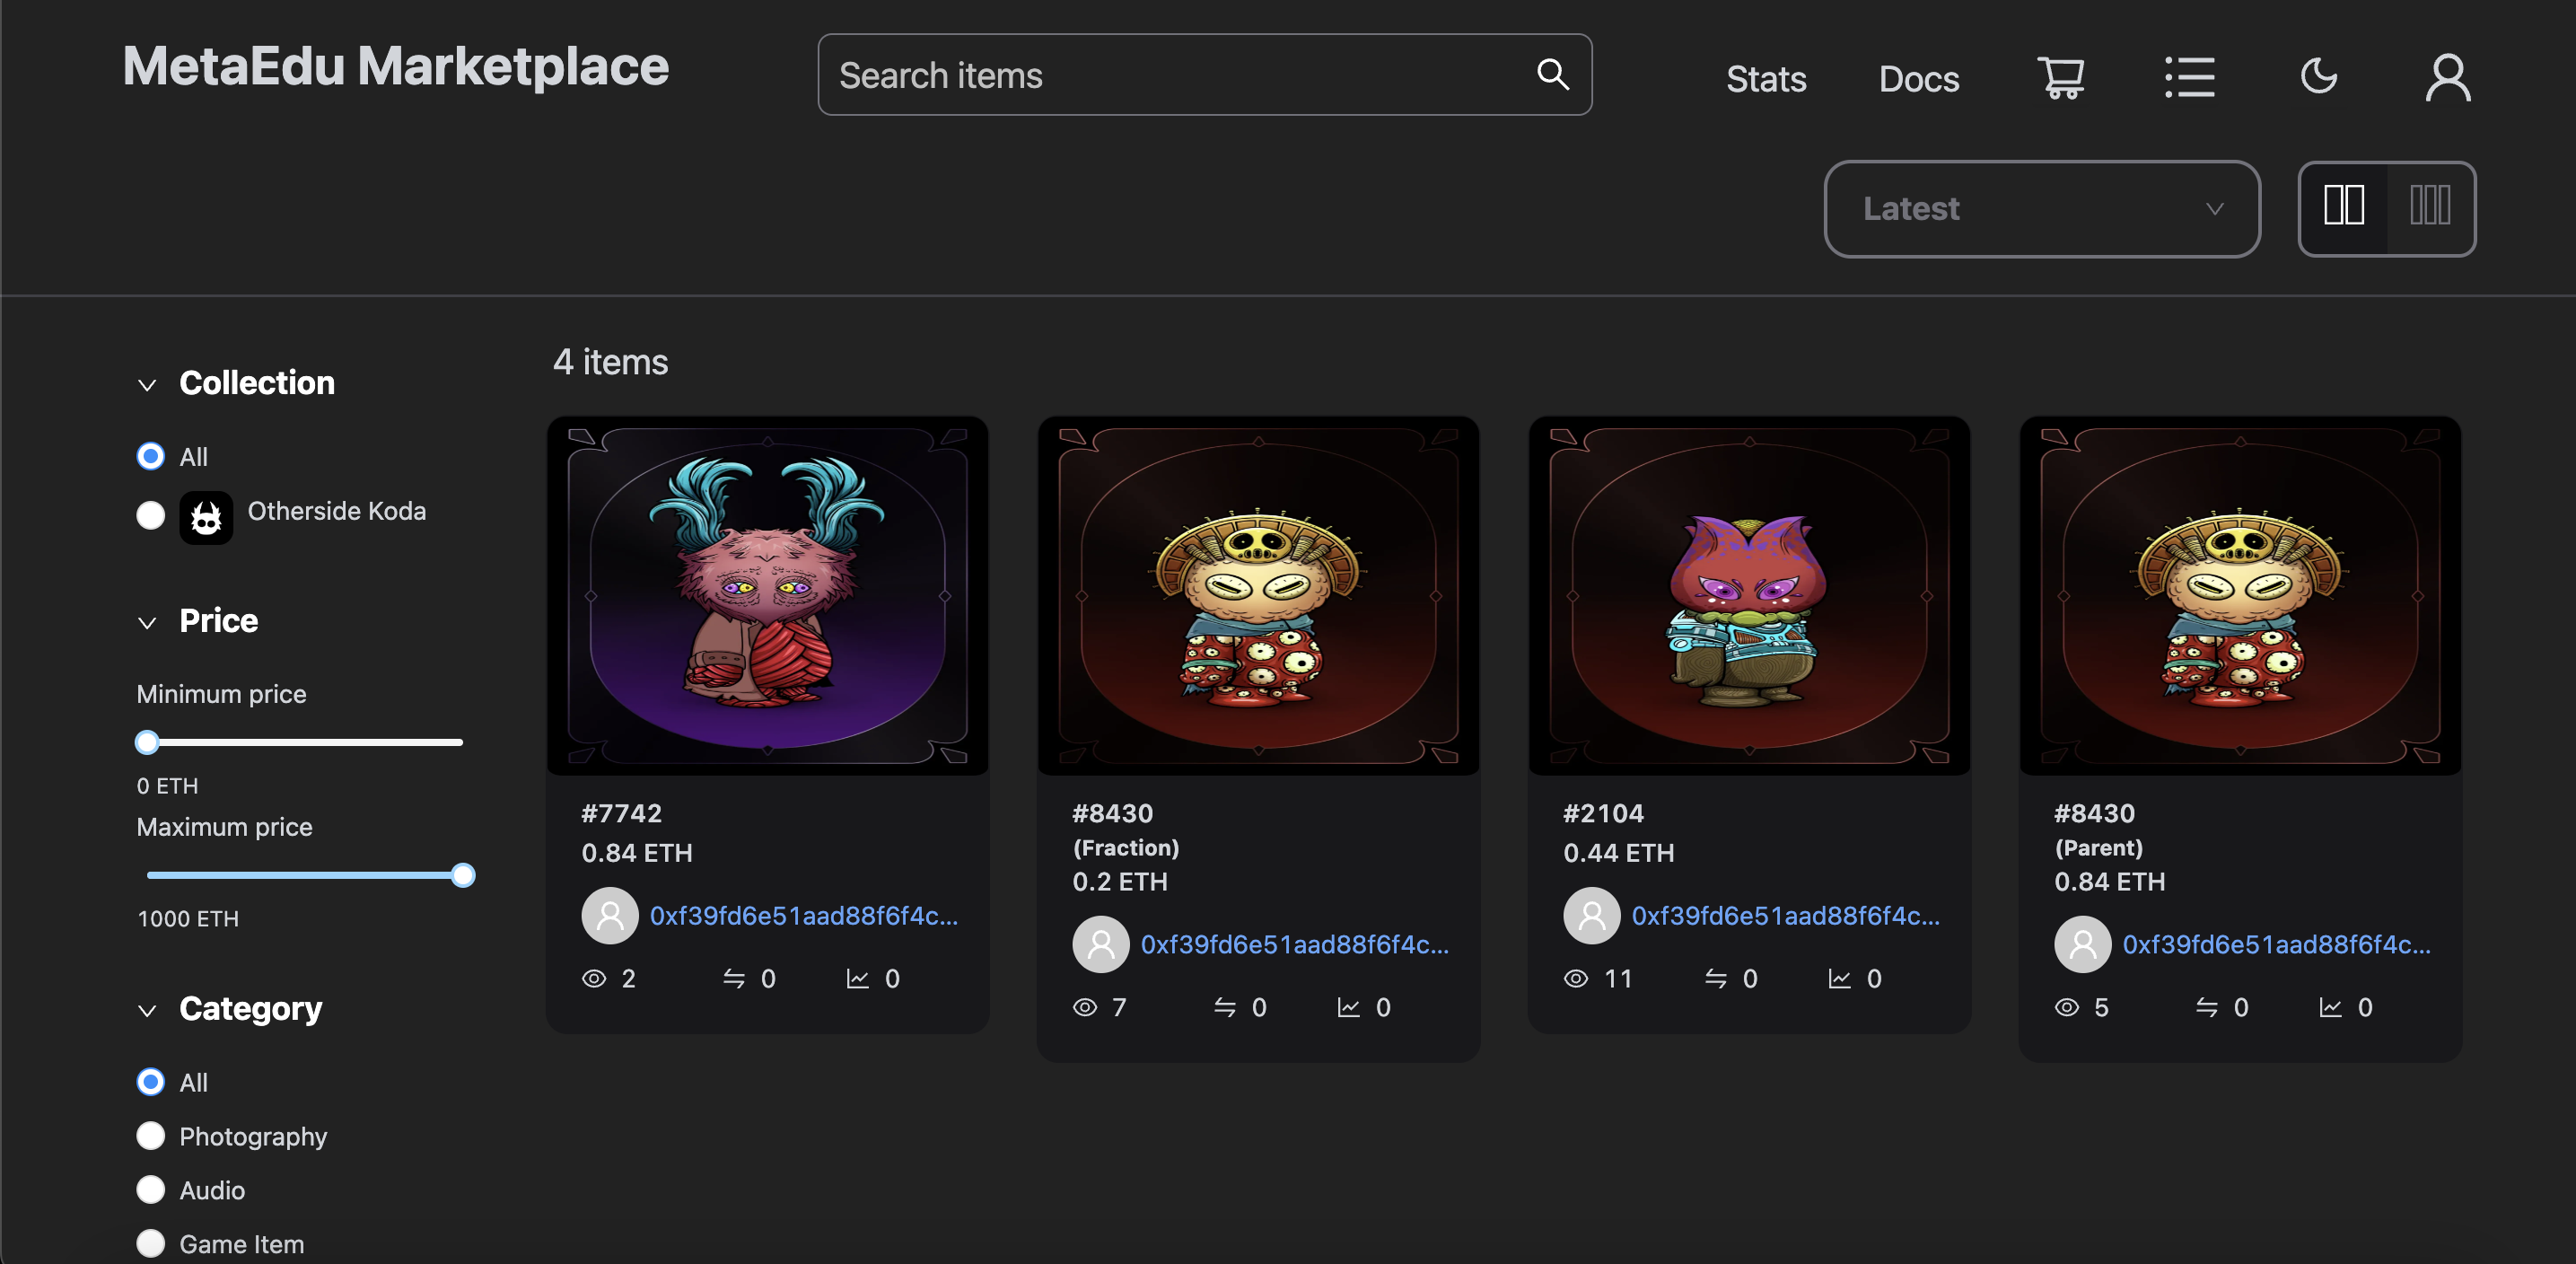
\includegraphics[scale=0.3]{gambar/img-frontend-search.png}
  \caption{Halaman pencarian \emph{Token}}
  \label{fig:TokenSearch}
\end{figure}

Halaman pencarian \emph{token} digunakan oleh \emph{user} untuk mencari \emph{token} tertentu berdasarkan nama, kategori, harga, dan koleksi.

\subsection{Halaman Detail Koleksi}
\begin{figure} [H] \centering
  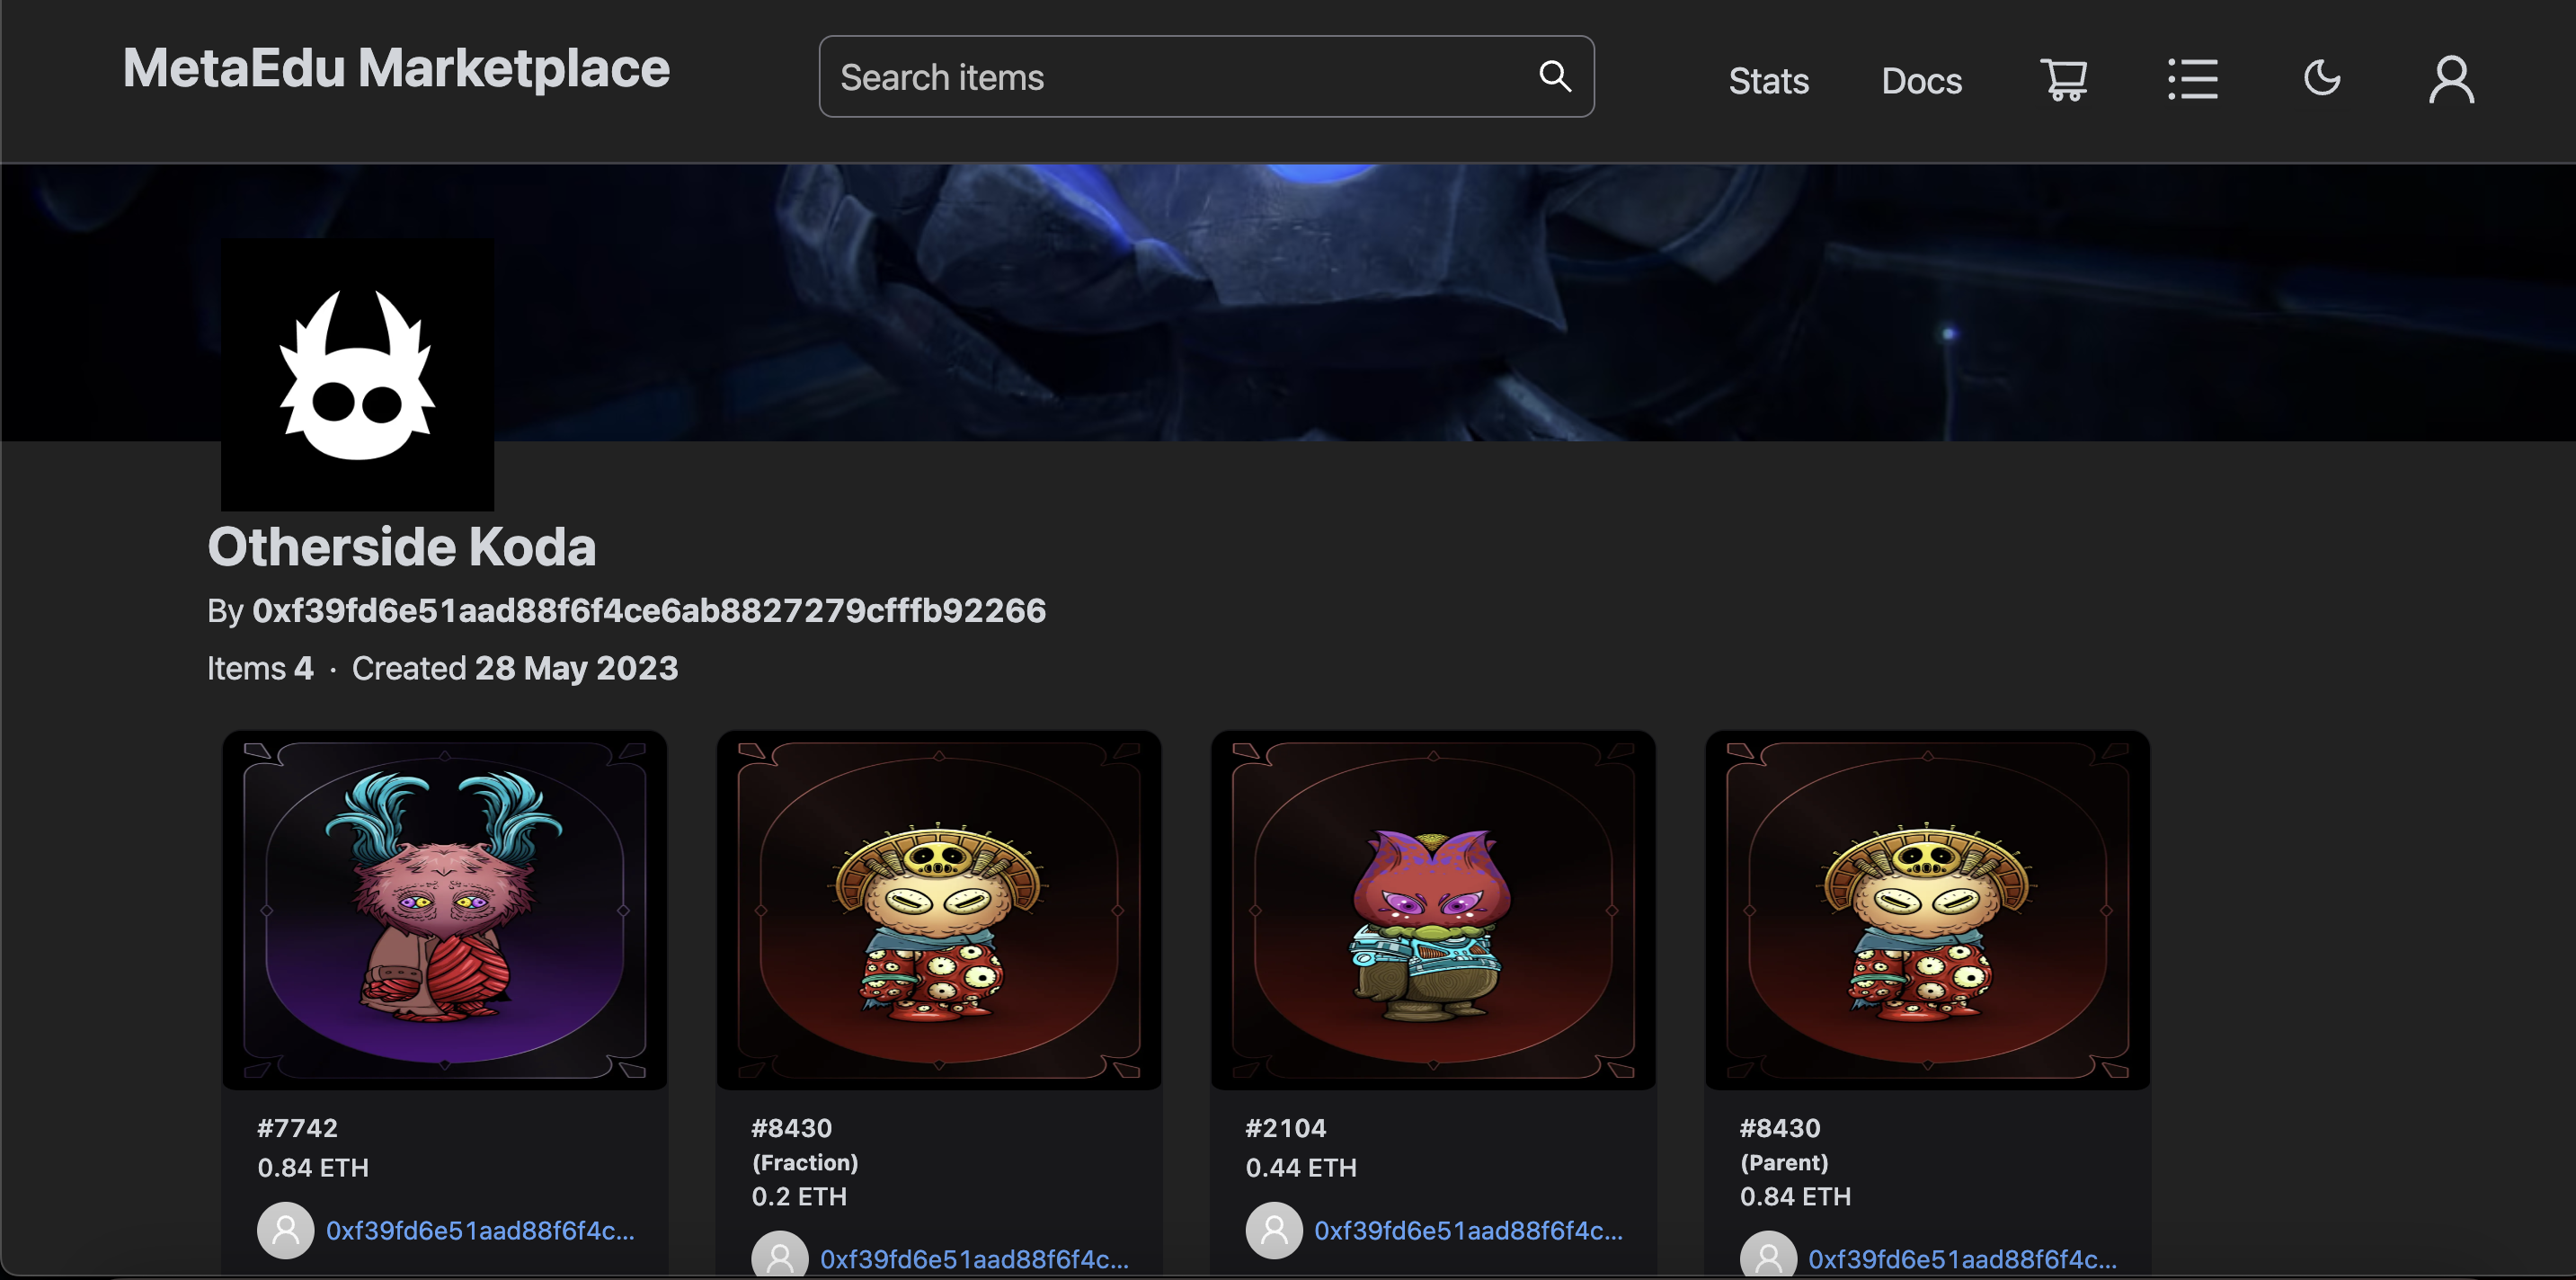
\includegraphics[scale=0.3]{gambar/img-frontend-collection.png}
  \caption{Halaman detail koleksi}
  \label{fig:CollectionDetail}
\end{figure}

Halaman detail koleksi berisi daftar token yang terkait dengan kolesi tersebut.

\subsection{Halaman Statistik}
\begin{figure} [H] \centering
  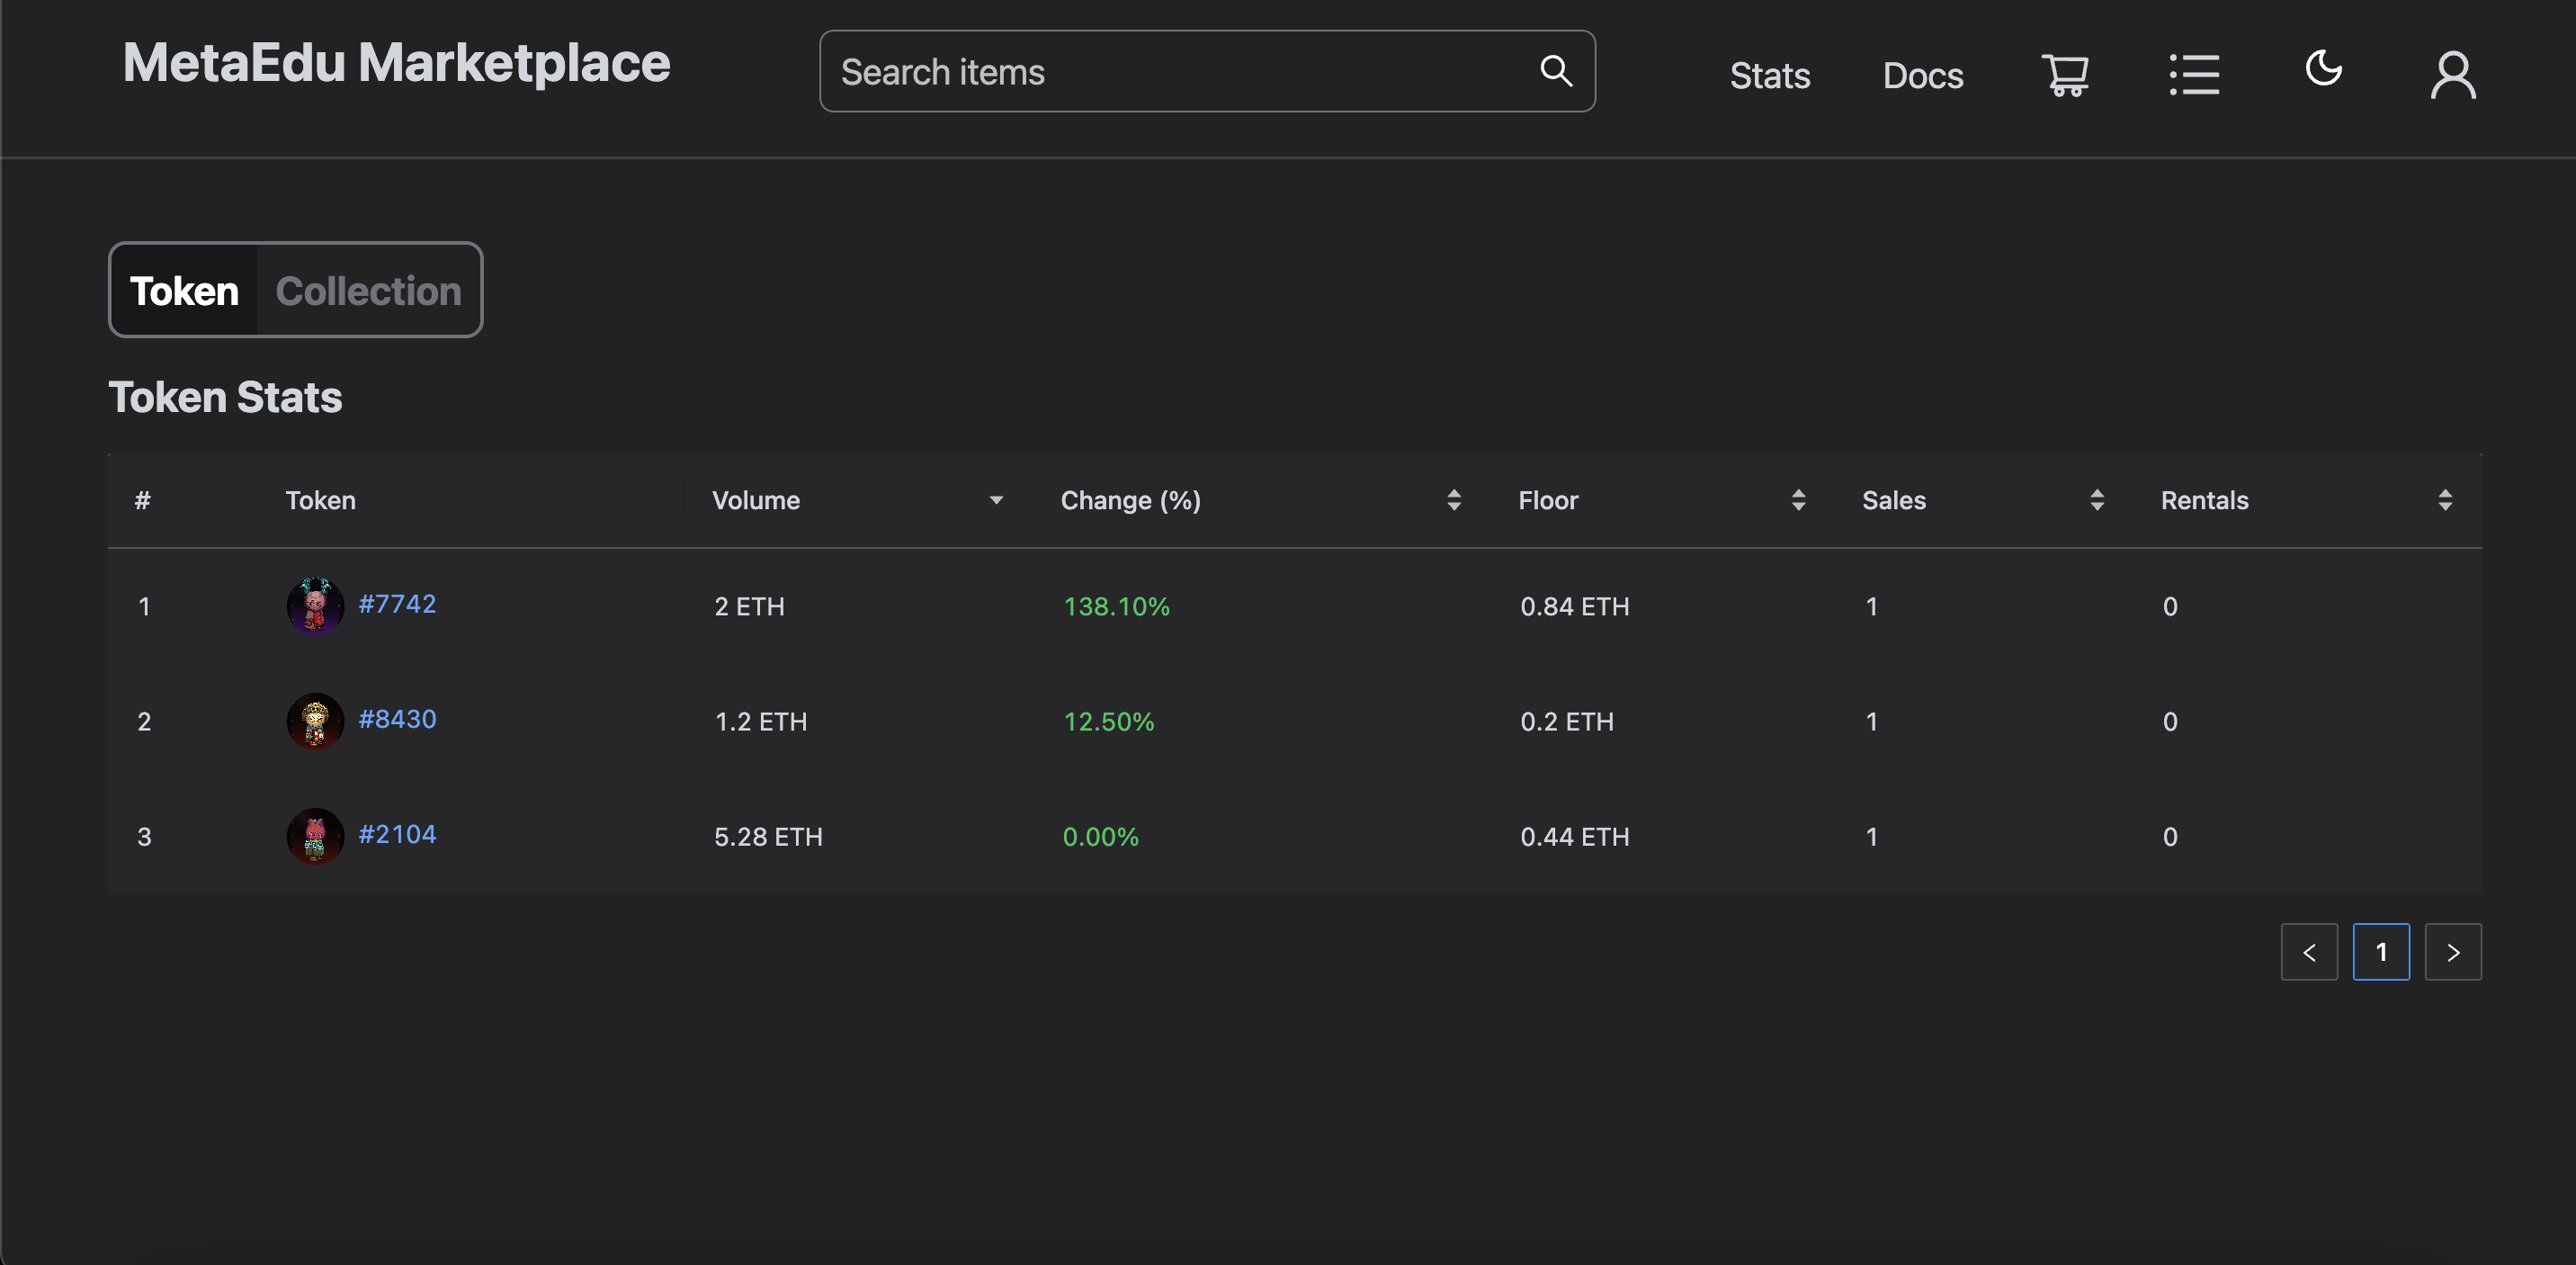
\includegraphics[scale=0.3]{gambar/img-frontend-stats.png}
  \caption{Halaman statistik}
  \label{fig:TokenStats}
\end{figure}

Halaman statistik berisi daftar token dan koleksi yang diurutkan berdasarkan parameter seperti \emph{Volume}, perubahan harga, \emph{floor} / harga terbawah, jumlah penjualan dan jumlah penyewaan.

\subsection{Halaman Dokumentasi}
\begin{figure} [H] \centering
  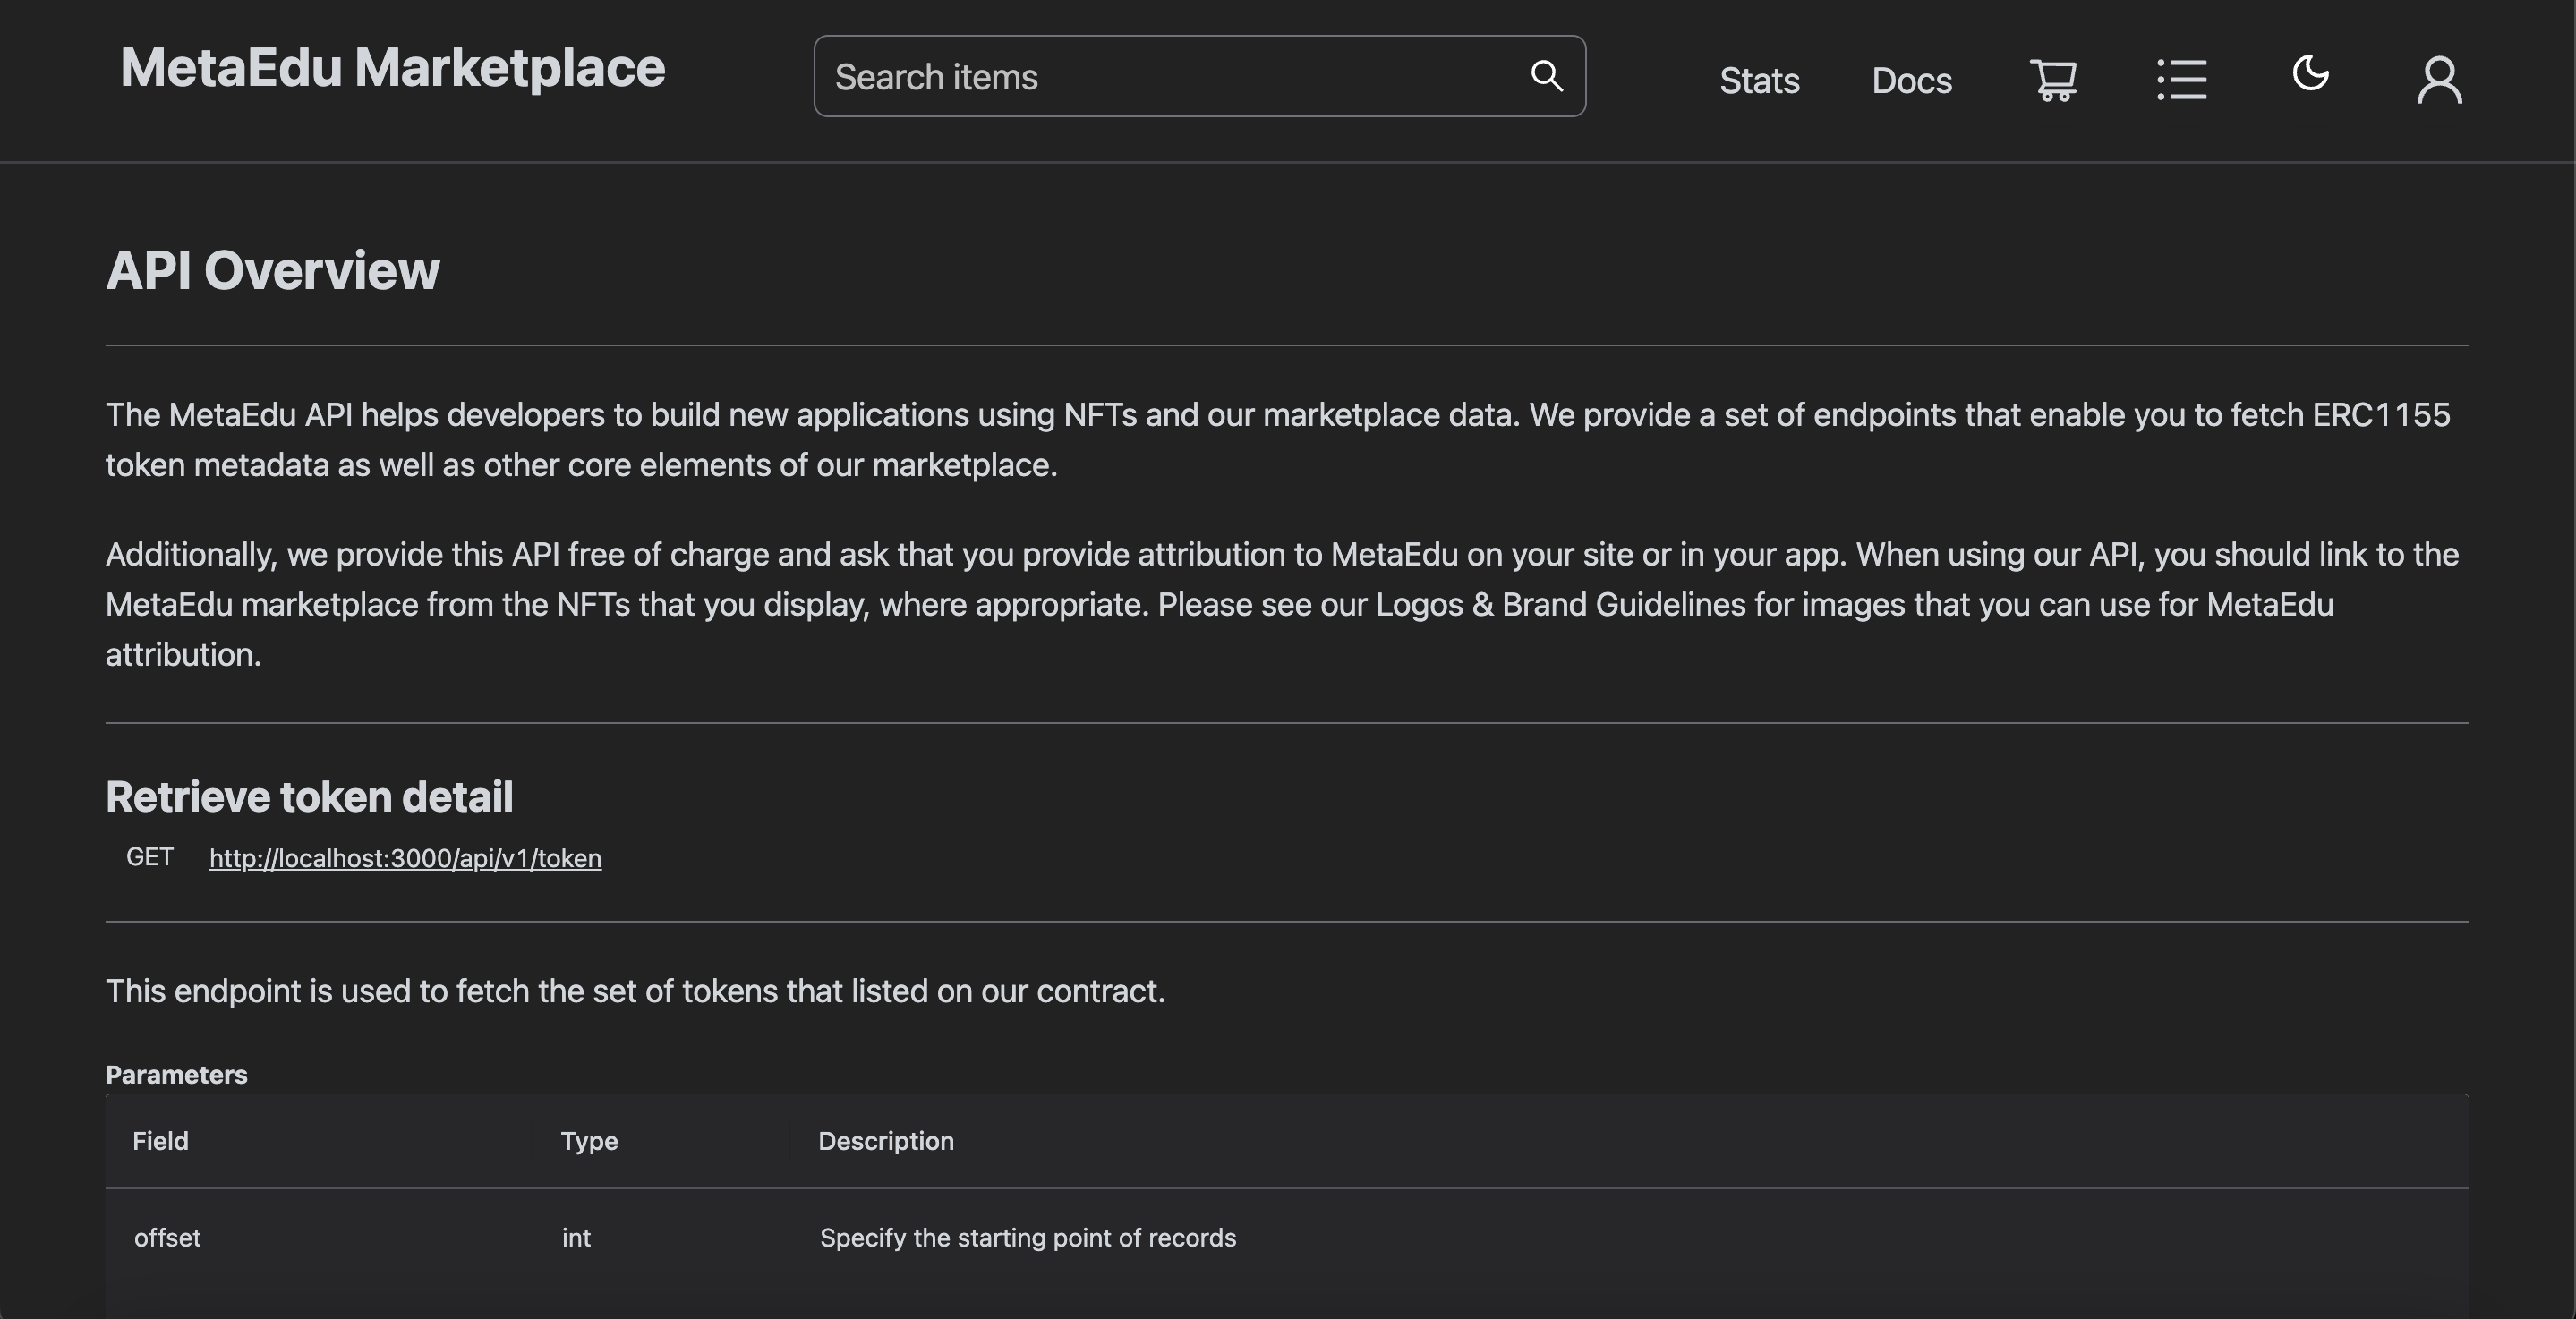
\includegraphics[scale=0.3]{gambar/img-frontend-api.png}
  \caption{Halaman dokumentasi}
  \label{fig:Docs}
\end{figure}

Halaman dokumentasi berisi informasi mengenai \emph{API} yang disedikan untuk \emph{platform} lain dapat memanfaatkan data dari \emph{NFT Marketplace} ini seperti data token, kepemilikan, dan penyewaan.

\section{Pengembangan \emph{Metaverse}} 

\emph{Metaverse} yang dikembangkan digunakan untuk menguji apakah API yang telah dikembangkan dapat diintegrasikan ke dalam \emph{metaverse} tersebut. Software yang digunakan untuk mengembangkan \emph{metaverse} ini adalah Unity. Untuk melakukan proses autentikasi mengunakan \emph{metamask} digunakan \emph{library} \emph{Web3Unity}. 

\subsection{Halaman Autentikas} 

\begin{figure} [H] \centering
  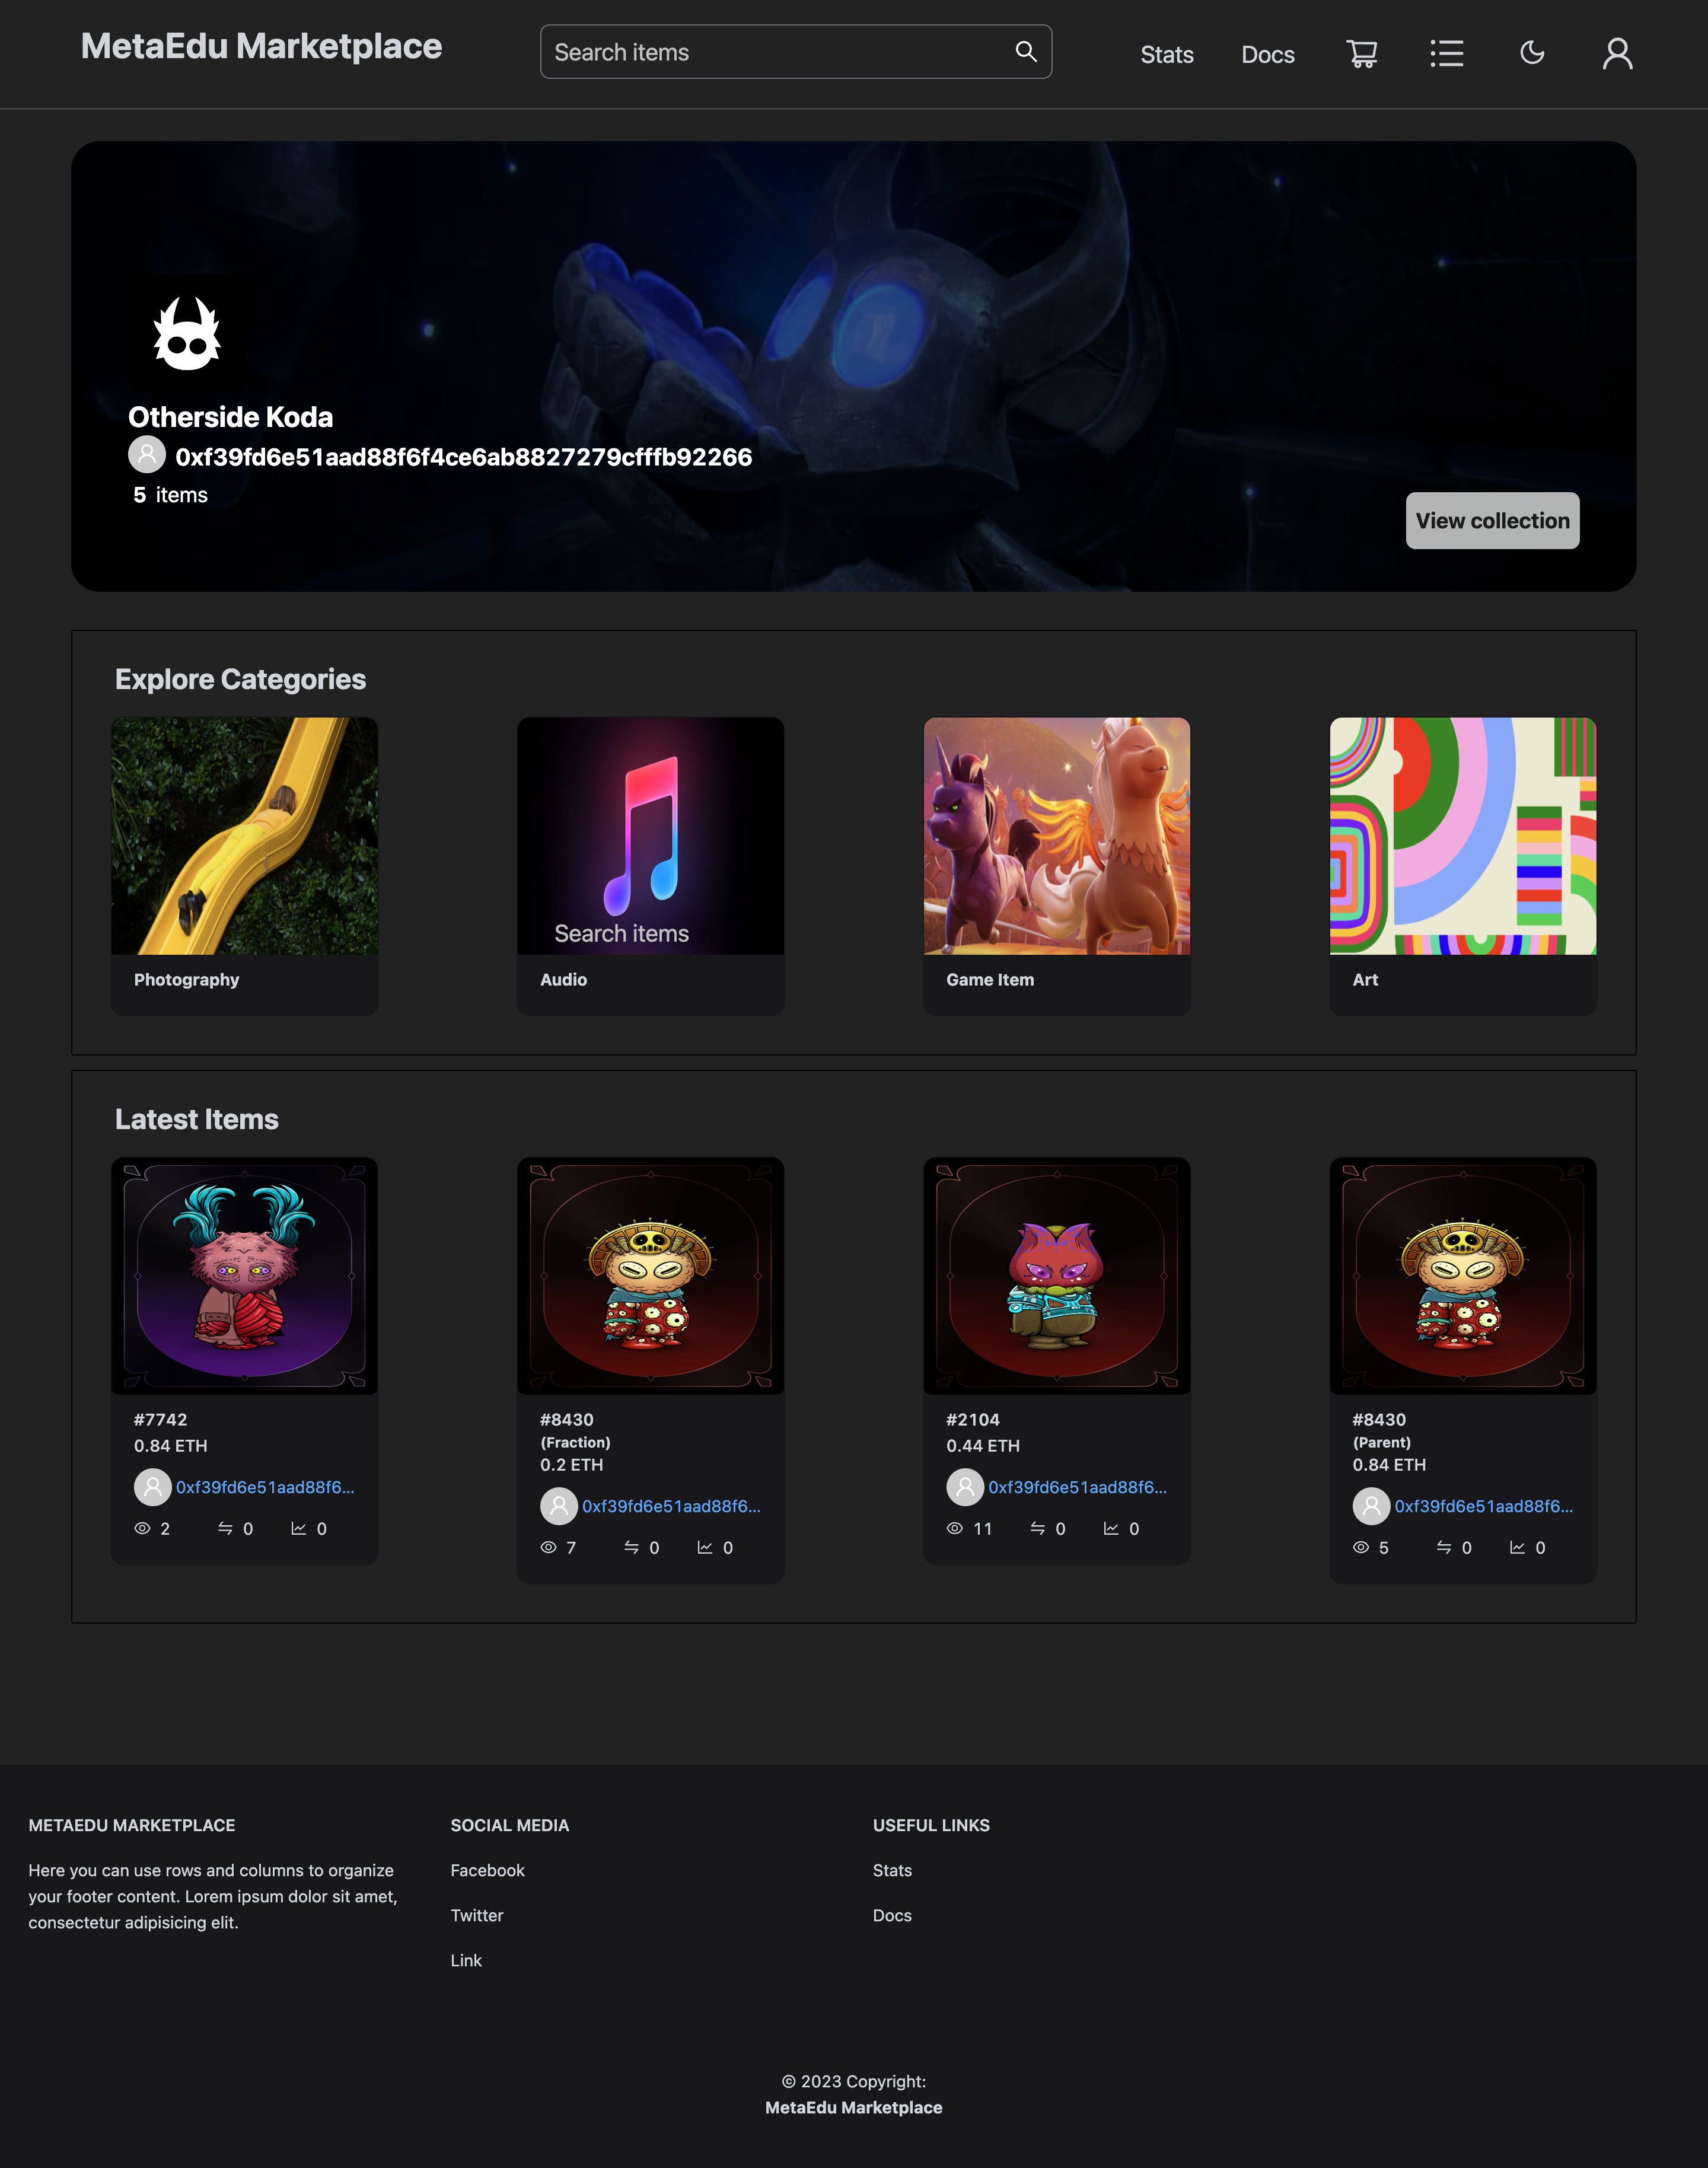
\includegraphics[scale=0.12]{gambar/img-frontend-index.png}
  \caption{Halaman awal \emph{NFT Marketplace}}
  \label{fig:NFTMarketplace}
\end{figure}

Tampilan awal \emph{NFT Marketplace}, menampilkan koleksi \emph{token}, kategori \emph{token}, dan \emph{token} terbaru.

\begin{figure} [H] \centering
  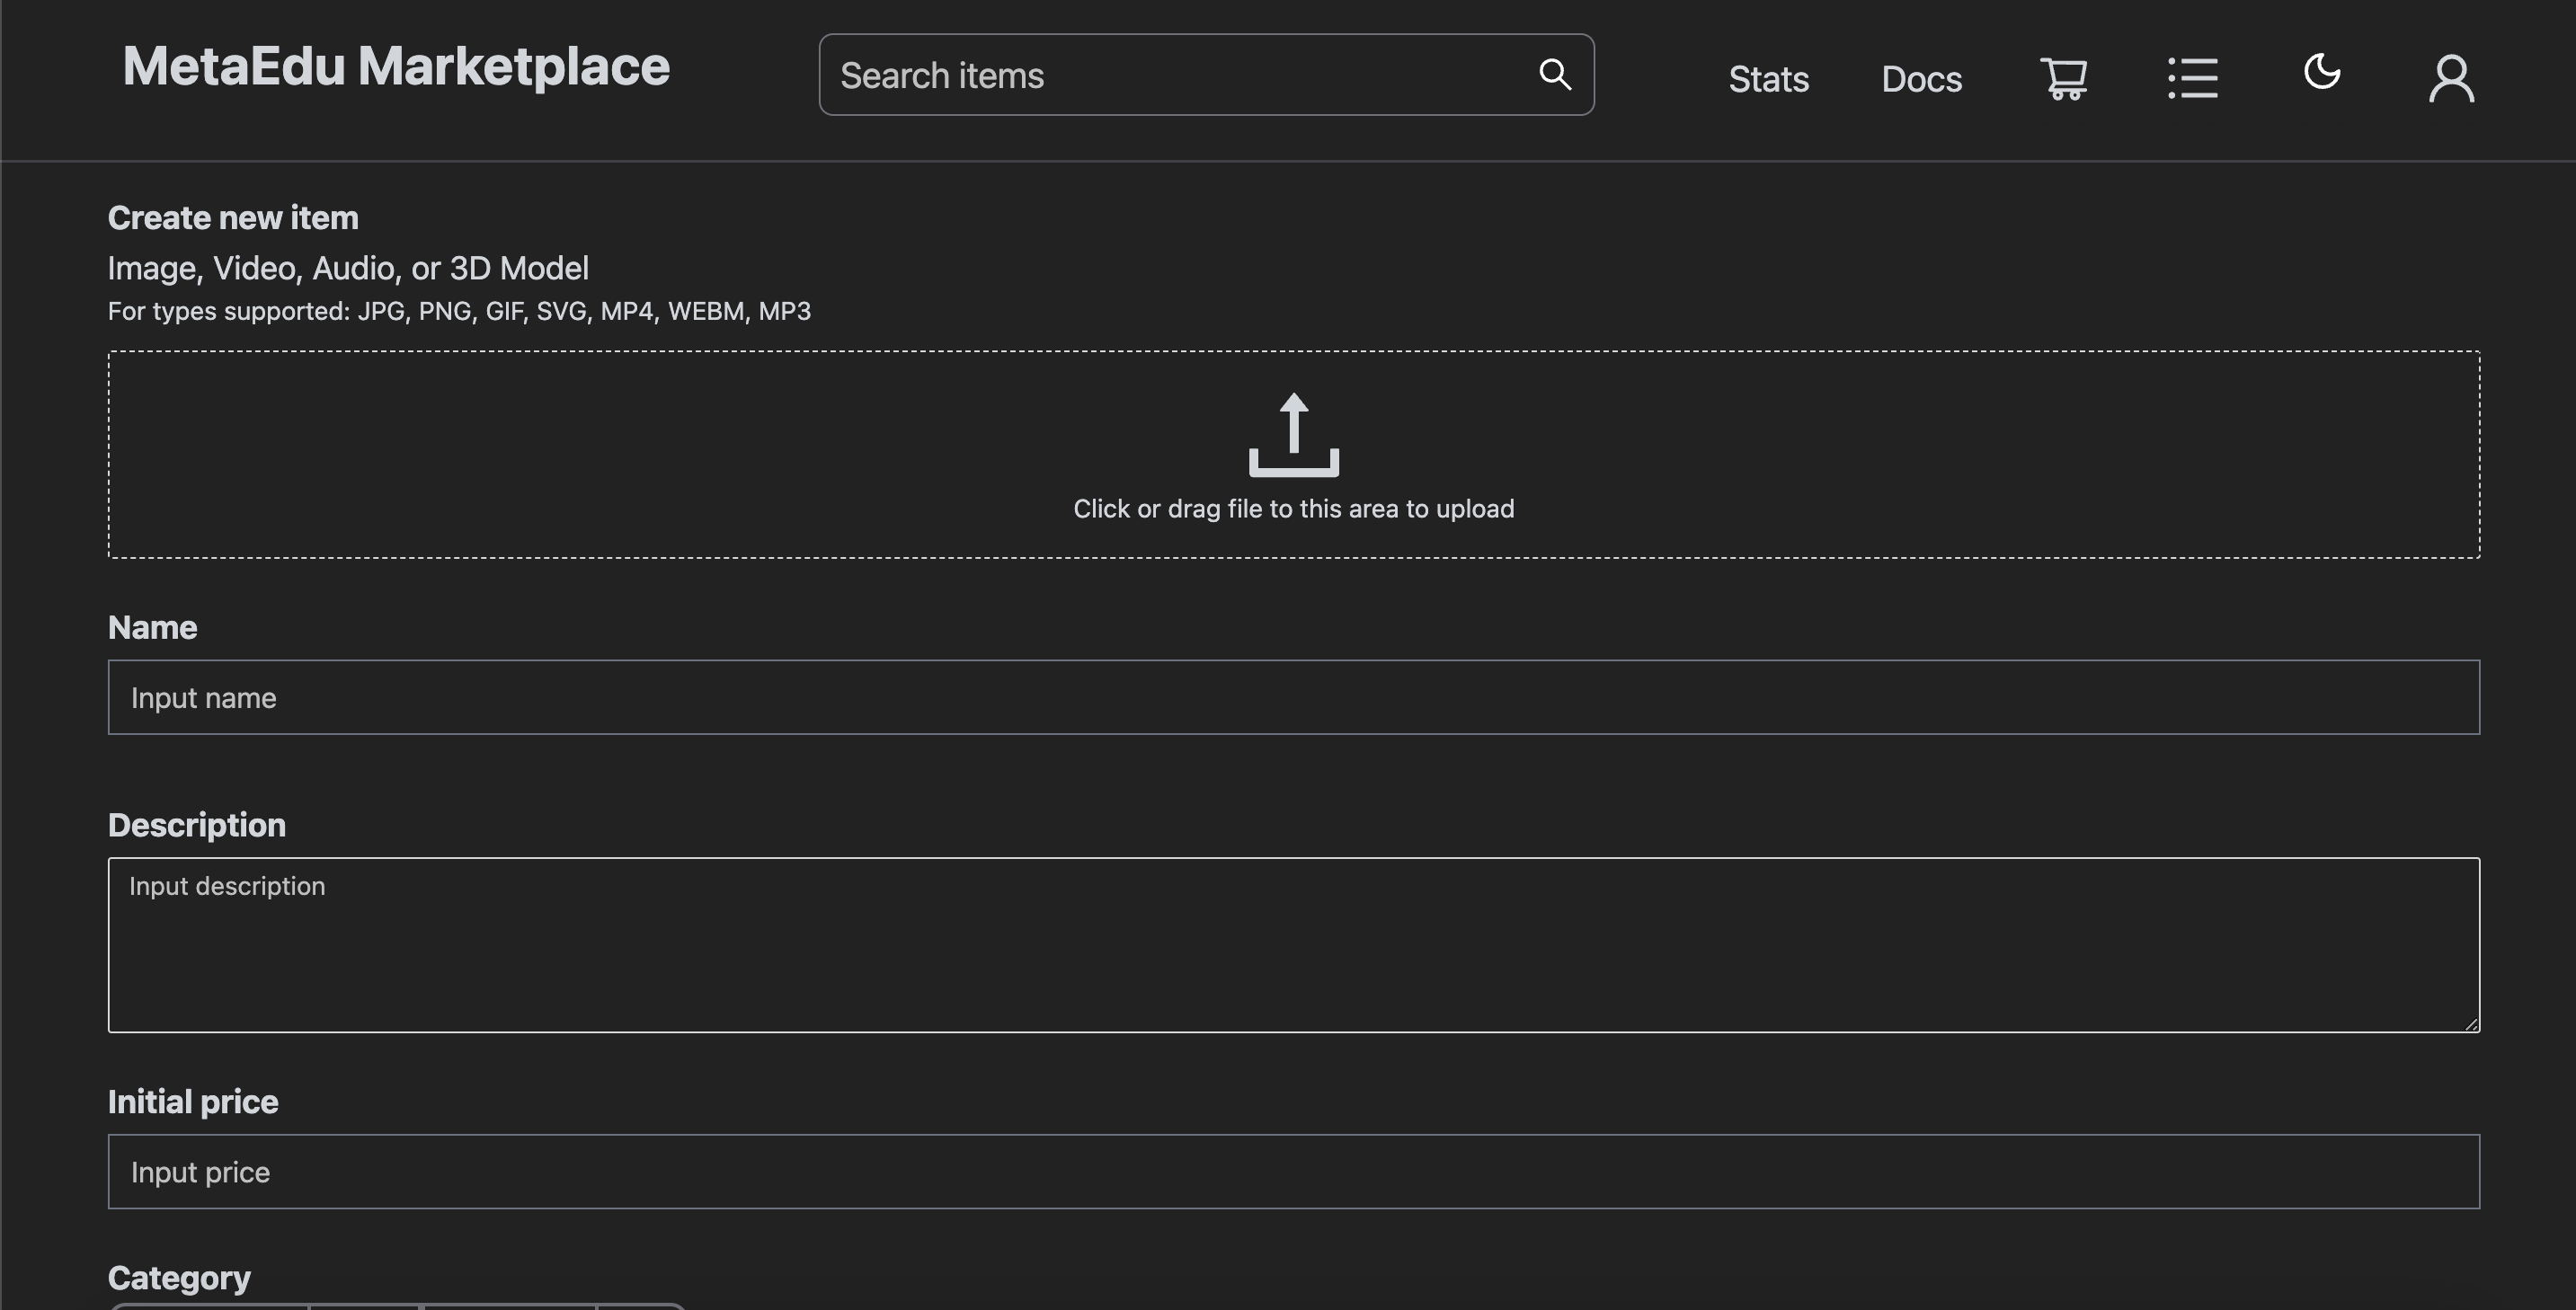
\includegraphics[scale=0.3]{gambar/img-frontend-add-token.png}
  \caption{Halaman \emph{Minting Token}}
  \label{fig:TokenMinting}
\end{figure}

Halaman \emph{Minting token} merupakan halaman yang digunakan \emph{user} untuk membuat \emph{token} baru. Untuk membuat \emph{token} baru, \emph{user} perlu memasukan \emph{image} \emph{token}, nama \emph{token}, harga awal, suplai, dan koleksi. 

\subsection{Halaman Detail \emph{Token}}

\begin{figure} [H] \centering
  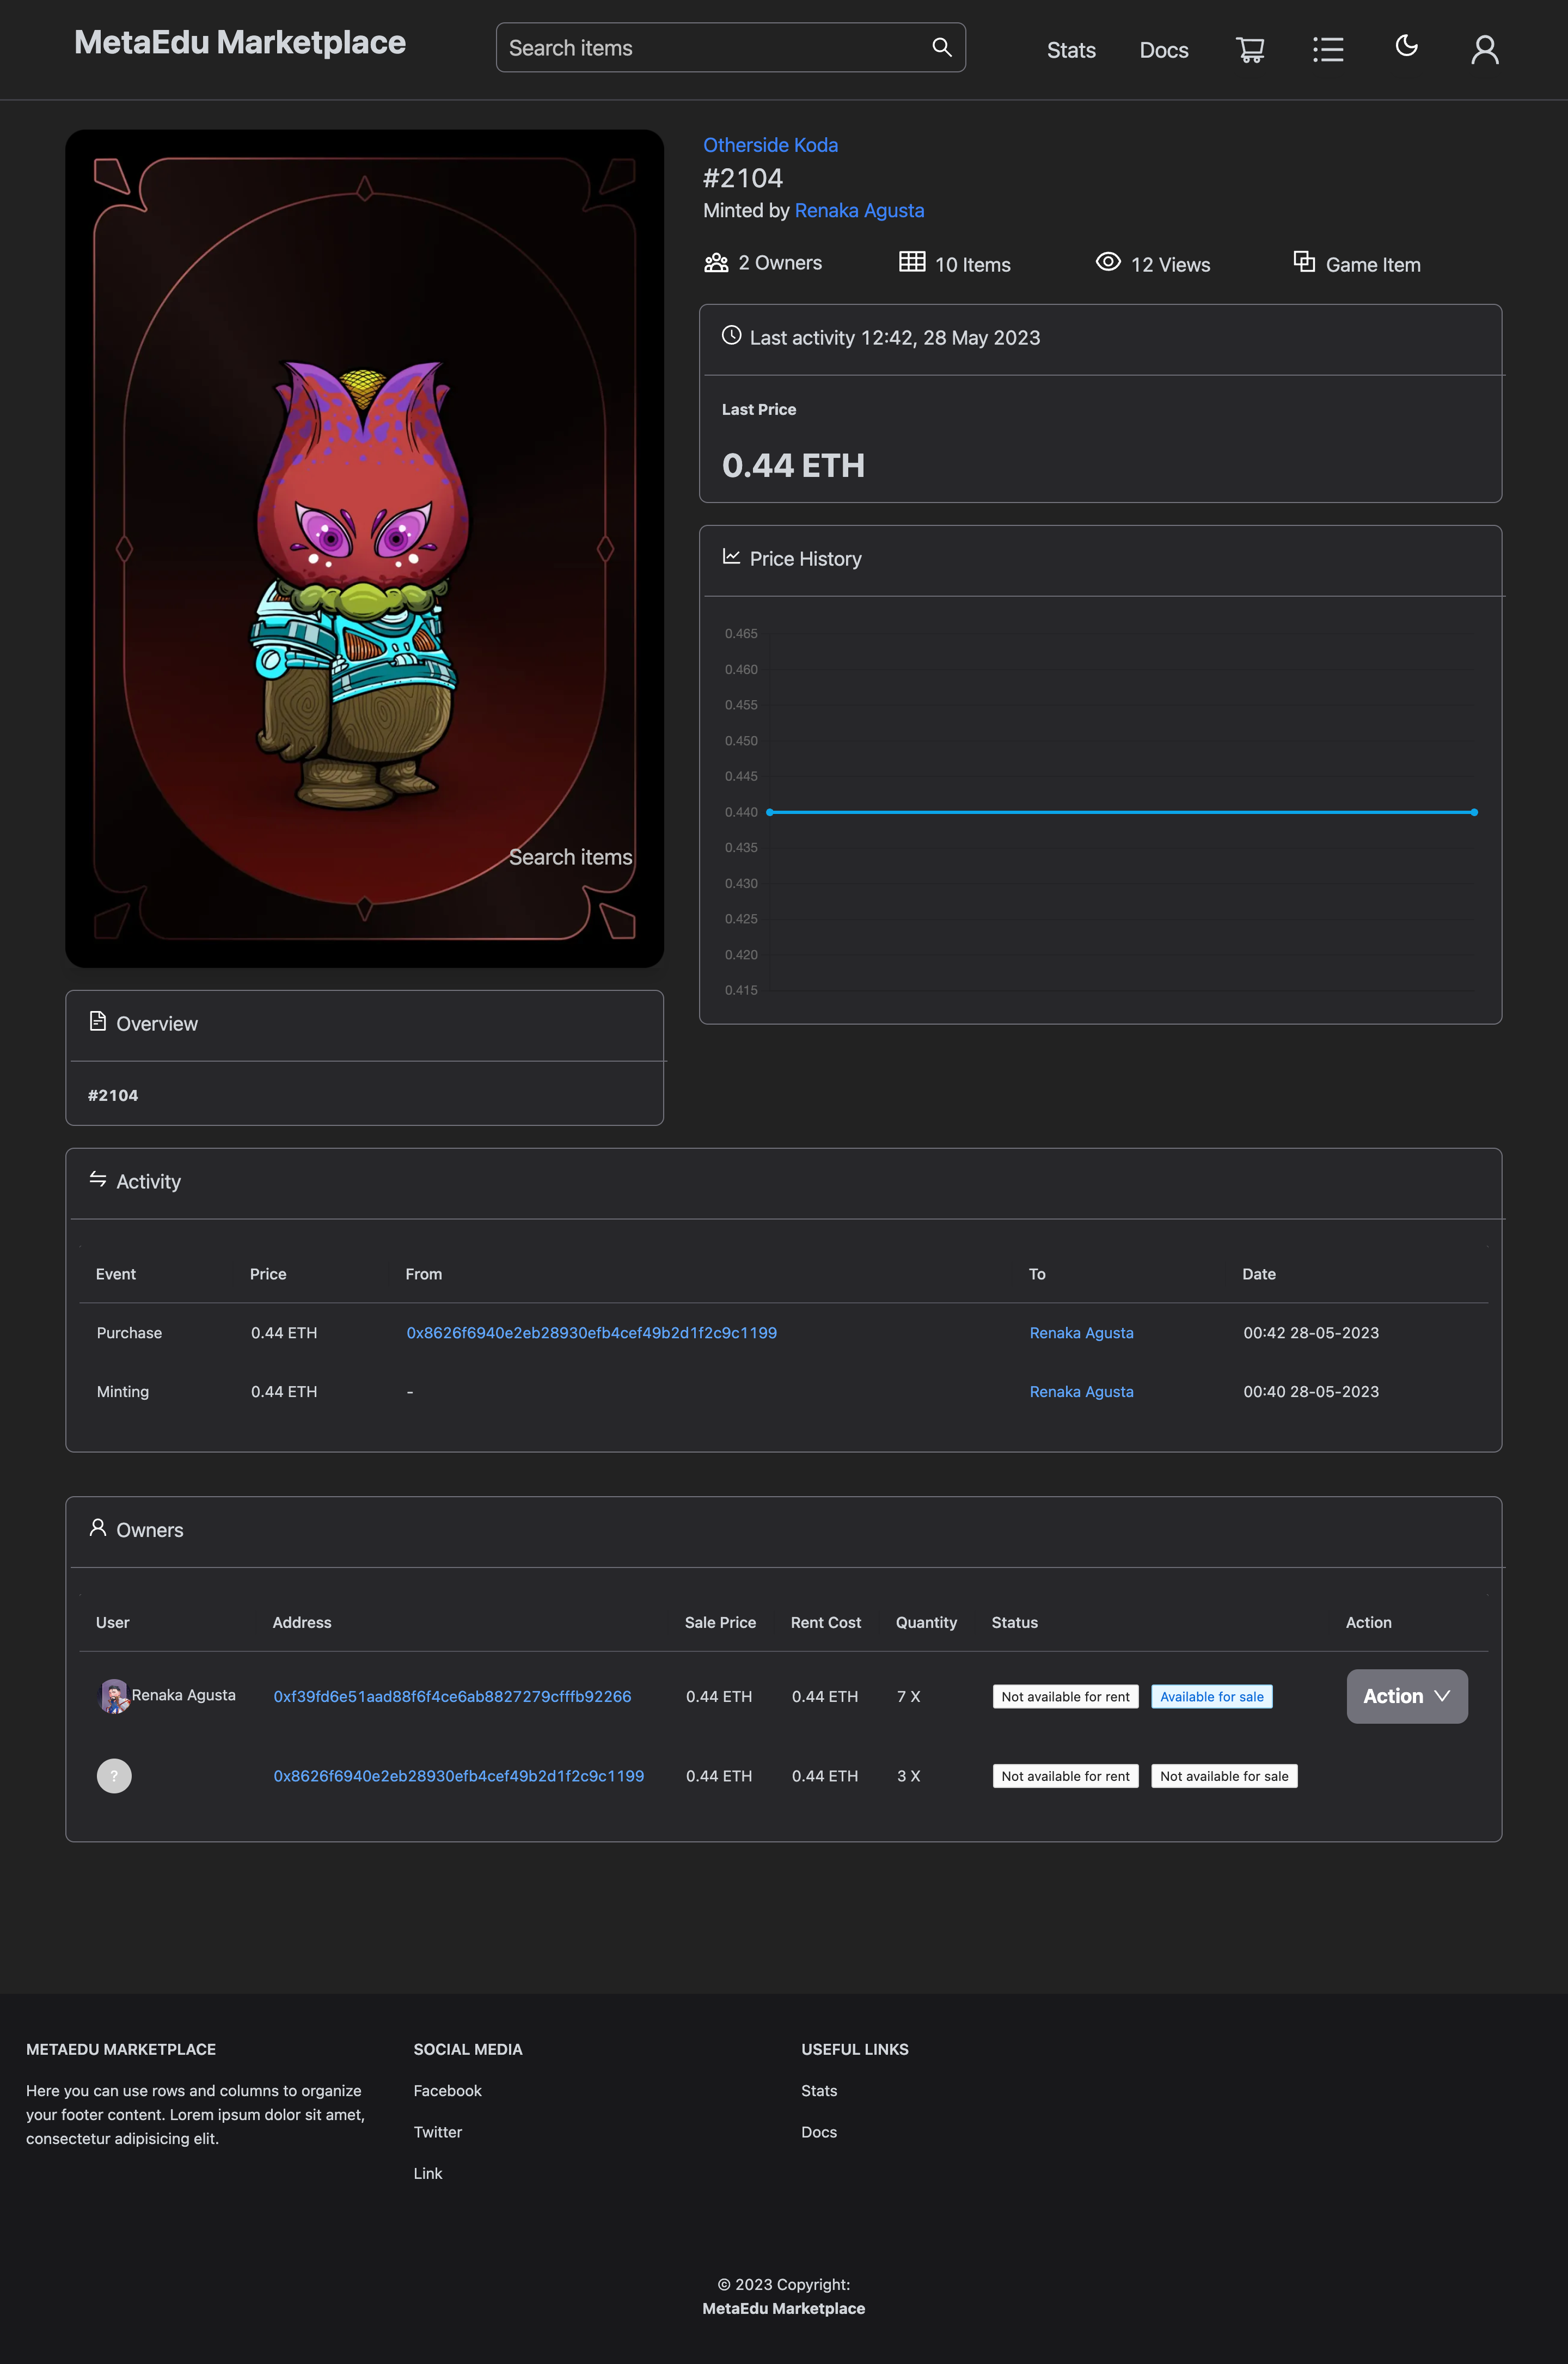
\includegraphics[scale=0.1]{gambar/img-frontend-token-detail.png}
  \caption{Halaman detail \emph{Token}}
  \label{fig:TokenDetail}
\end{figure}

Halaman detail \emph{token} menampilkan informasi-informasi mengenai nama \emph{token}, harga terakhir, pergerakan harga, riwayat transaksi, daftar kepemilkan dan lainnya. 

\subsection{Halaman Pencarian \emph{Token}}
\begin{figure} [H] \centering
  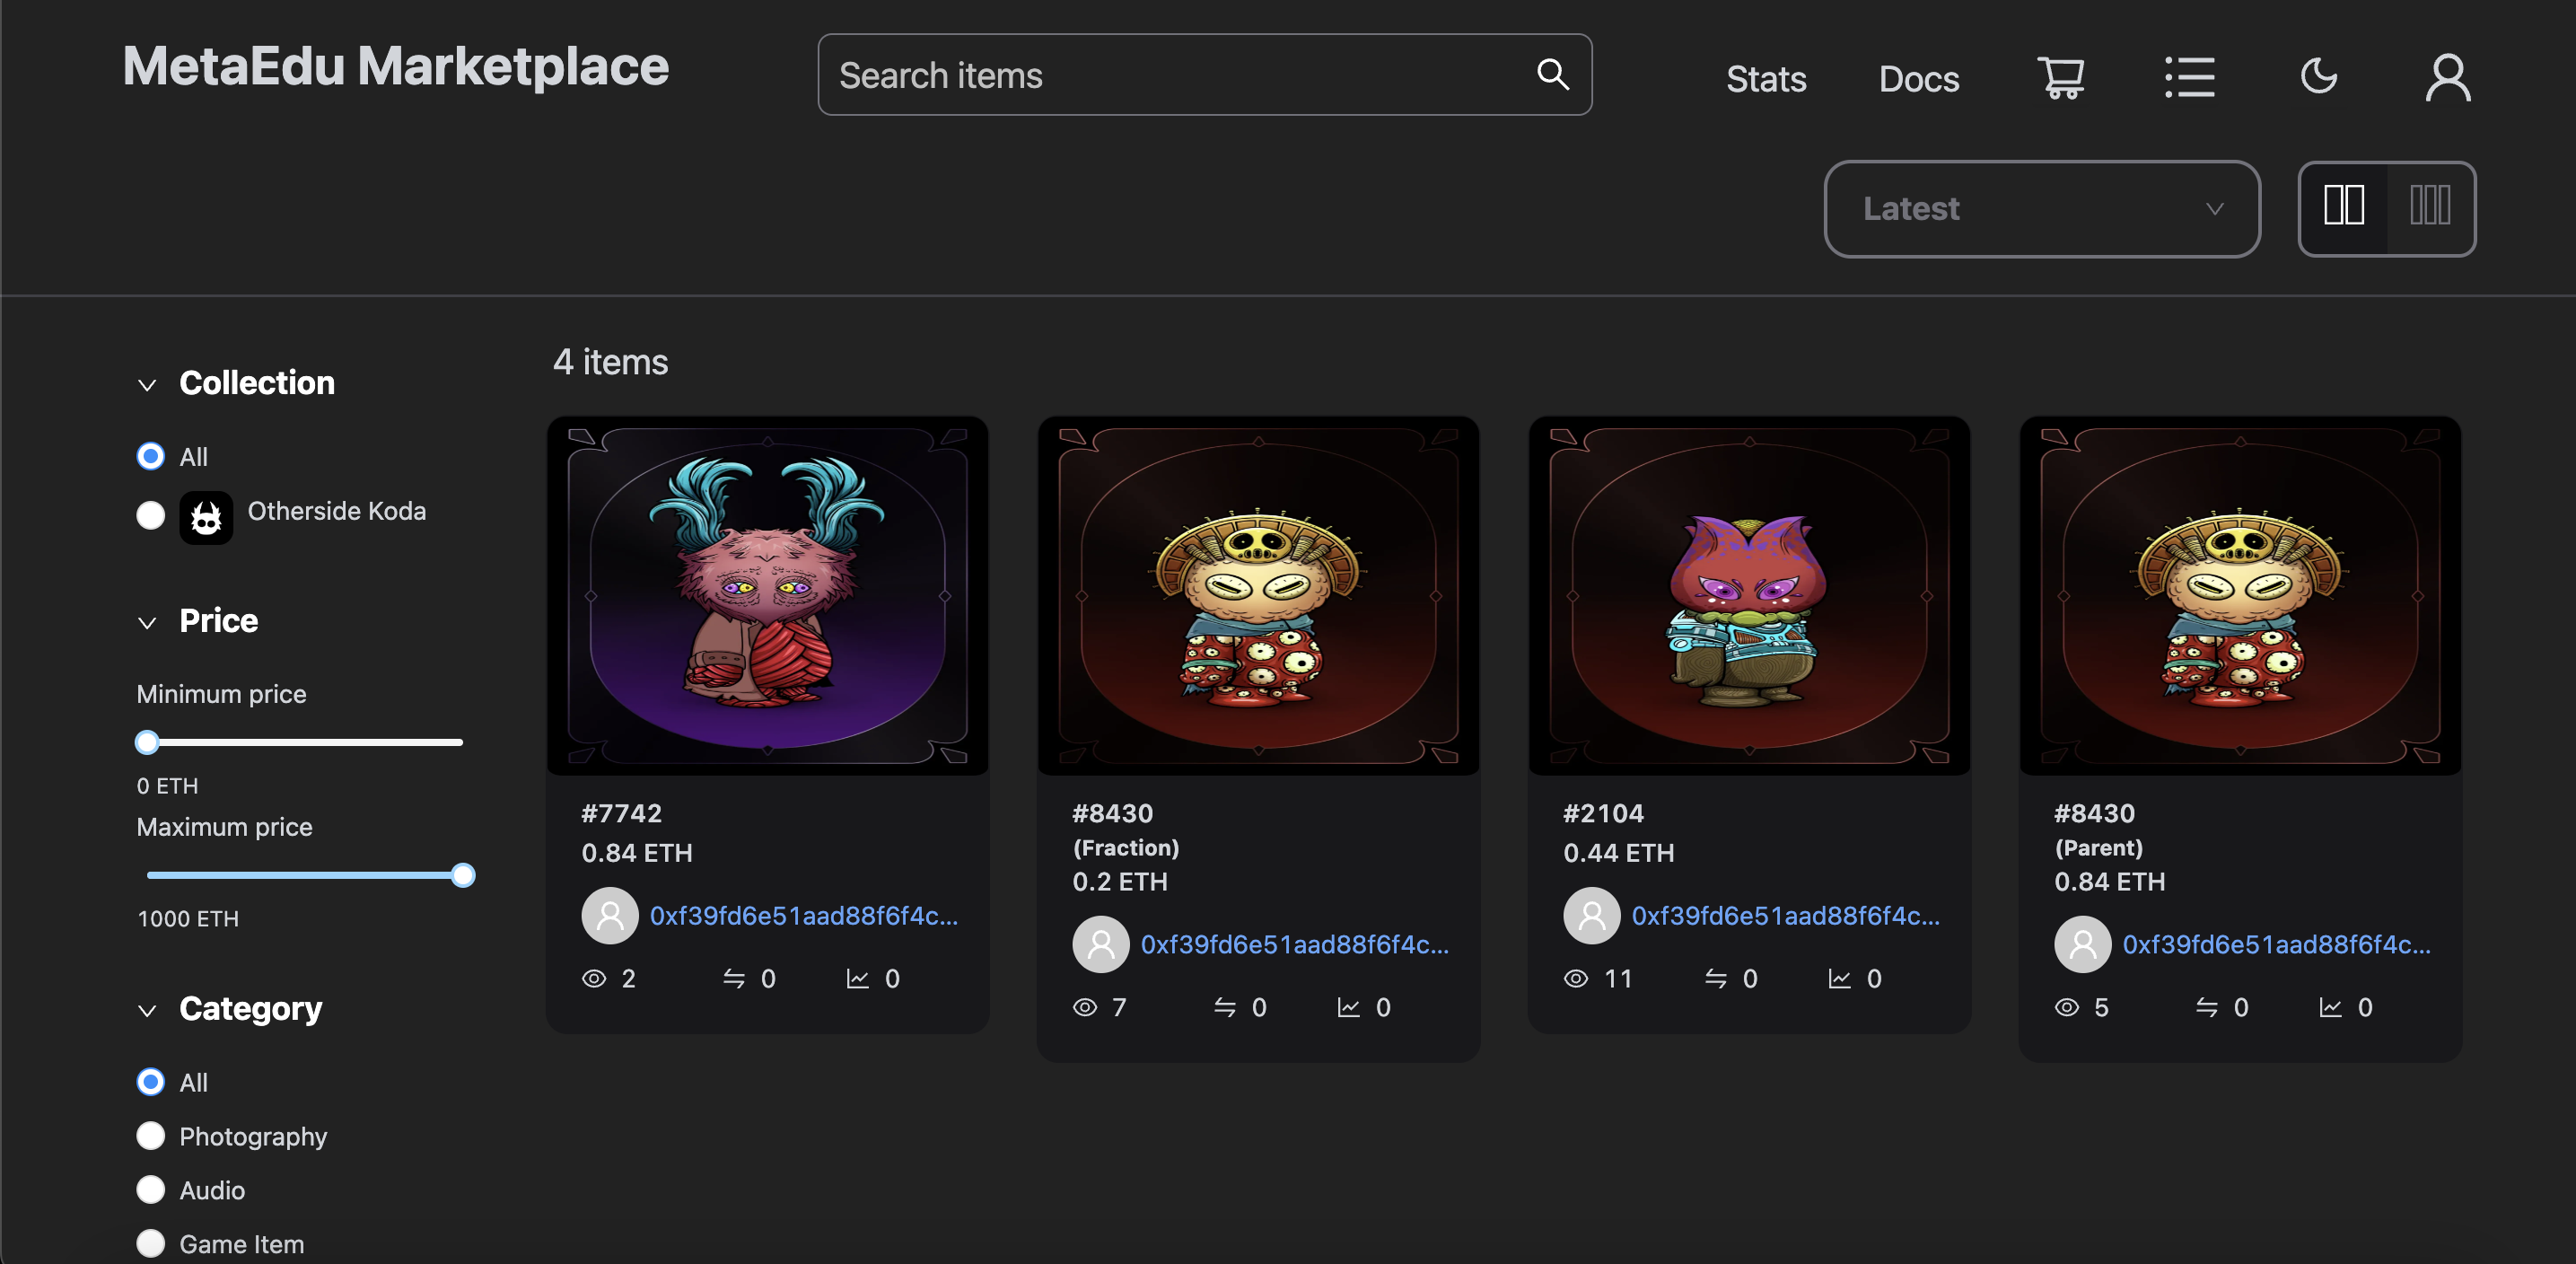
\includegraphics[scale=0.3]{gambar/img-frontend-search.png}
  \caption{Halaman pencarian \emph{Token}}
  \label{fig:TokenSearch}
\end{figure}

Halaman pencarian \emph{token} digunakan oleh \emph{user} untuk mencari \emph{token} tertentu berdasarkan nama, kategori, harga, dan koleksi.

\subsection{Halaman Detail Koleksi}
\begin{figure} [H] \centering
  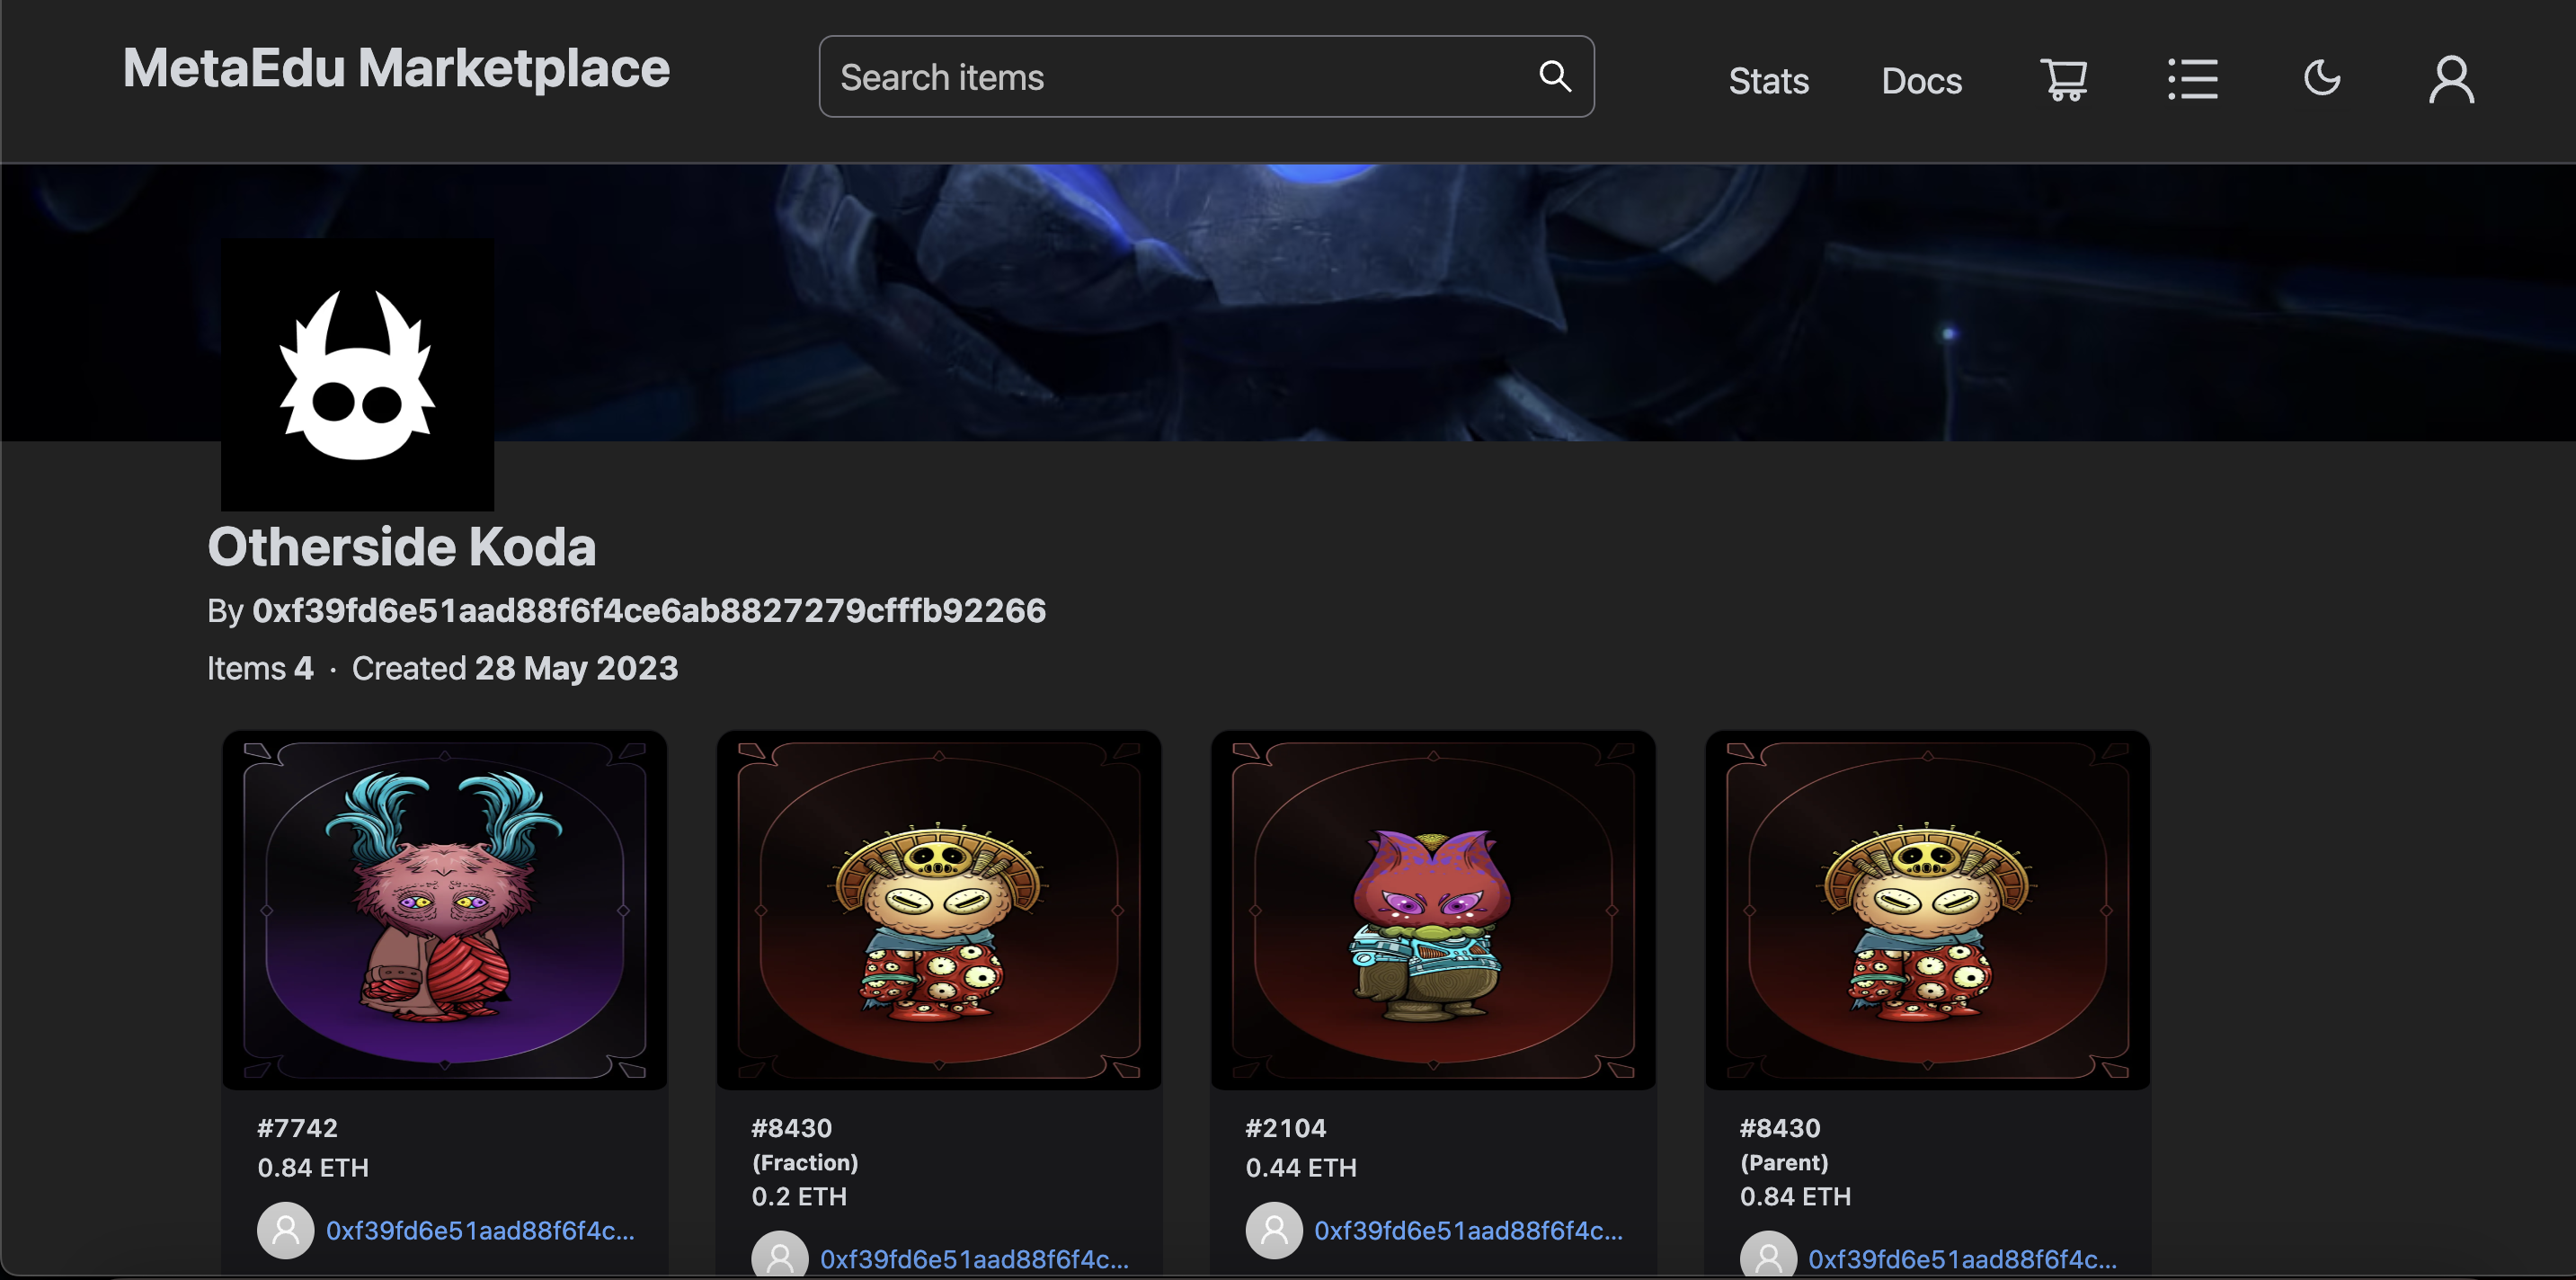
\includegraphics[scale=0.3]{gambar/img-frontend-collection.png}
  \caption{Halaman detail koleksi}
  \label{fig:CollectionDetail}
\end{figure}

Halaman detail koleksi berisi daftar token yang terkait dengan kolesi tersebut.

\subsection{Halaman Statistik}
\begin{figure} [H] \centering
  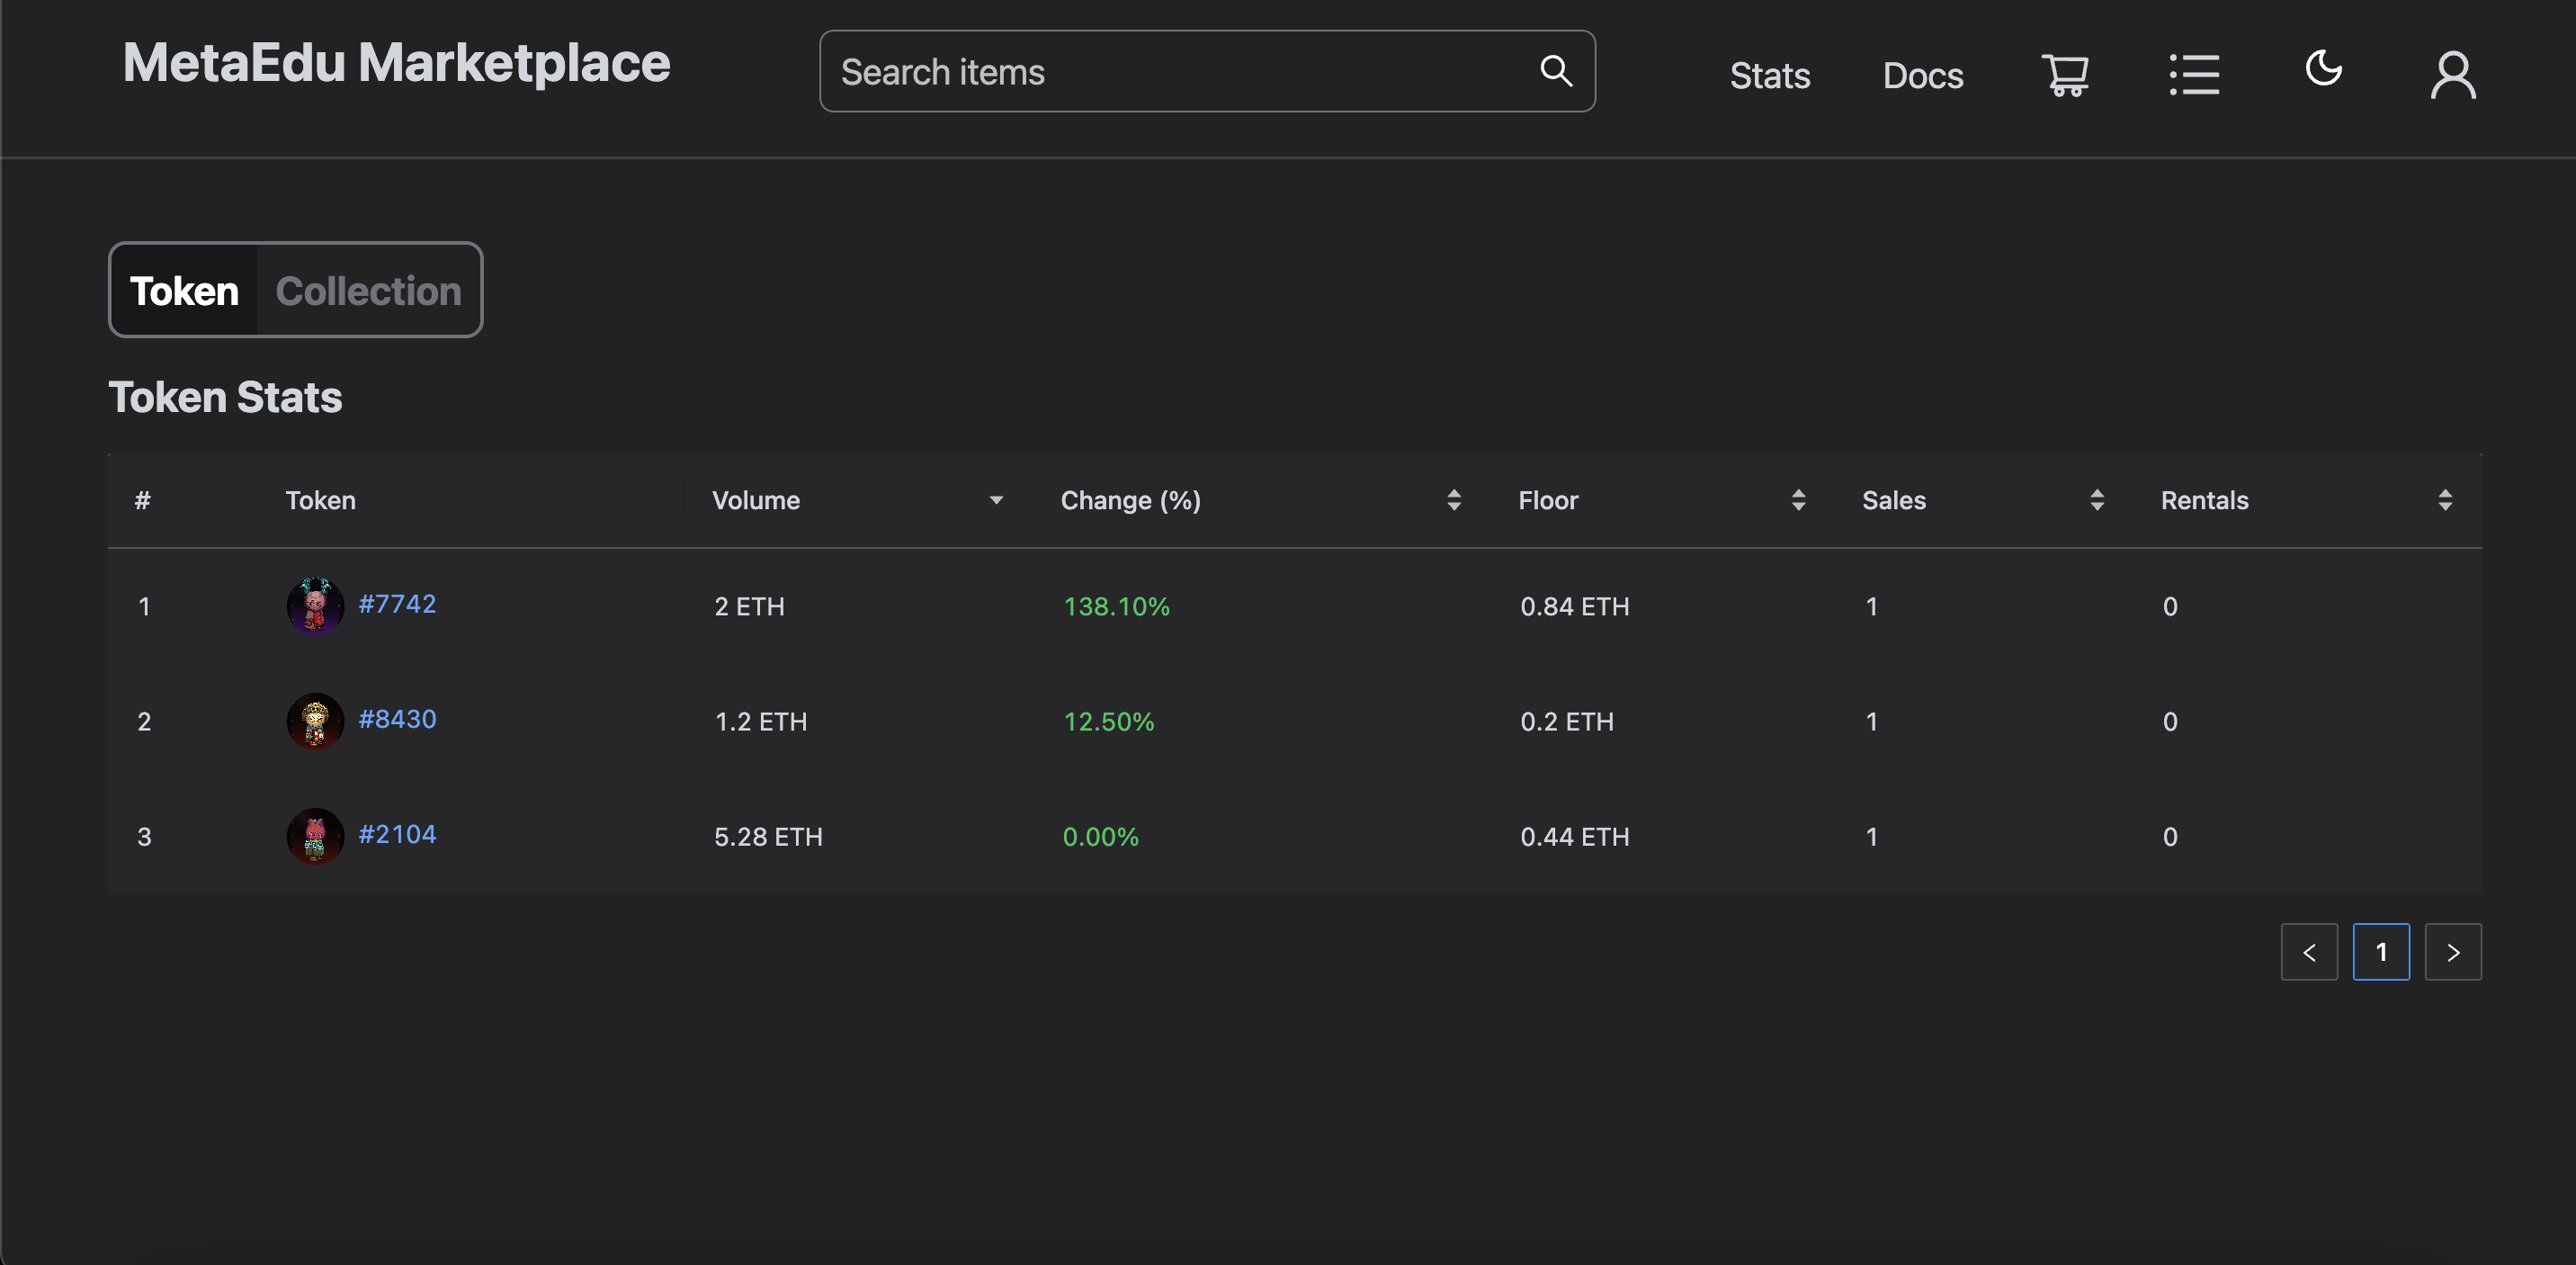
\includegraphics[scale=0.3]{gambar/img-frontend-stats.png}
  \caption{Halaman statistik}
  \label{fig:TokenStats}
\end{figure}

Halaman statistik berisi daftar token dan koleksi yang diurutkan berdasarkan parameter seperti \emph{Volume}, perubahan harga, \emph{floor} / harga terbawah, jumlah penjualan dan jumlah penyewaan.

\subsection{Halaman Dokumentasi}
\begin{figure} [H] \centering
  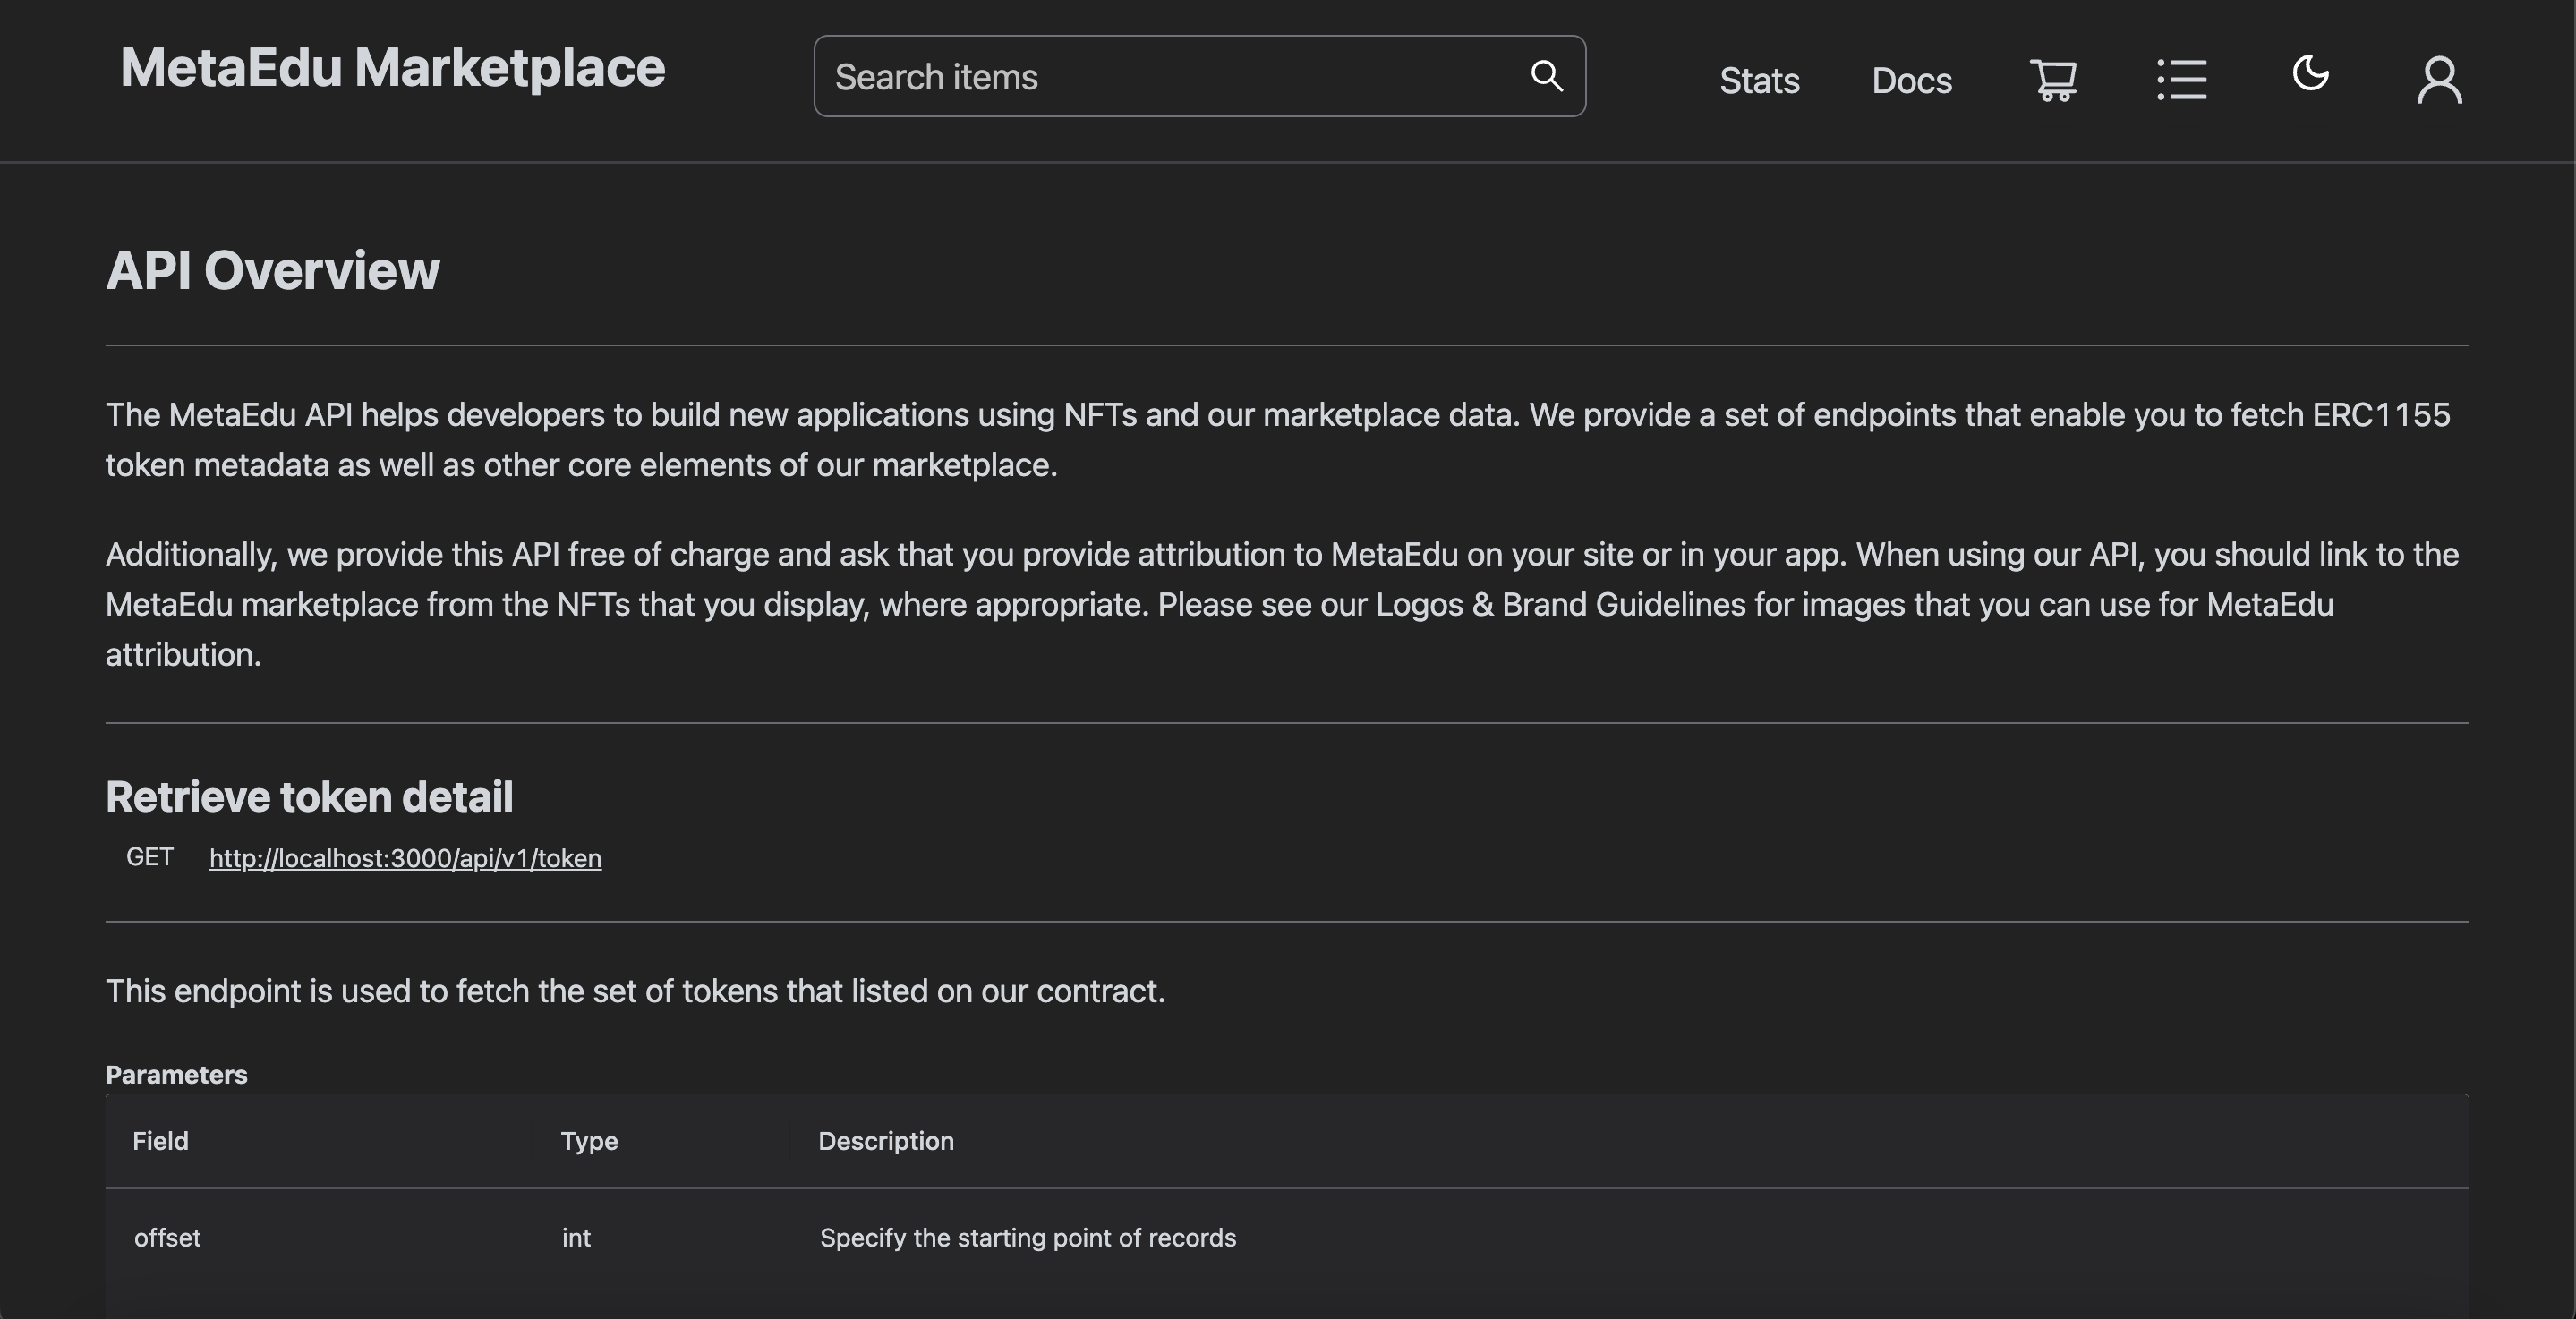
\includegraphics[scale=0.3]{gambar/img-frontend-api.png}
  \caption{Halaman dokumentasi}
  \label{fig:Docs}
\end{figure}

Halaman dokumentasi berisi informasi mengenai \emph{API} yang disedikan untuk \emph{platform} lain dapat memanfaatkan data dari \emph{NFT Marketplace} ini seperti data token, kepemilikan, dan penyewaan.

\subsection{API Marketplace} 

API Marketplace digunakan untuk memperoleh berbagai data dari \emph{database} yang pada \emph{web marketplace} maupun \emph{metaverse}.

\begin{figure} [H] \centering
  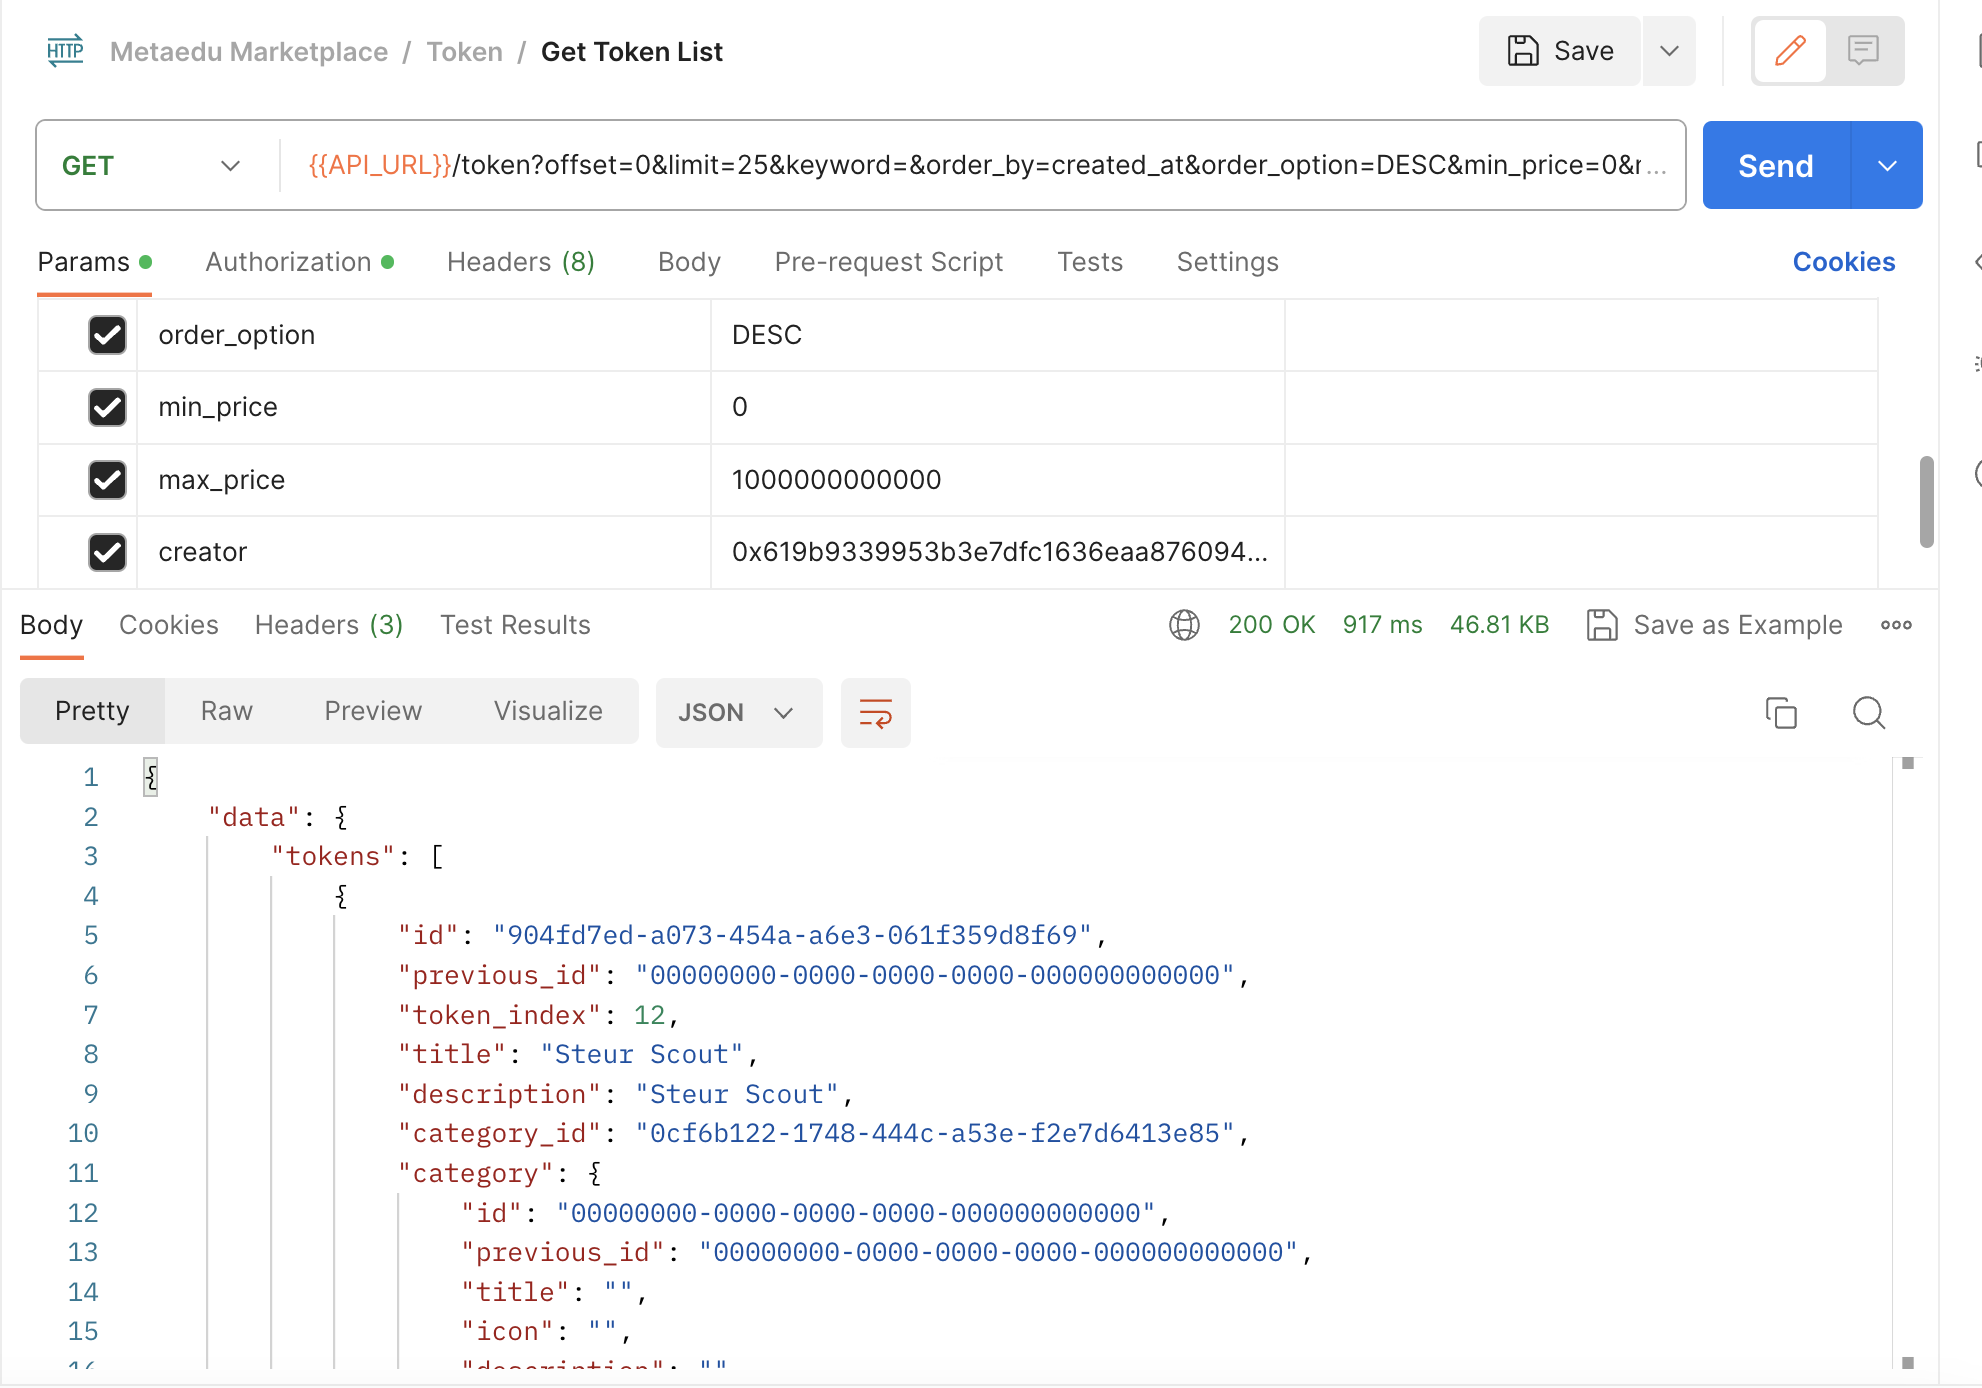
\includegraphics[scale=0.3]{gambar/img-api-tokens.png}
  \caption{\emph{API token} }
  \label{fig:APITokens}
\end{figure}

\emph{API} token memiliki \emph{prefix \textbf{\textbackslash token}} dan digunakan memperoleh seluruh data token yang disimpan dalam \emph{table tokens}. 

\begin{figure} [H] \centering
  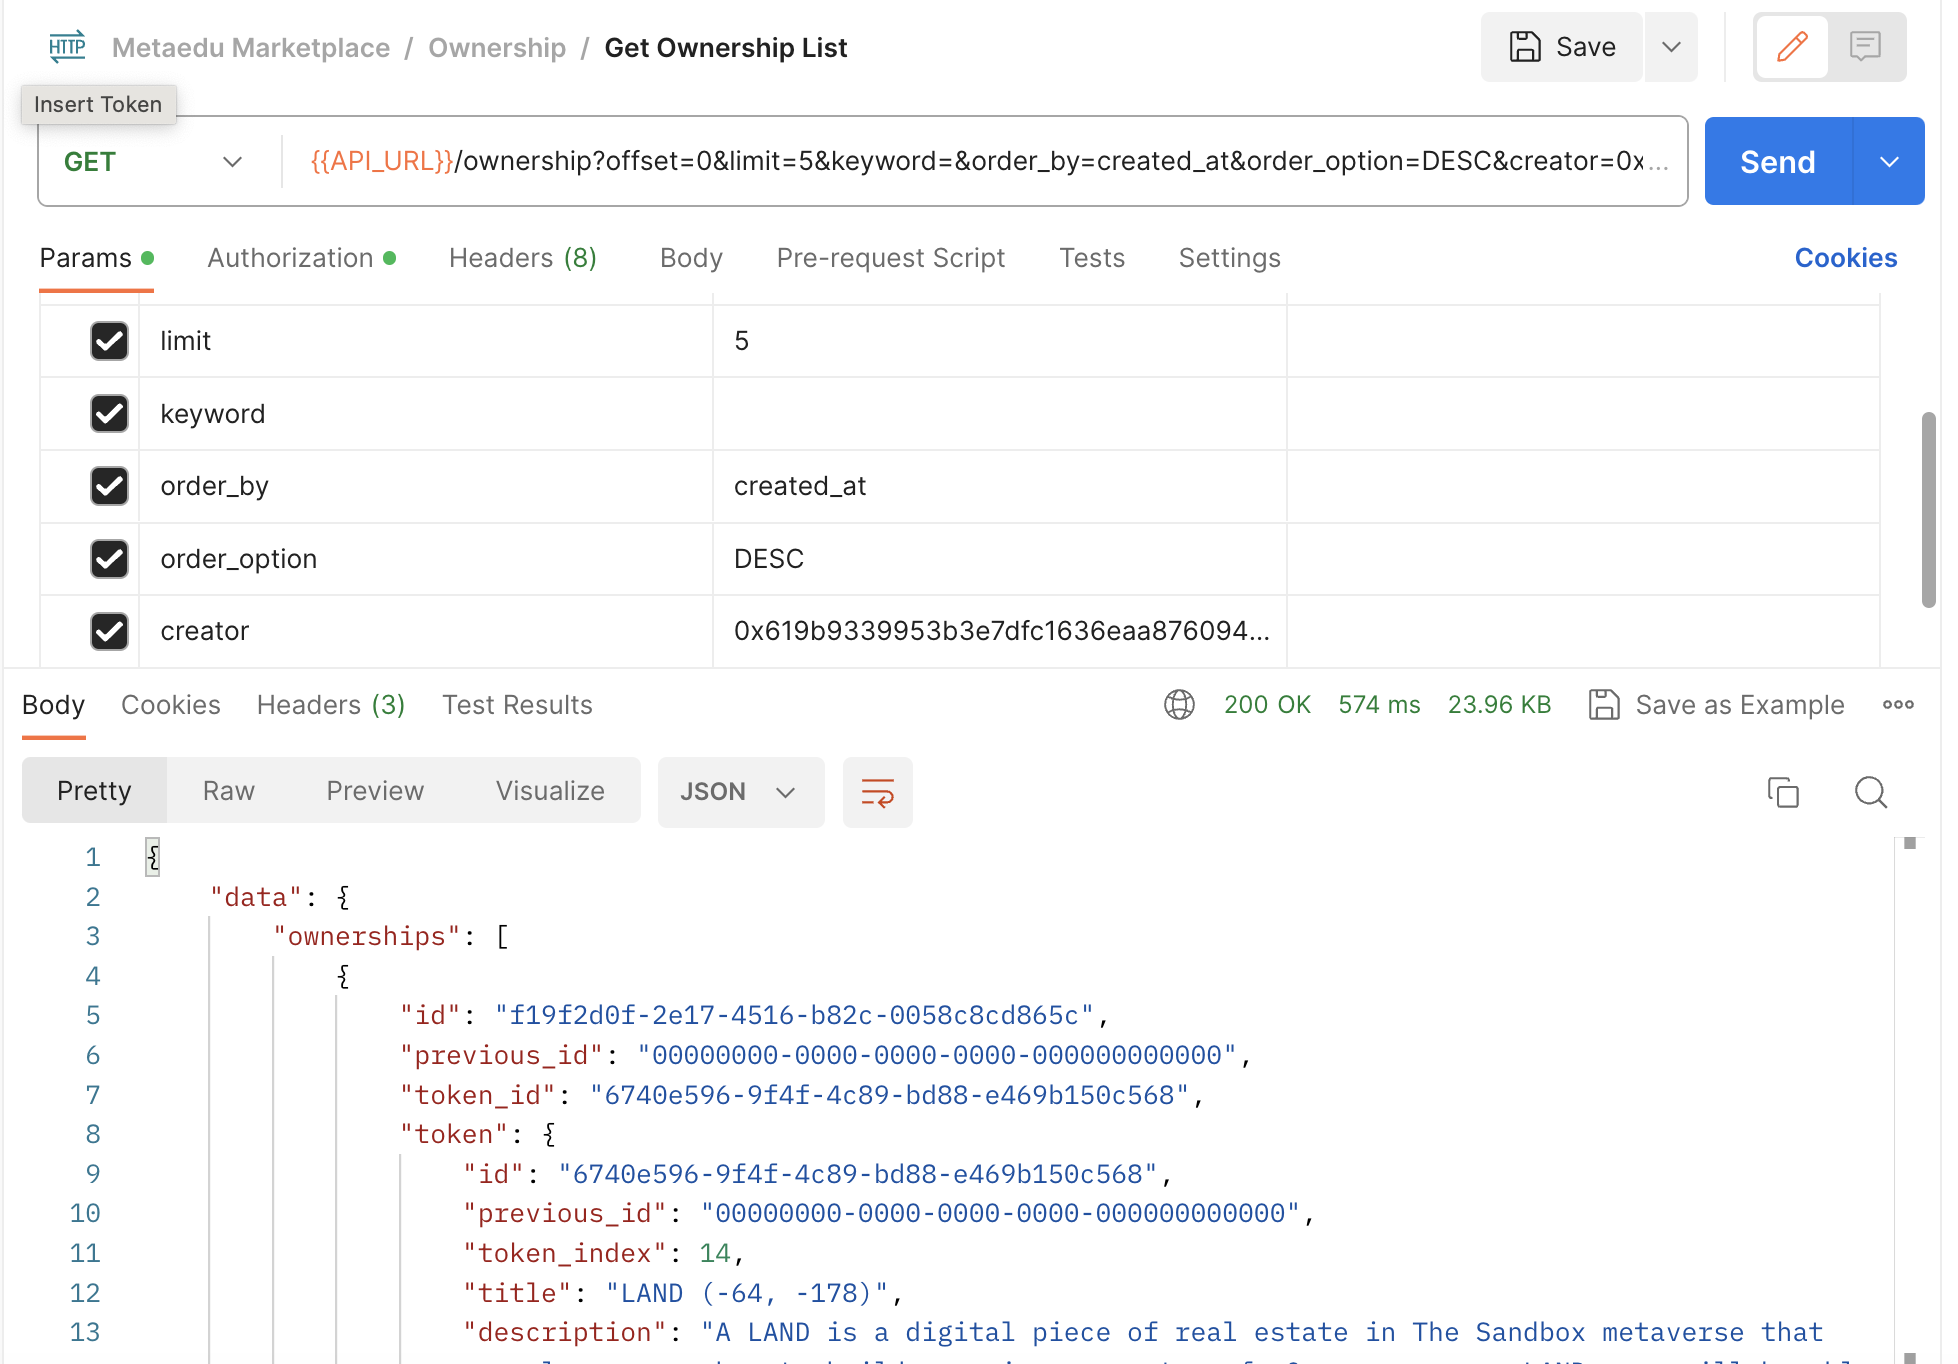
\includegraphics[scale=0.3]{gambar/img-api-ownerships.png}
  \caption{\emph{API token} }
  \label{fig:APIOwnerships}
\end{figure}

\emph{API} ownerships memiliki \emph{prefix \textbf{\textbackslash ownership}} dan digunakan memperoleh seluruh data kepemilikan token oleh pengguna yang disimpan dalam \emph{table ownerships}. 

\begin{figure} [H] \centering
  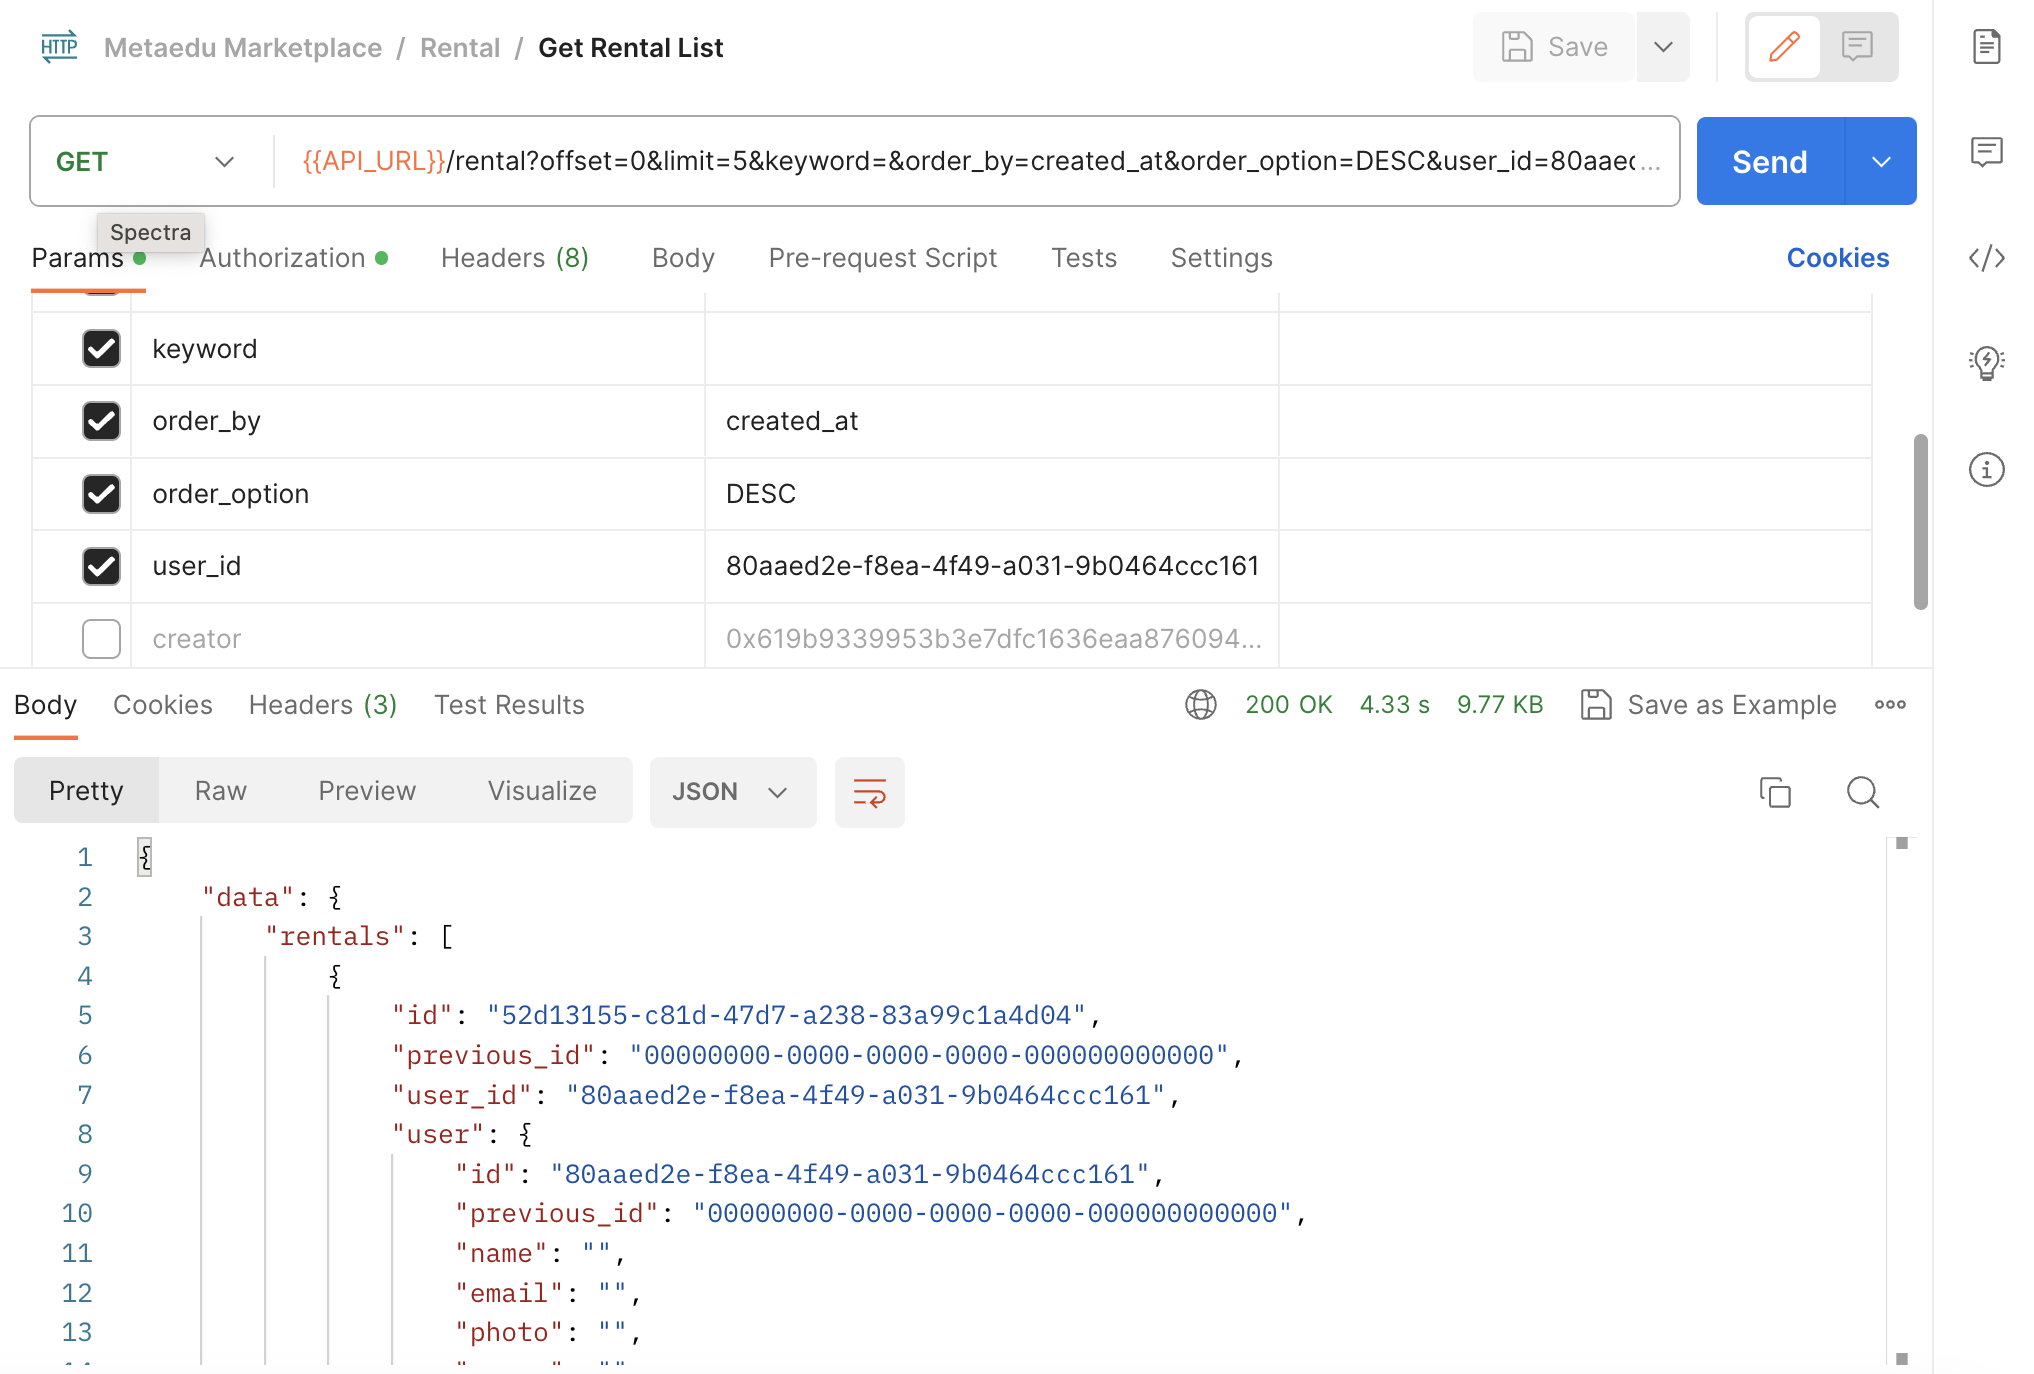
\includegraphics[scale=0.3]{gambar/img-api-rentals.png}
  \caption{\emph{API rental} }
  \label{fig:APIRentals}
\end{figure}

\emph{API} rentals memiliki \textbf{\textbackslash rental} dan digunakan memperoleh seluruh data peminjaman token yang disimpan dalam \emph{table rentals}. 

\begin{figure} [H] \centering
  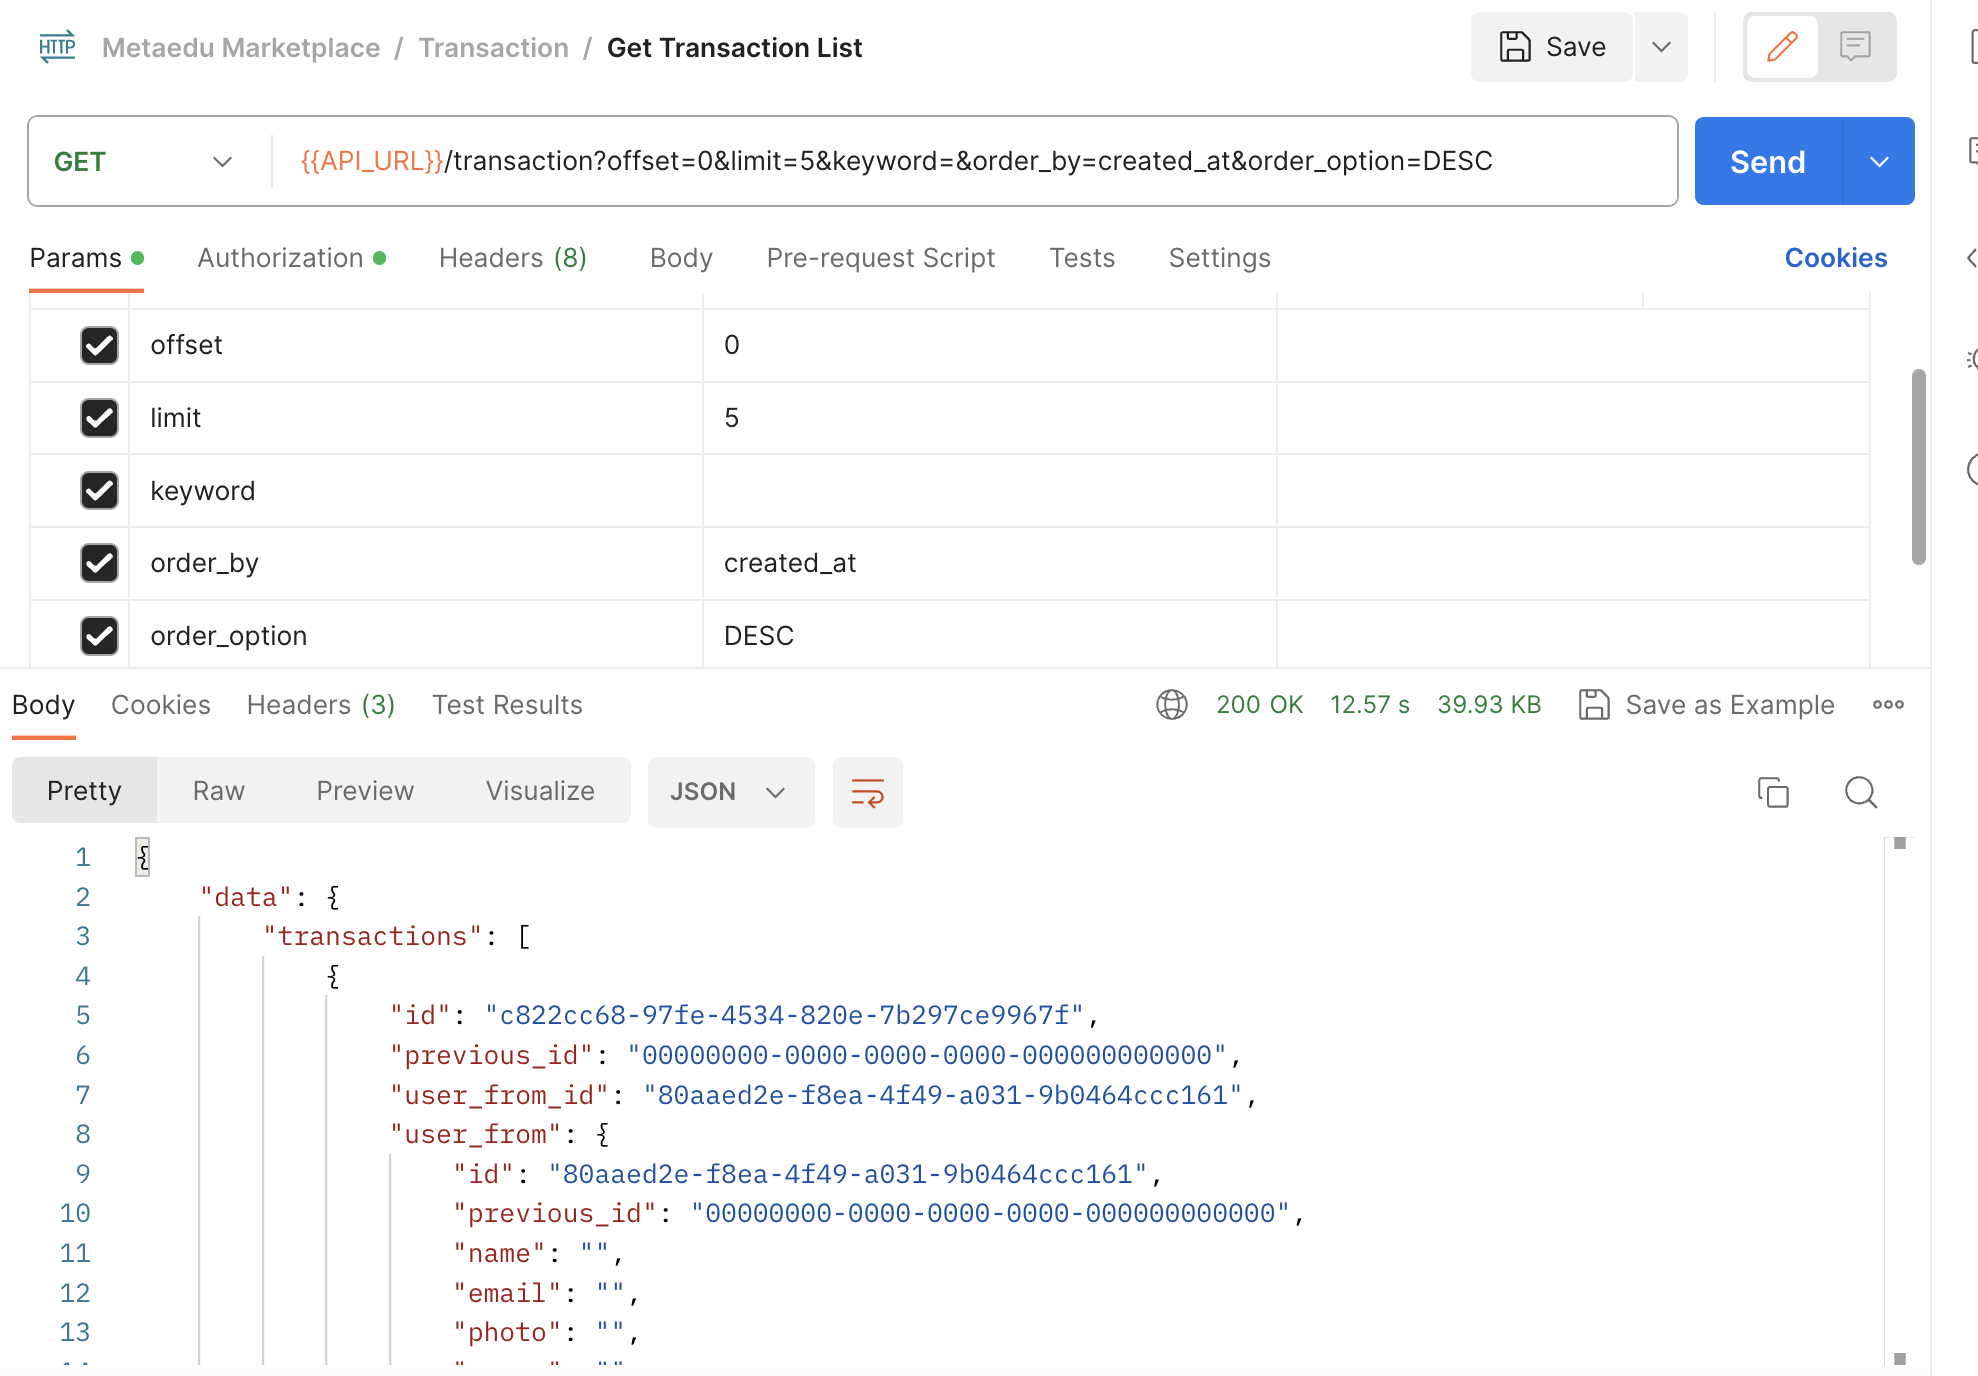
\includegraphics[scale=0.3]{gambar/img-api-transactions.png}
  \caption{\emph{API transaction} }
  \label{fig:APITransactions}
\end{figure}

\emph{API} transactions memiliki \textbf{\textbackslash transaction} dan digunakan memperoleh seluruh data transaksi baik penjualan maupun penyewaan token disimpan dalam \emph{table transactions}. 

\begin{figure} [H] \centering
  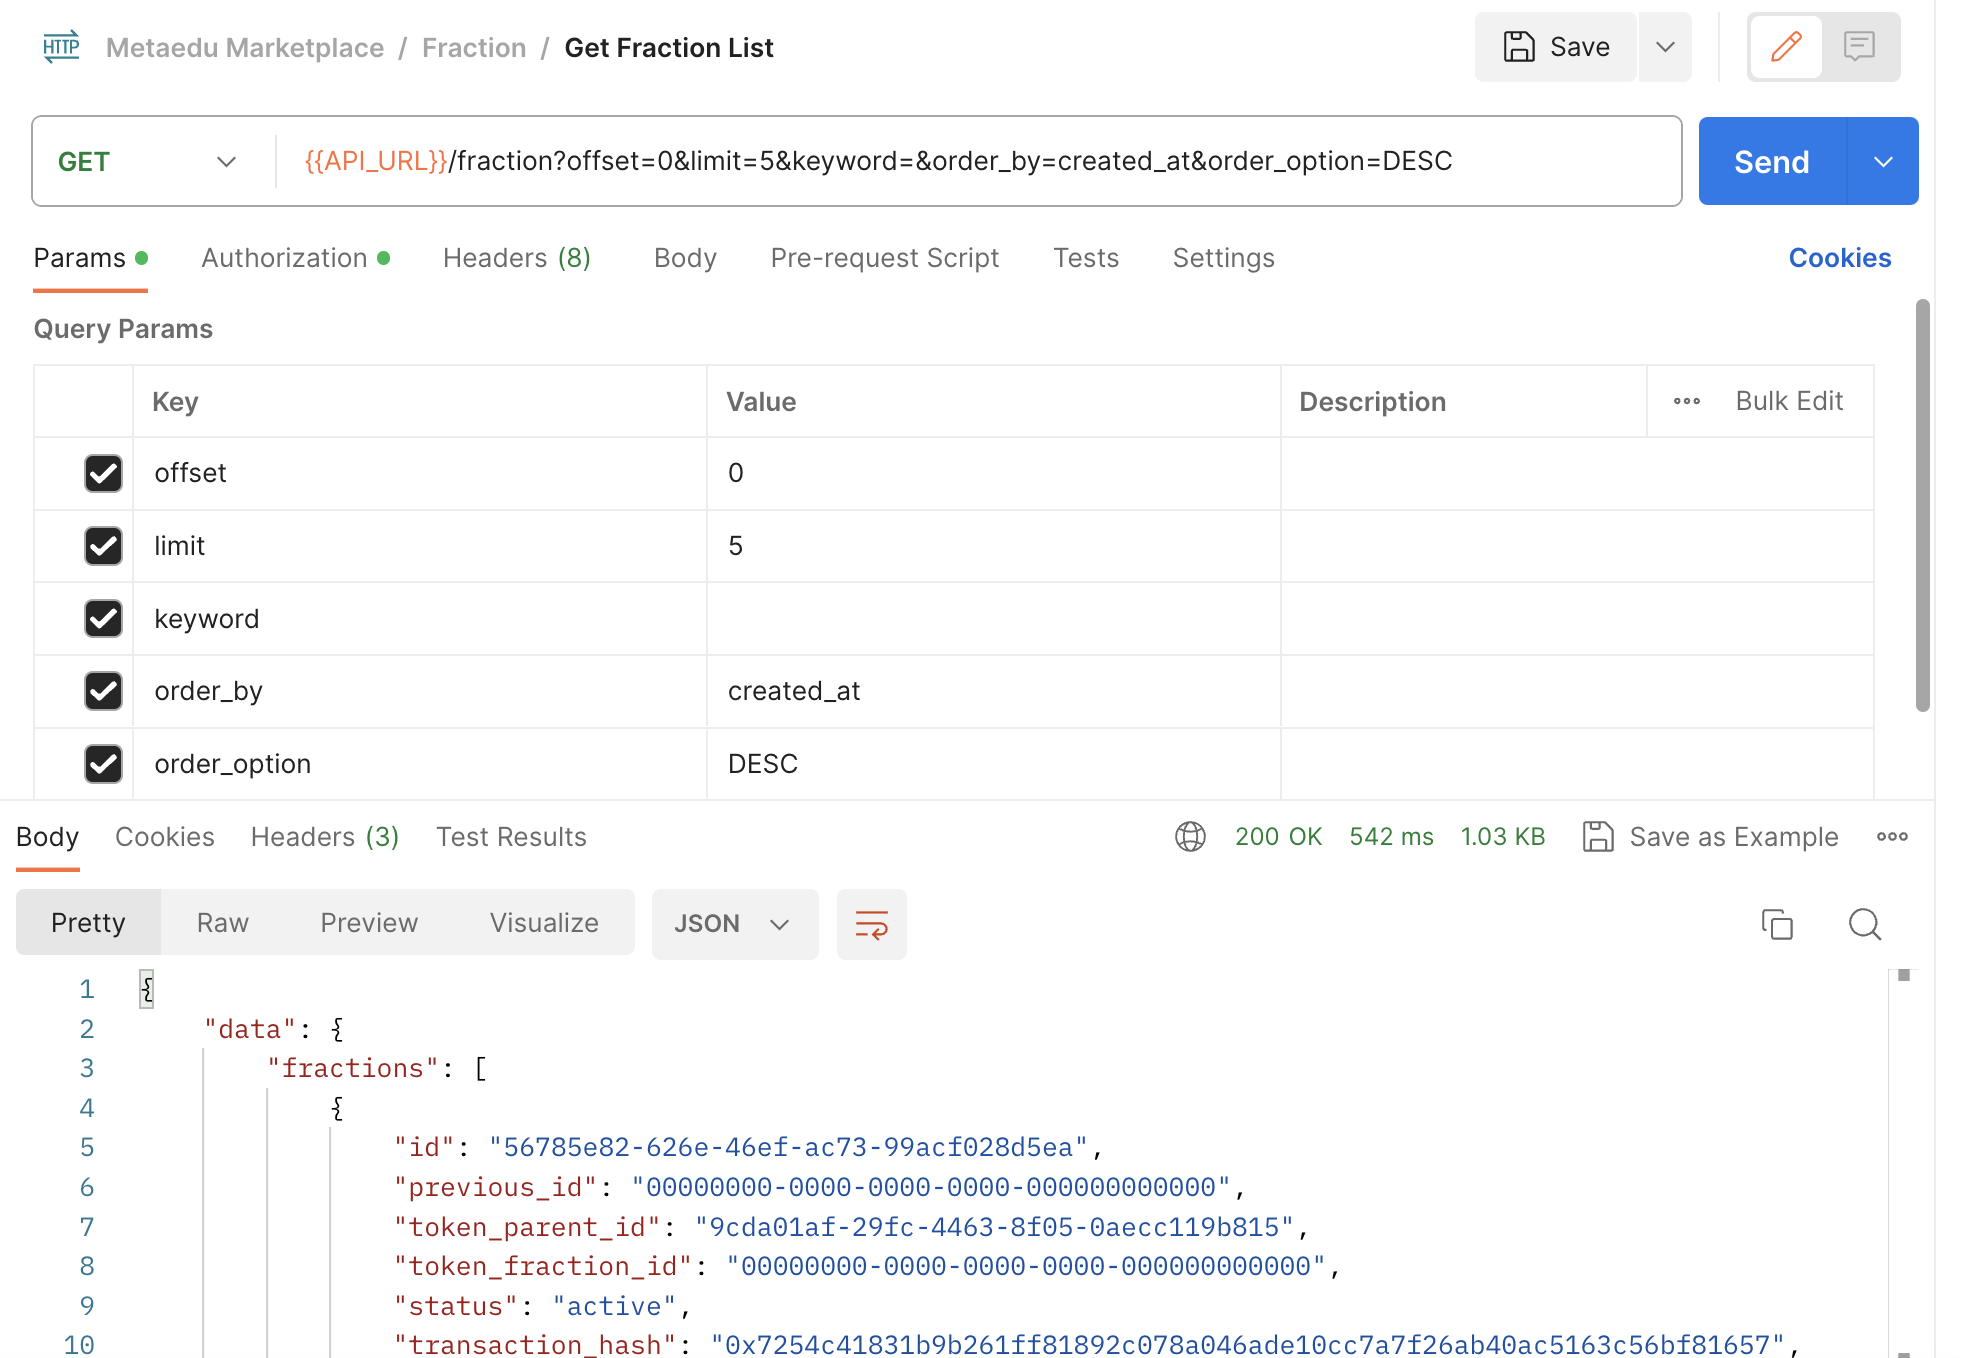
\includegraphics[scale=0.3]{gambar/img-api-fractions.png}
  \caption{\emph{API fraction} }
  \label{fig:APIFractions}
\end{figure}

\emph{API} fractions memiliki \textbf{\textbackslash fractions} dan digunakan memperoleh seluruh data \emph{fractionslization} yang disimpan dalam \emph{table fractions}. 

\emph{API-API} di atas dikembangkan supaya dapat diakses se-fleksibel mungkin sehingga menyesuaikan kebutuhan dari aplikasi \emph{frontend} dan \emph{platform metaverse} yang ingin terintegrasi. Dikarenakan hal tersebut terdapat parameter-parameter yang dapat ditambahkan dalam mengakses \emph{API} tersebut sebagai berikut

\begin{longtable}{|c|c|}
  \caption{Parameter \emph{API}}
  \label{tb:APIParameters}                                   \\
  \hline
  \rowcolor[HTML]{C0C0C0}
  \textbf{Parameter} &  \textbf{Deskripsi} \\
  \hline
  Keyword            & Memfilter data Berdasarkan kunci dari tertentu                                        \\
  Offset             & Menampilkan data dari index tertentu                           \\
  Limit            & Membatasi data                                                           \\
  Order By            & Mengurutkan data berdasarkan \emph{field} tertentu                                 \\
  Order Option        & Mengurutkan data berdasarkan index rendah ke tinggi atau sebaliknya                              \\
  Creator              & Memfilter data berdasarkan \emph{address} pemilik atau penyewa \emph{token}                                                                             \\
  User          & Memfilter data berdasarkan \emph{address} pengguna \\
  
  \hline
\end{longtable}


Pada penelitian ini dipaparkan hasil pengujian melalui aplikasi \emph{Front End} yang memicu pemanggilan \emph{function}-\emph{function} dalam \emph{smart contract}. Hasil dari pengujian ini diharapkan bahwa data-data berupa \emph{token}, \emph{ownership}, \emph{rental} sesuai dengan \emph{flow}-nya. \emph{Ether} yang dikirimkan sesuai dengan \emph{EOA} terkait transaksi tertentu sesuai. Selain itu selama pengujian berlangsung \emph{gass fee} yang diestimasikan dan diperlukan akan di data untuk mengetahui masing-masing \emph{gass fee} pada masing-masing pemanggilan \emph{function}. Hal ini menjadi penting dikarenakan merupakan suatu kondisi yang merepresentasikan bahwa \emph{smart contract} yang dikembangkan efisien.

\section{Pengujian Fitur-Fitur Utama Marketplace}
\label{sec:skenariopengujian}

Pengujian ini berfokus terhadap fitur-fitur utama pada \emph{marketplace} dalam 3 \emph{flow} yaitu pembelian, penyewaan, pembagian kepemilikan dimana yang menjadi fokus utama adalah kepemilikan NFT setelah setiap transaksi dilakukan, ketuntungan maupuan potongan yang dihasilkan selama transaksi berlangsung dan efektifias fungsi melalui gas yang dihasilkan.  \emph{Wallet} yang digunakan dalam pengujian ini adalah \emph{wallet} yang disedikan dalam \emph{environment} \emph{Hardhat}. Setiap pengujian akan menggunakan \emph{wallet} baru yang memiliki saldo 1000 \emph{ETH}.

\subsection{Pengujian \emph{Flow} Pembelian}

Ekspektasi dari pengujian \emph{flow} pembelian antara lain adalah sebagai berikut:
\begin{itemize}
    \item Antara \emph{user} dapat melakukan transaksi jual beli \emph{token}.
    \item Saldo \emph{wallet} penjual bertambah sesuai dengan harga \emph{token} yang dijual dan banyaknya \emph{token} yang dijual.
    \item Saldo \emph{wallet} pembeli berkurang sesuai dengan harga \emph{token} yang dibeli dan banyaknya \emph{token} yang dijual.
    \item Kepemilikan \emph{token} berpindah ke pembeli
    \item Seluruh data terkait dengan kepemilikan dan penjualan dari \emph{token} di halaman web sesuai dengan alur pengujian  
\end{itemize}

Berikut merupakan data mengenai \emph{wallet} yang digunakan dalam pengujian:

\begin{longtable}{|c|c|c|}
    \caption{Kondisi awal akun pada pengujian pembelian}
    \label{tb:KondisiAwalPengujianPembelian}                                   \\
    \hline
    \rowcolor[HTML]{C0C0C0}
    \textbf{\emph{Akun}} & \textbf{\emph{Address}} & \textbf{Saldo (\emph{ETH})}\\
    \hline
    A & 0x70997970C51812dc3A010C7d01b50e0d17dc79C8            & 10000               \\
    B & 0xdD2FD4581271e230360230F9337D5c0430Bf44C0            & 10000               \\
    \hline
  \end{longtable}

Berikut merupakan langkah-langkah pengujian yang akan dilakukan:
\begin{itemize}
    \item Akun A melakukan \emph{minting token} dengan suplai 1 token dan harga 10 ETH.
    \begin{figure} [H] \centering
        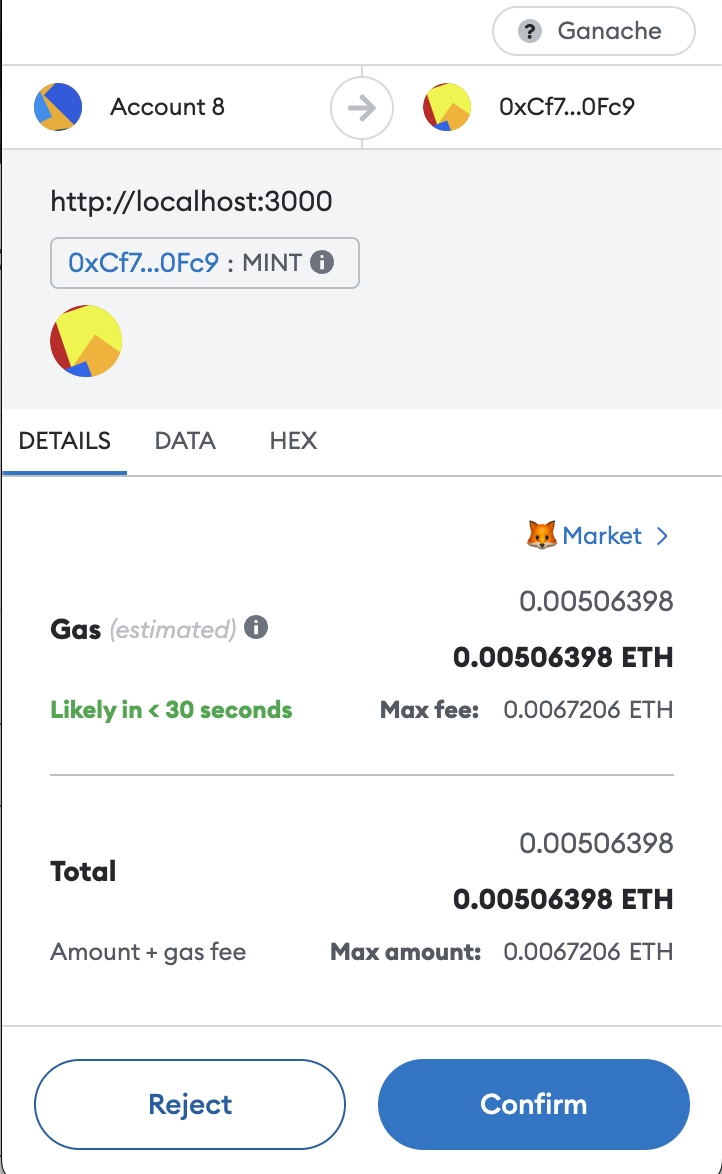
\includegraphics[scale=0.4]{gambar/img-test-buy-mint-1.png}
        \caption{Konfirmasi \emph{minting} token}
        \label{fig:TestBuyKonfirmasiMintingToken}
      \end{figure}
    Pada gambar terlihat bahwa estimasi \emph{gas} adalah \textbf{0,00506398} \emph{ETH}
    \begin{figure} [H] \centering
        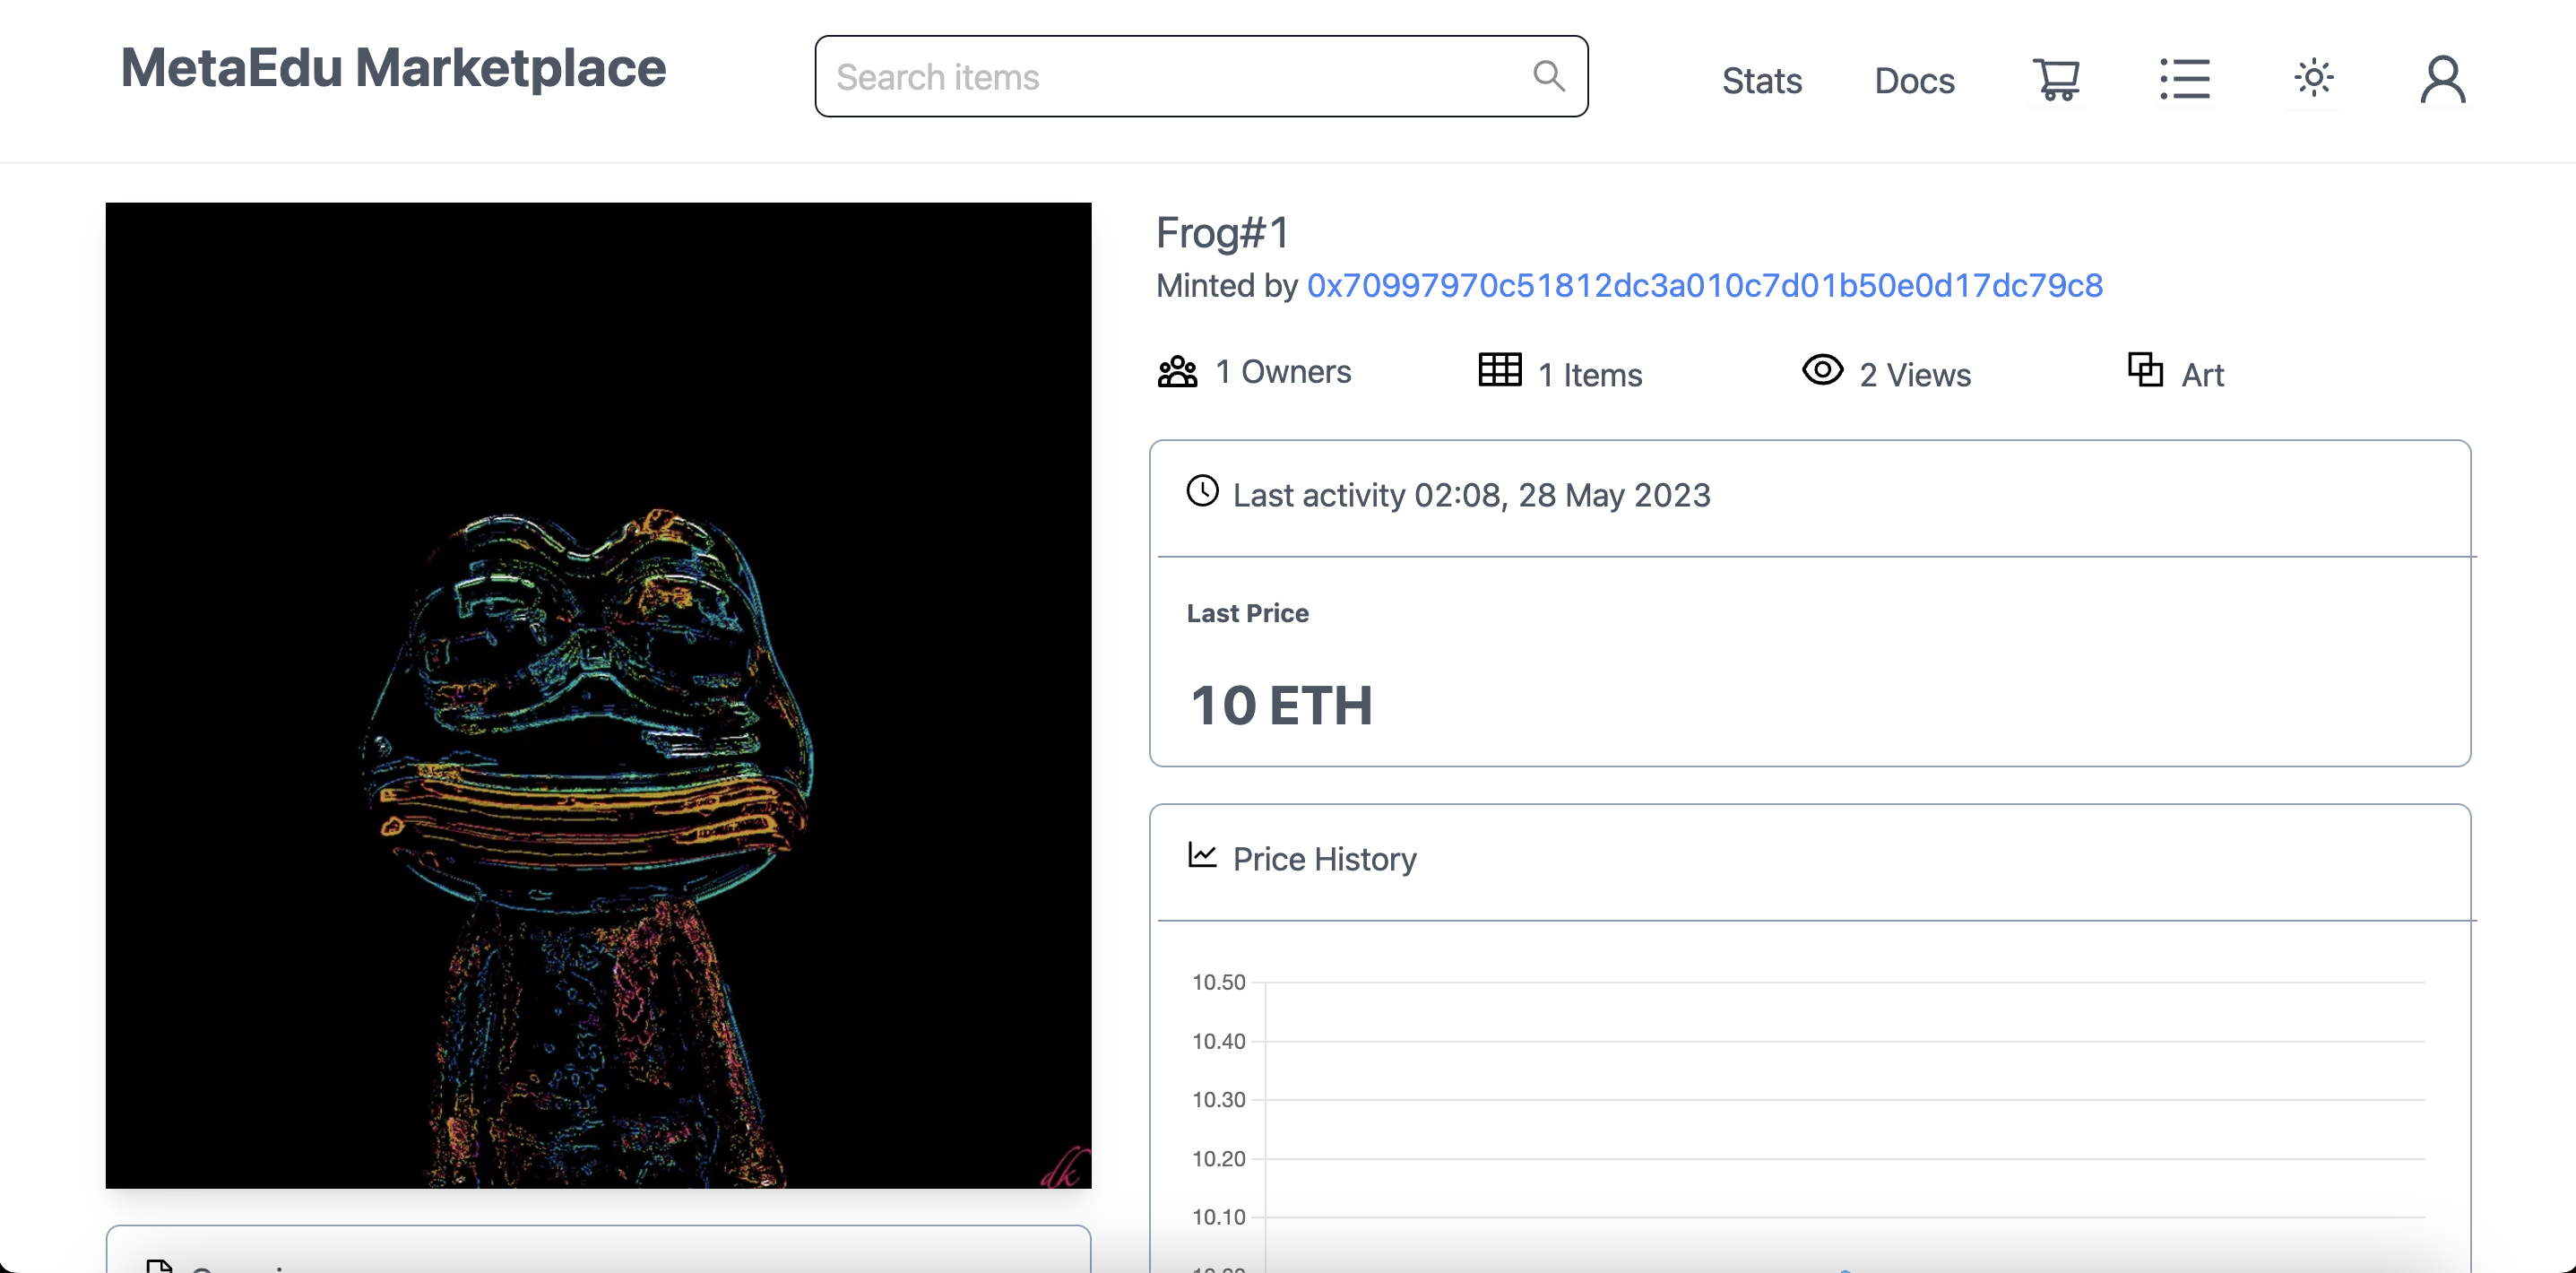
\includegraphics[scale=0.3]{gambar/img-test-buy-mint-2.png}
        \caption{Hasil minting token-1}
        \label{fig:TestBuyHasilMinting}
      \end{figure}
      \begin{figure} [H] \centering
        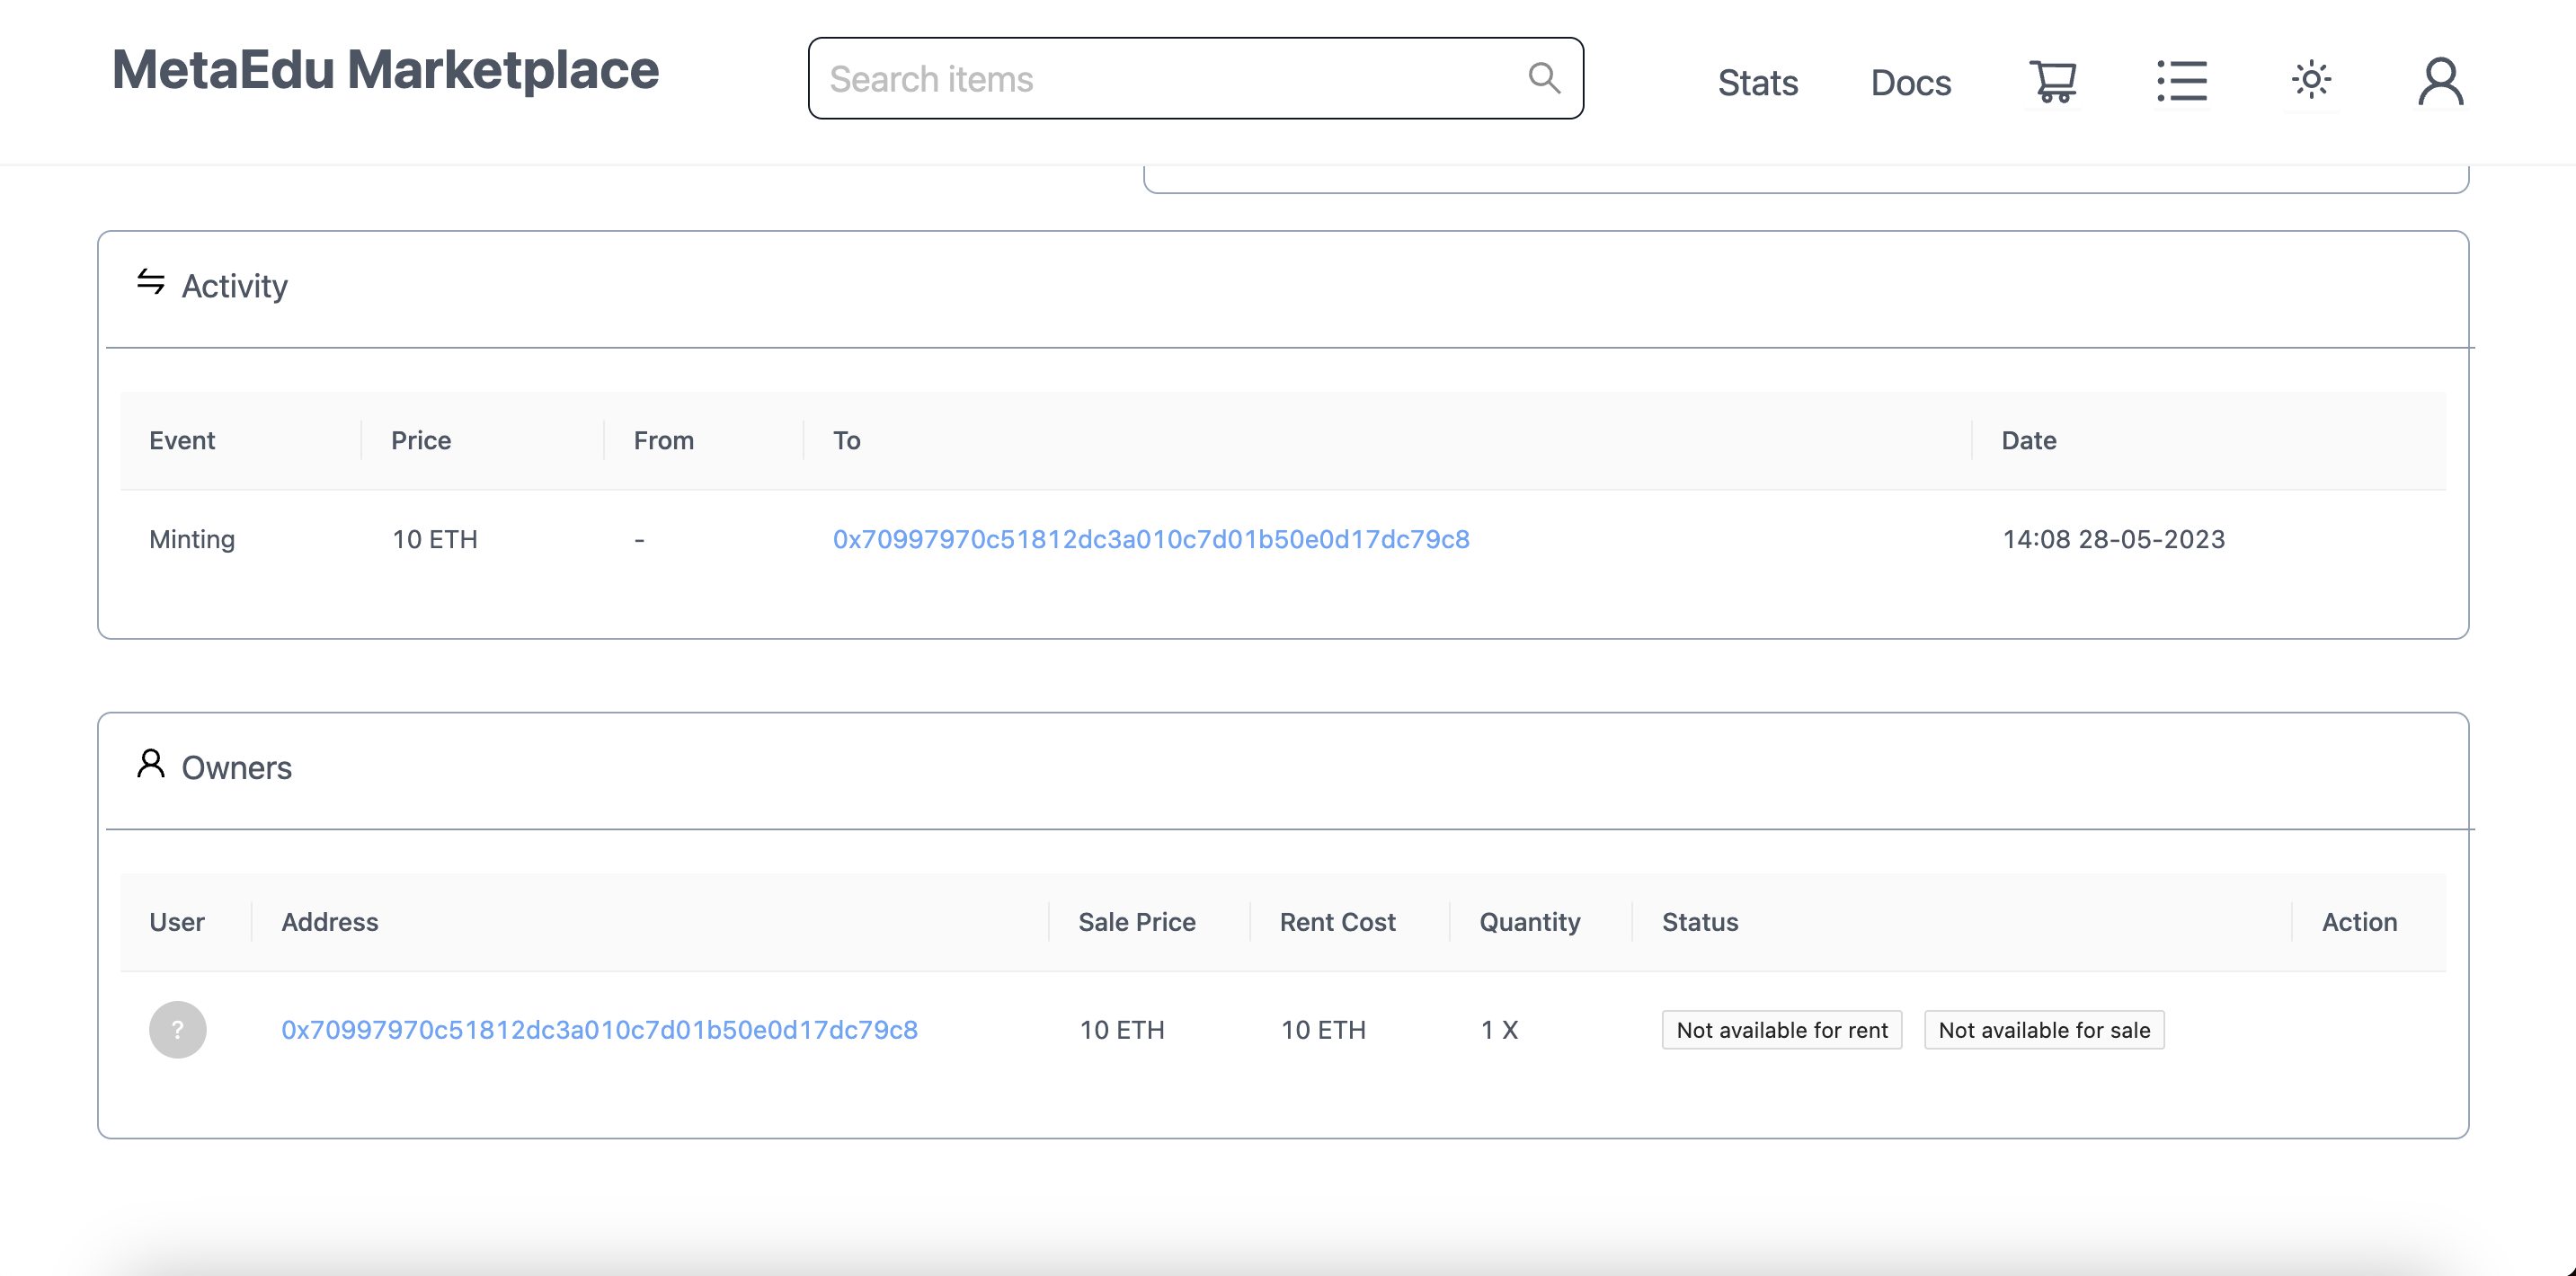
\includegraphics[scale=0.3]{gambar/img-test-buy-mint-3.png}
        \caption{Hasil minting token-2}
        \label{fig:TestBuyHasilMinting}
      \end{figure}
      \begin{figure} [H] \centering
        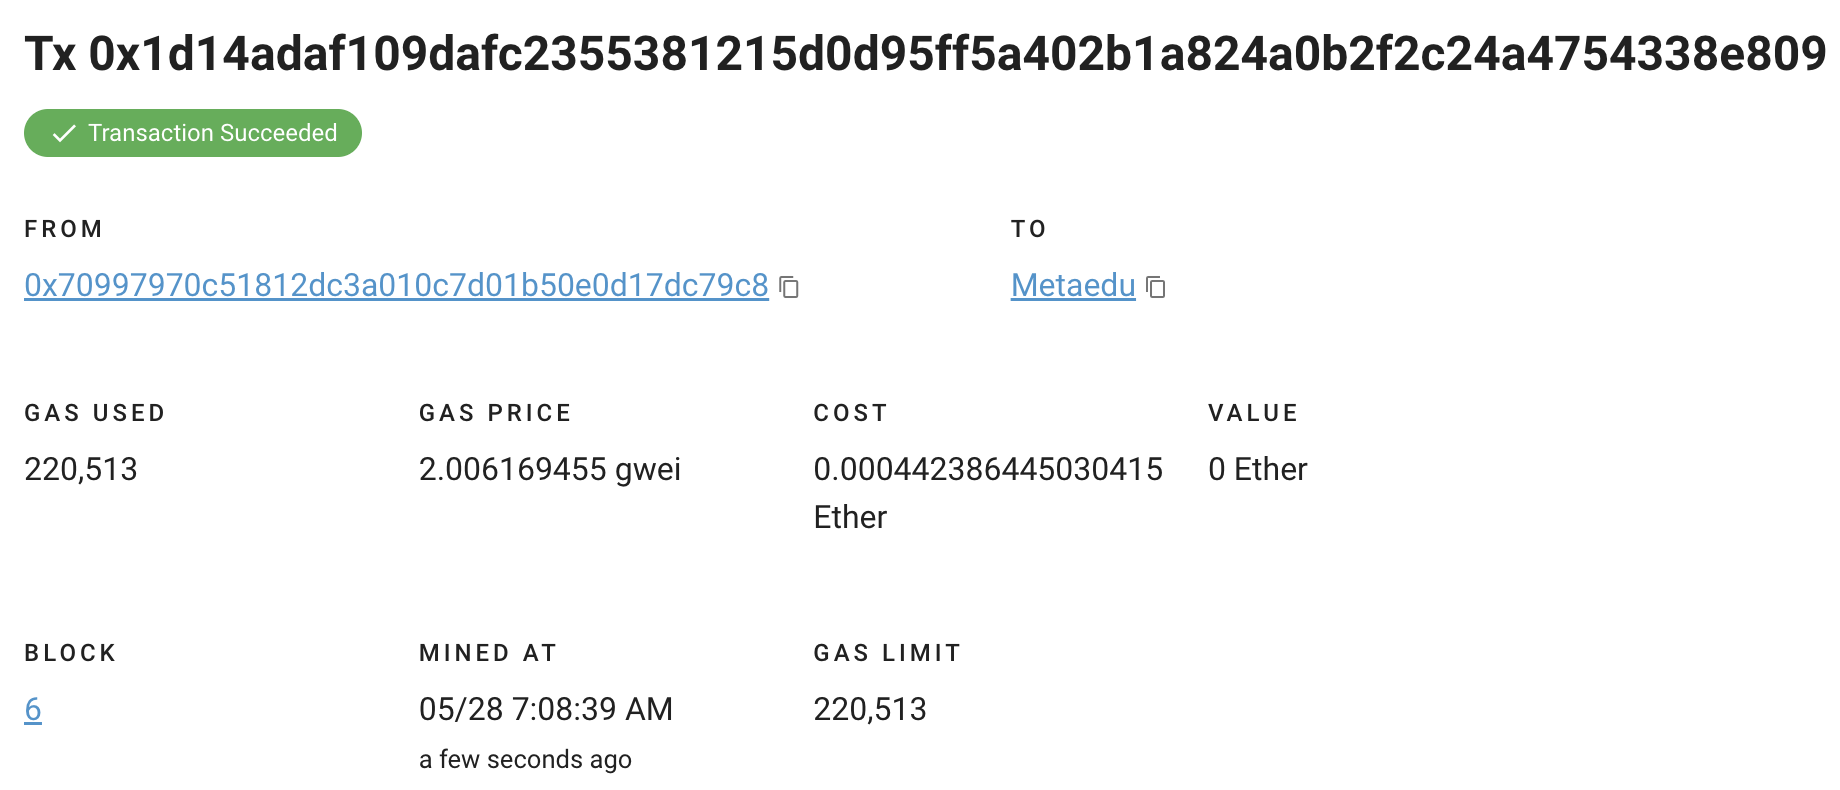
\includegraphics[scale=0.4]{gambar/img-test-buy-mint-4.png}
        \caption{Hasil minting token pada \emph{Ethernal}}
        \label{fig:TestBuyHasilMinting}
      \end{figure}
    Pada gambar dapat diketahui bahwa \emph{gas} yang diperlukan/\emph{gas used} adalah \textbf{220,513} dan \emph{gas price} adalah \textbf{2,006169455} \emph{gwei} maka \emph{gas fee} yang dibayarkan adalah \textbf{0,000442386445030415} \emph{ETH}
    \item Akun A memperbarui status token yang telah di-\emph{minting} supaya dapat dijual.
    \begin{figure} [H] \centering
        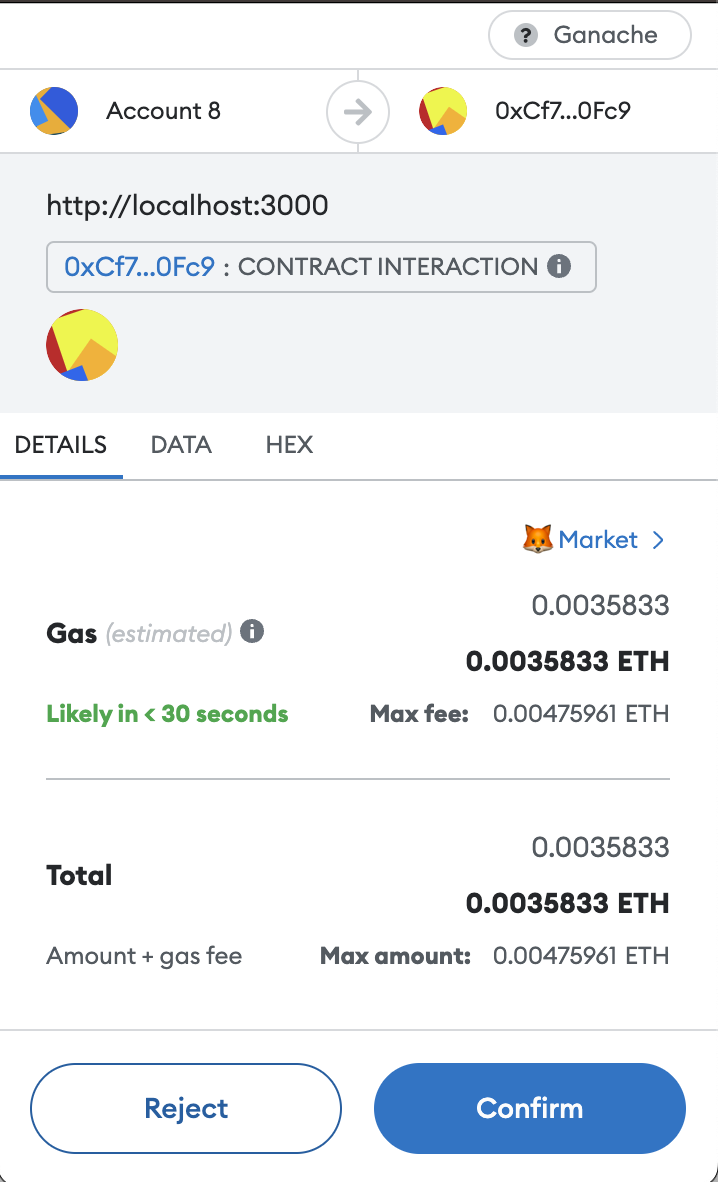
\includegraphics[scale=0.3]{gambar/img-test-buy-put-item-for-sale-1.png}
        \caption{Konfirmasi pembaruan status penjualan token}
        \label{fig:TestBuyKonfirmasiPembaruanPenjual}
      \end{figure}
      Pada gambar dapat diketahu bahwa estimasi \emph{gas fee} adalah \textbf{0,0035833 \emph{ETH}}.
      \begin{figure} [H] \centering
        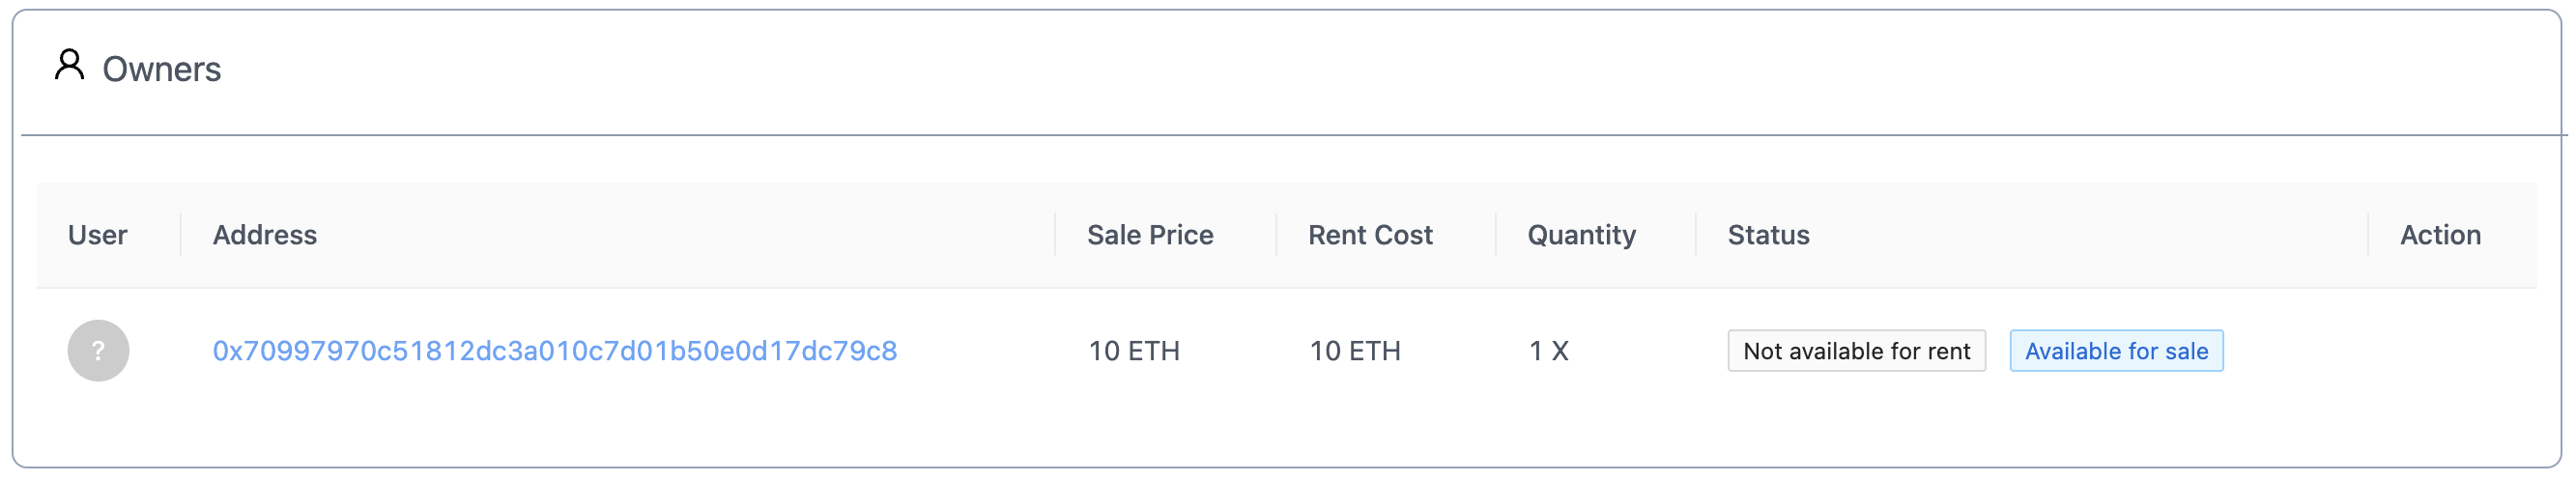
\includegraphics[scale=0.3]{gambar/img-test-buy-put-item-for-sale-2.png}
        \caption{Hasil pembaruan status penjualan \emph{token} pada \emph{web}}
        \label{fig:TestBuyPutItemForSale}
      \end{figure}
      \begin{figure} [H] \centering
        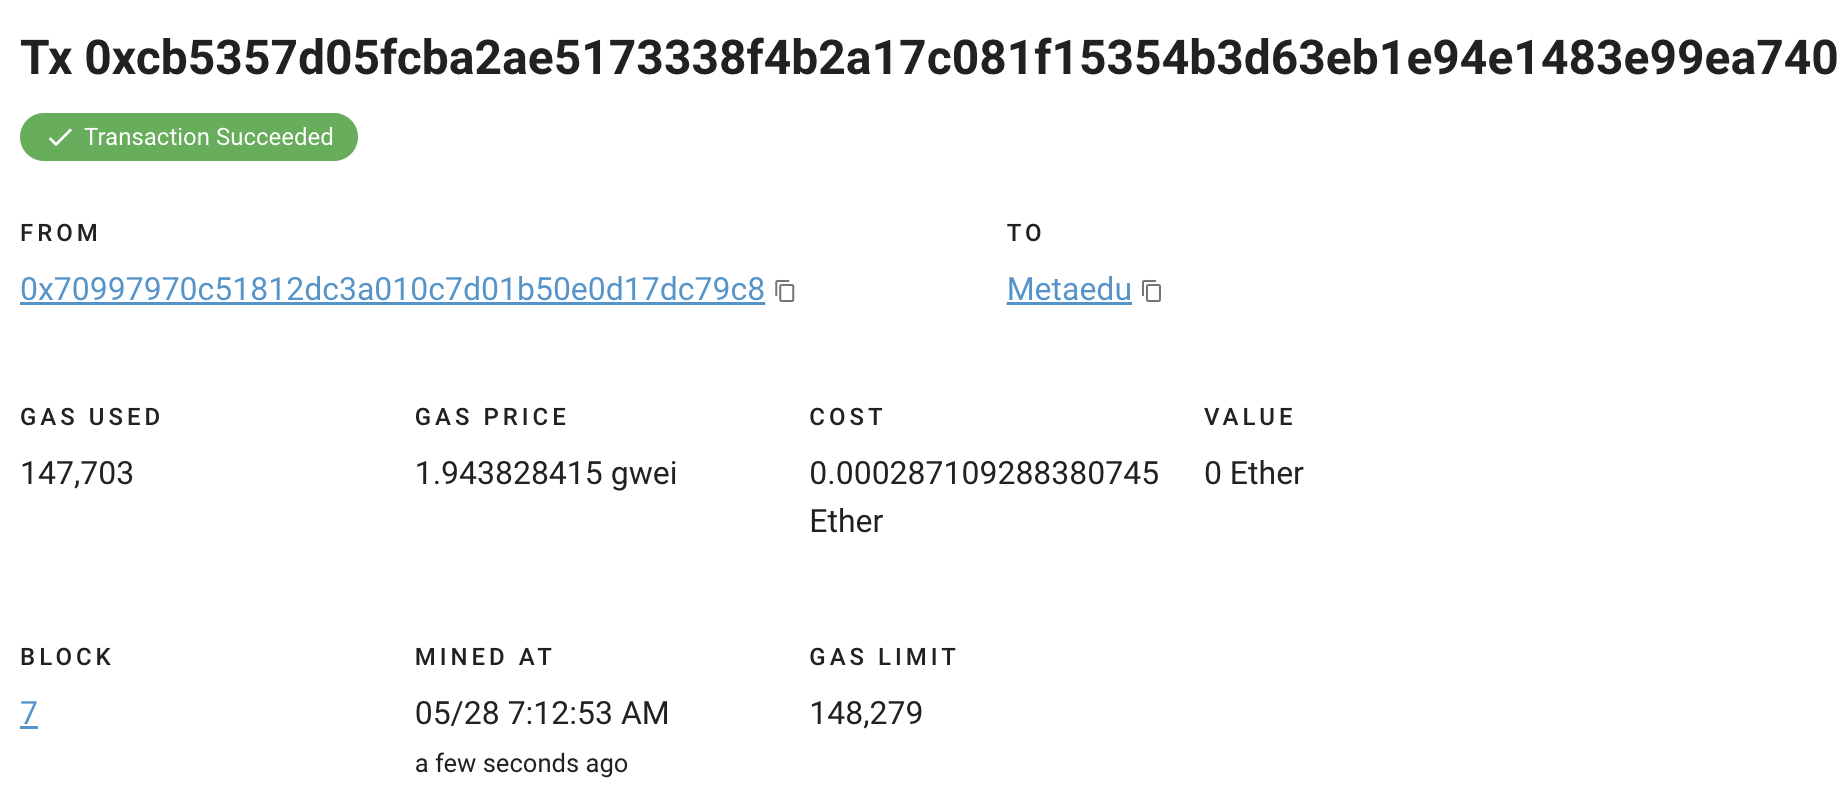
\includegraphics[scale=0.3]{gambar/img-test-buy-put-item-for-sale-4.png}
        \caption{Hasil pembaruan status penjualan \emph{token} pada \emph{Ethernal}}
        \label{fig:TestBuyPutItemForSaleEthernal}
      \end{figure}
      Pada gambar dapat diketahui bahwa \emph{gas} yang diperlukan/\emph{gas used} adalah \textbf{147,703} dan \emph{gas price} adalah \textbf{1,943828415 \emph{gwei}} maka \emph{gas fee} yang dibayarkan adalah \textbf{0,000287109288380745 \emph{ETH}}.
    \item Akun B membeli \emph{token} yang dimiliki oleh akun A
    \begin{figure} [H] \centering
        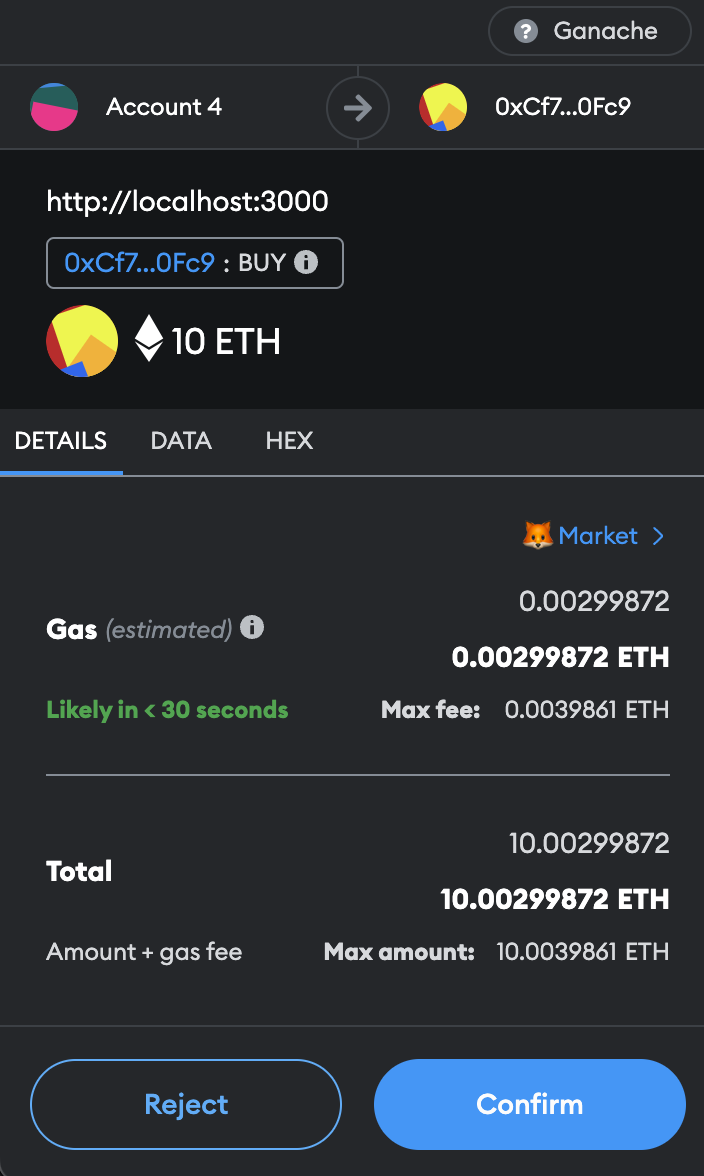
\includegraphics[scale=0.4]{gambar/img-test-buy-buy-1.png}
        \caption{Konfirmasi pembelian token}
        \label{fig:TestBuyKonfirmasiPembelianToken}
      \end{figure}
    Pada gambar dapat diketahui bahwa estimasi \emph{gas} adalah \textbf{0,00299872 \emph{ETH}} dan harga pembelian adalah \textbf{10 ETH} sesuai dengan harga jual \emph{token}
    \begin{figure} [H] \centering
        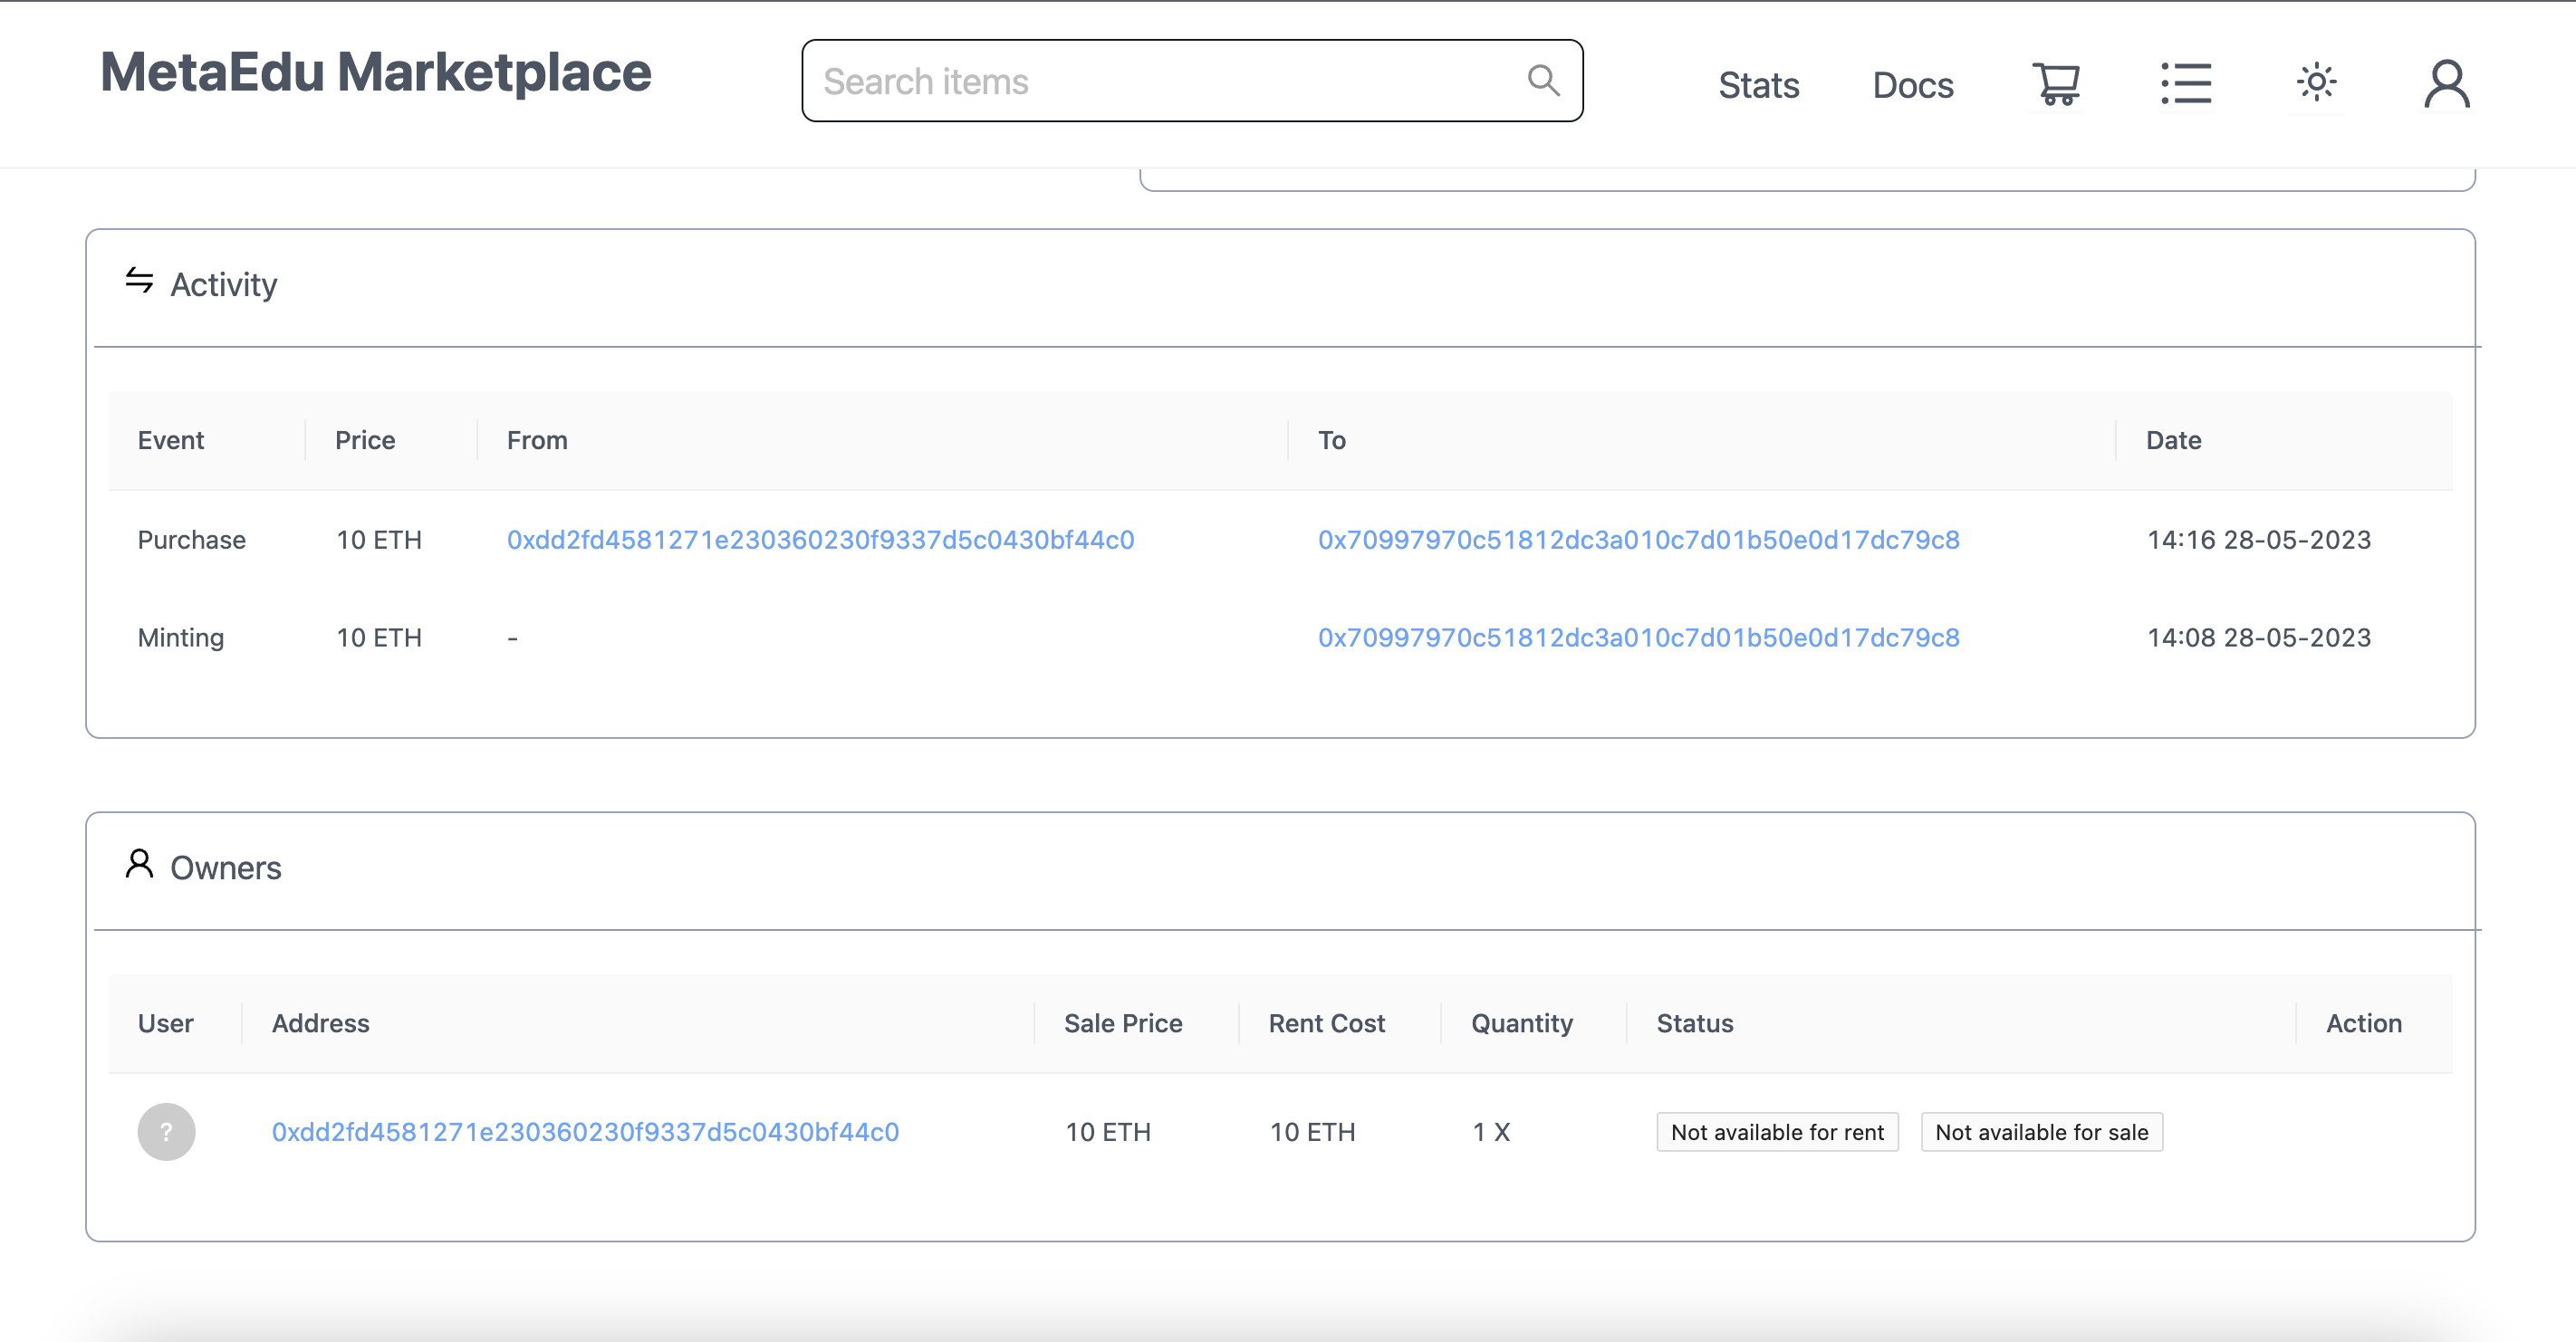
\includegraphics[scale=0.3]{gambar/img-test-buy-buy-2.png}
        \caption{Hasil pembelian token}
        \label{fig:TestBuyHasilPembelian}
      \end{figure}
      Setelah dilakukan pembelian maka \emph{address} \emph{owner} akan menjadi \emph{address} dari akun B dan data pembelian akan tercatat pada tabel \emph{activity}.
      \begin{figure} [H] \centering
        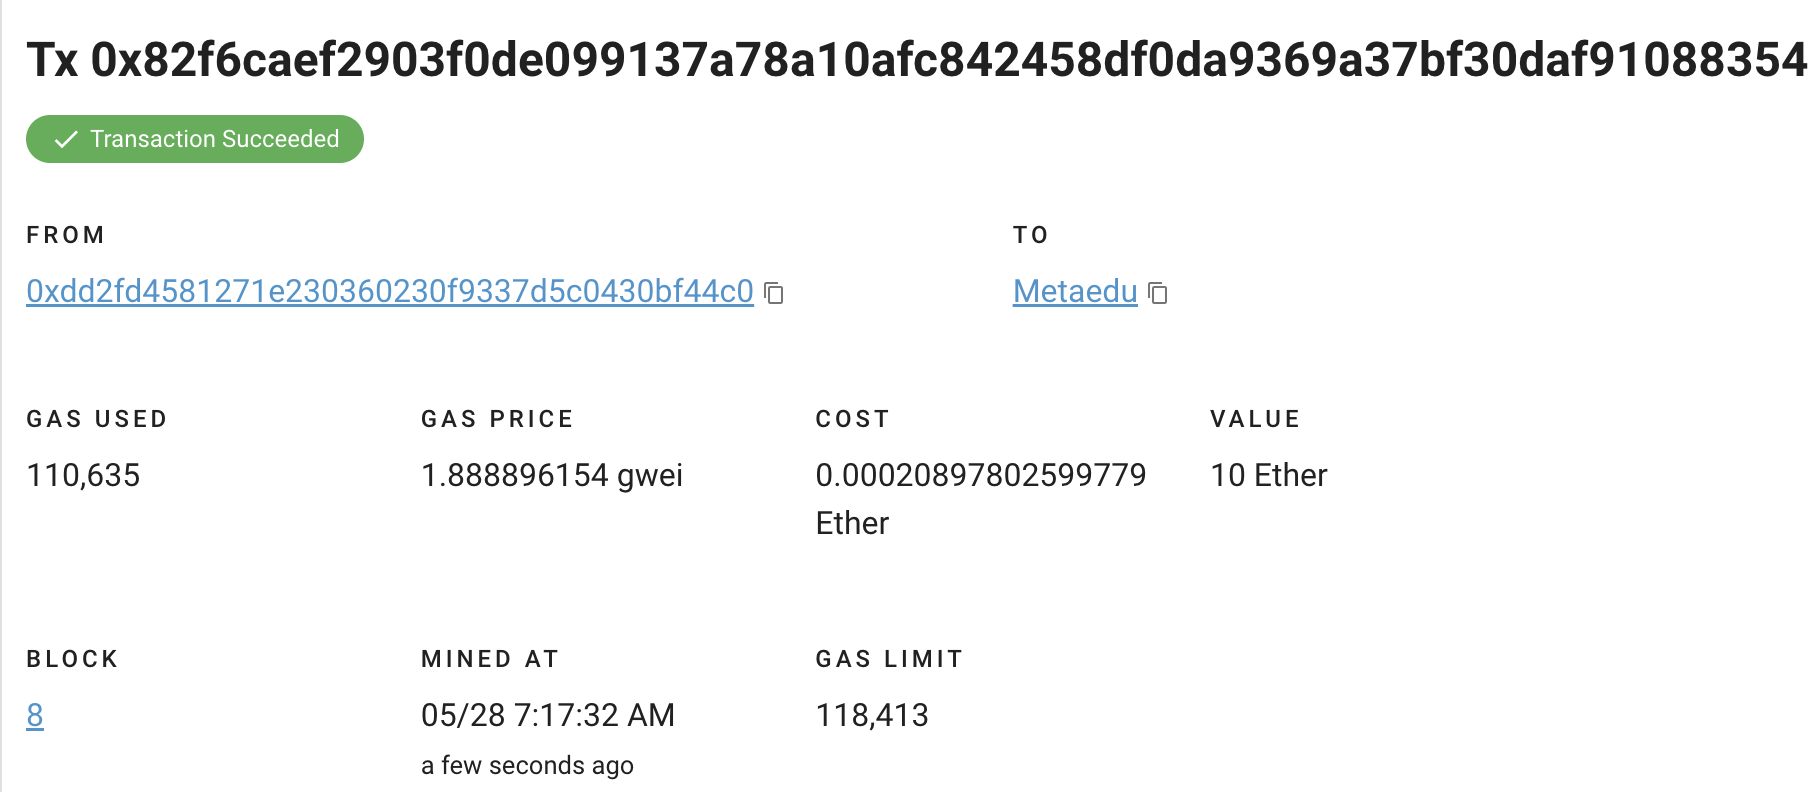
\includegraphics[scale=0.4]{gambar/img-test-buy-buy-5.png}
        \caption{Hasil pembelian token pada \emph{Ethernal}}
        \label{fig:TestBuyHasilPembelian2}
      \end{figure}
      Pada gambar dapat diketahui bahwa \emph{gas} yang diperlukan/\emph{gas used} adalah \textbf{110,635} dan \emph{gas price} adalah \textbf{1,888896154 \emph{gwei}} maka \emph{gas fee} yang dibayarkan adalah \textbf{0.00020897802599779 \emph{ETH}}.
    \begin{figure} [H] \centering
        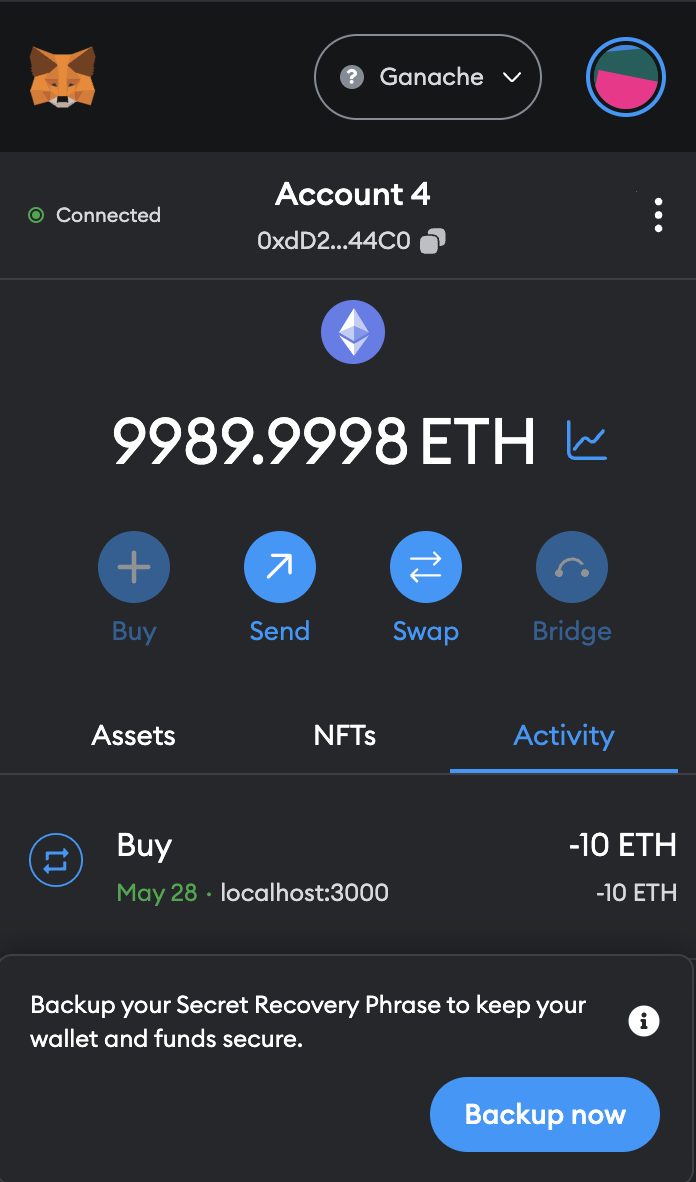
\includegraphics[scale=0.4]{gambar/img-test-buy-buy-3.png}
        \caption{Saldo akun B setelah melakukan pembelian}
        \label{fig:TestBuyHasilPembelian3}
      \end{figure}
    Saldo dari \emph{wallet} akun B berkurang sebesar \textbf{10 \emph{ETH}} ditambah dengan \emph{gas fee} yang diperlukan pada transaksi sebelumnya menjadi 9989.9998 \emph{ETH}.
    \begin{figure} [H] \centering
        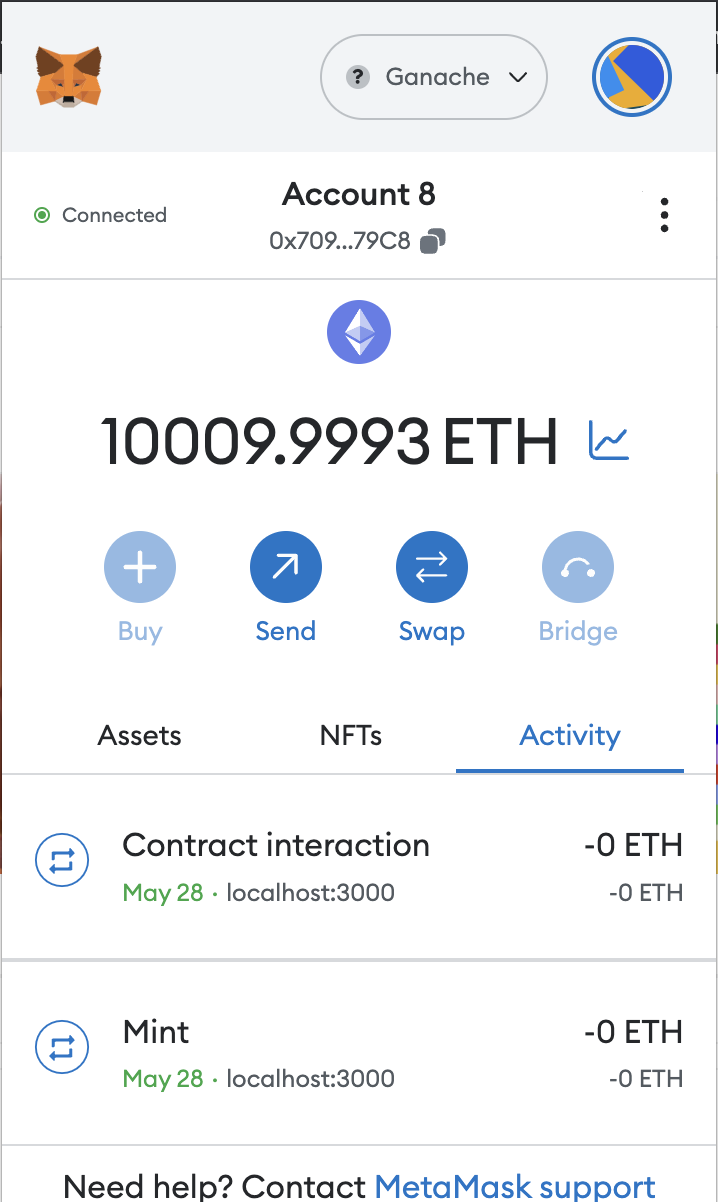
\includegraphics[scale=0.4]{gambar/img-test-buy-buy-4.png}
        \caption{Saldo akun A bertambah setelah token yang dimiliki dibeli}
        \label{fig:TestBuyHasilPembelian4}
      \end{figure}
    Saldo dari \emph{wallet} akun A bertambah sebesar \textbf{10 \emph{ETH}} ditambah dengan \emph{gas fee} yang diperlukan pada transaksi sebelumnya menjadi 9989.9998 \emph{ETH}. 
\end{itemize}

Setelah dilakukan pengujian pembelian maka dapat diketahui bahwa alur dari aplikasi telah berjalan sesuai dengan harapan pengujian yang telah disebutkan di awal dimana salah satunya adalah penjual memperoleh \emph{ETH} sesuai dengan harga token dan jumlah yang dijual yaitu \emph{\textbf{10 ETH}} dan sebaliknya pembeli mendapatkan potongan sebesar \emph{\textbf{10 ETH}}. Selain itu juga diperoleh data mengenai \emph{gas fee} sesuai dengan tabel berikut

\begin{longtable}{|c|c|c|c|}
    \caption{\emph{Gas fee} yang diperoleh selama pengujian \emph{flow} pembelian}
    \label{tb:EnergiKecepatan}                                   \\
    \hline
    \rowcolor[HTML]{C0C0C0}
    \textbf{\emph{Function}}  & \textbf{\emph{Gas used}} & \textbf{\emph{Gas price}}  & \textbf{\emph{Gas fee} yang dibayarkan (\emph{ETH})} \\
    \hline
    \emph{mint}           & 220,513 & 2,006169455  & 0,000442386445030415    \\
    \emph{putItemForSale} & 147,703 & 1,943828415  & 0,000287109288380745    \\
    \emph{buy}            & 110,635 & 1.888896154  & 0.00020897802599779      \\
    \hline
  \end{longtable}

\subsection{\emph{Flow} Penyewaan}

Ekspektasi dari pengujian \emph{flow} penyewaan antara lain adalah sebagai berikut:
\begin{itemize}
    \item Pemilik \emph{token} dapat menyewakan \emph{token} yang dimiliki.
    \item Pengguna lain dapat menyewa \emph{token}.
    \item Saldo \emph{wallet} pemilik bertambah sesuai dengan harga dan lama sewa.
    \item Saldo \emph{wallet} penyewa berkurang sesuai dengan harga dan lama sewa.
    \item Seluruh data terkait dengan kepemilikan dan penyewaan dari \emph{token} di halaman web sesuai dengan alur pengujian  
\end{itemize}

Berikut merupakan data mengenai \emph{wallet} yang digunakan dalam pengujian:

\begin{longtable}{|c|c|c|}
    \caption{Kondisi awal}
    \label{tb:KondisiAwalPengujianSewa}                                   \\
    \hline
    \rowcolor[HTML]{C0C0C0}
    \textbf{\emph{Akun}} & \textbf{\emph{Address}} & \textbf{Saldo (\emph{ETH})}\\
    \hline
    A & 0xcd3B766CCDd6AE721141F452C550Ca635964ce71            & 10000               \\
    B & 0x2546BcD3c84621e976D8185a91A922aE77ECEc30            & 10000               \\
    \hline
  \end{longtable}

Berikut merupakan langkah-langkah pengujian yang akan dilakukan:
  \begin{itemize}
      \item Akun A melakukan \emph{minting token} dengan suplai 1 token dan harga 10 ETH.
      \begin{figure} [H] \centering
          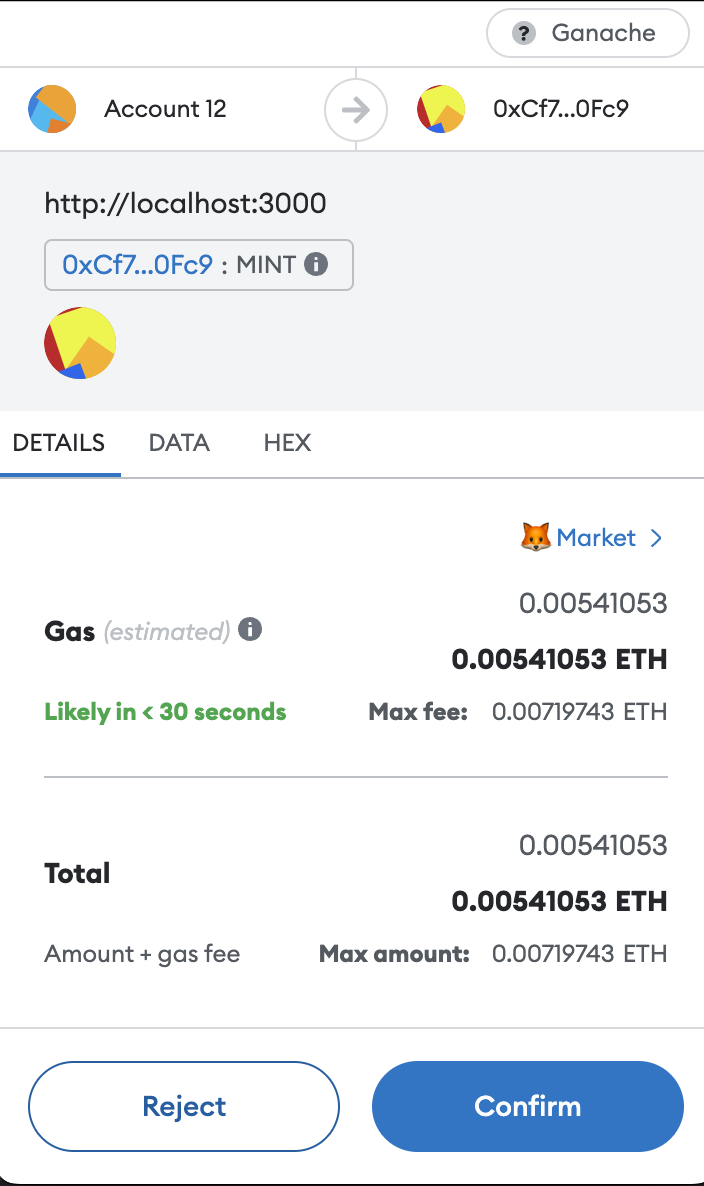
\includegraphics[scale=0.4]{gambar/img-test-rent-mint-1.png}
          \caption{Konfirmasi \emph{minting} token}
          \label{fig:TestRentKonfirmasiMintingToken}
        \end{figure}
      Pada gambar terlihat bahwa estimasi \emph{gas} adalah \textbf{0,00541053} \emph{ETH}
      \begin{figure} [H] \centering
          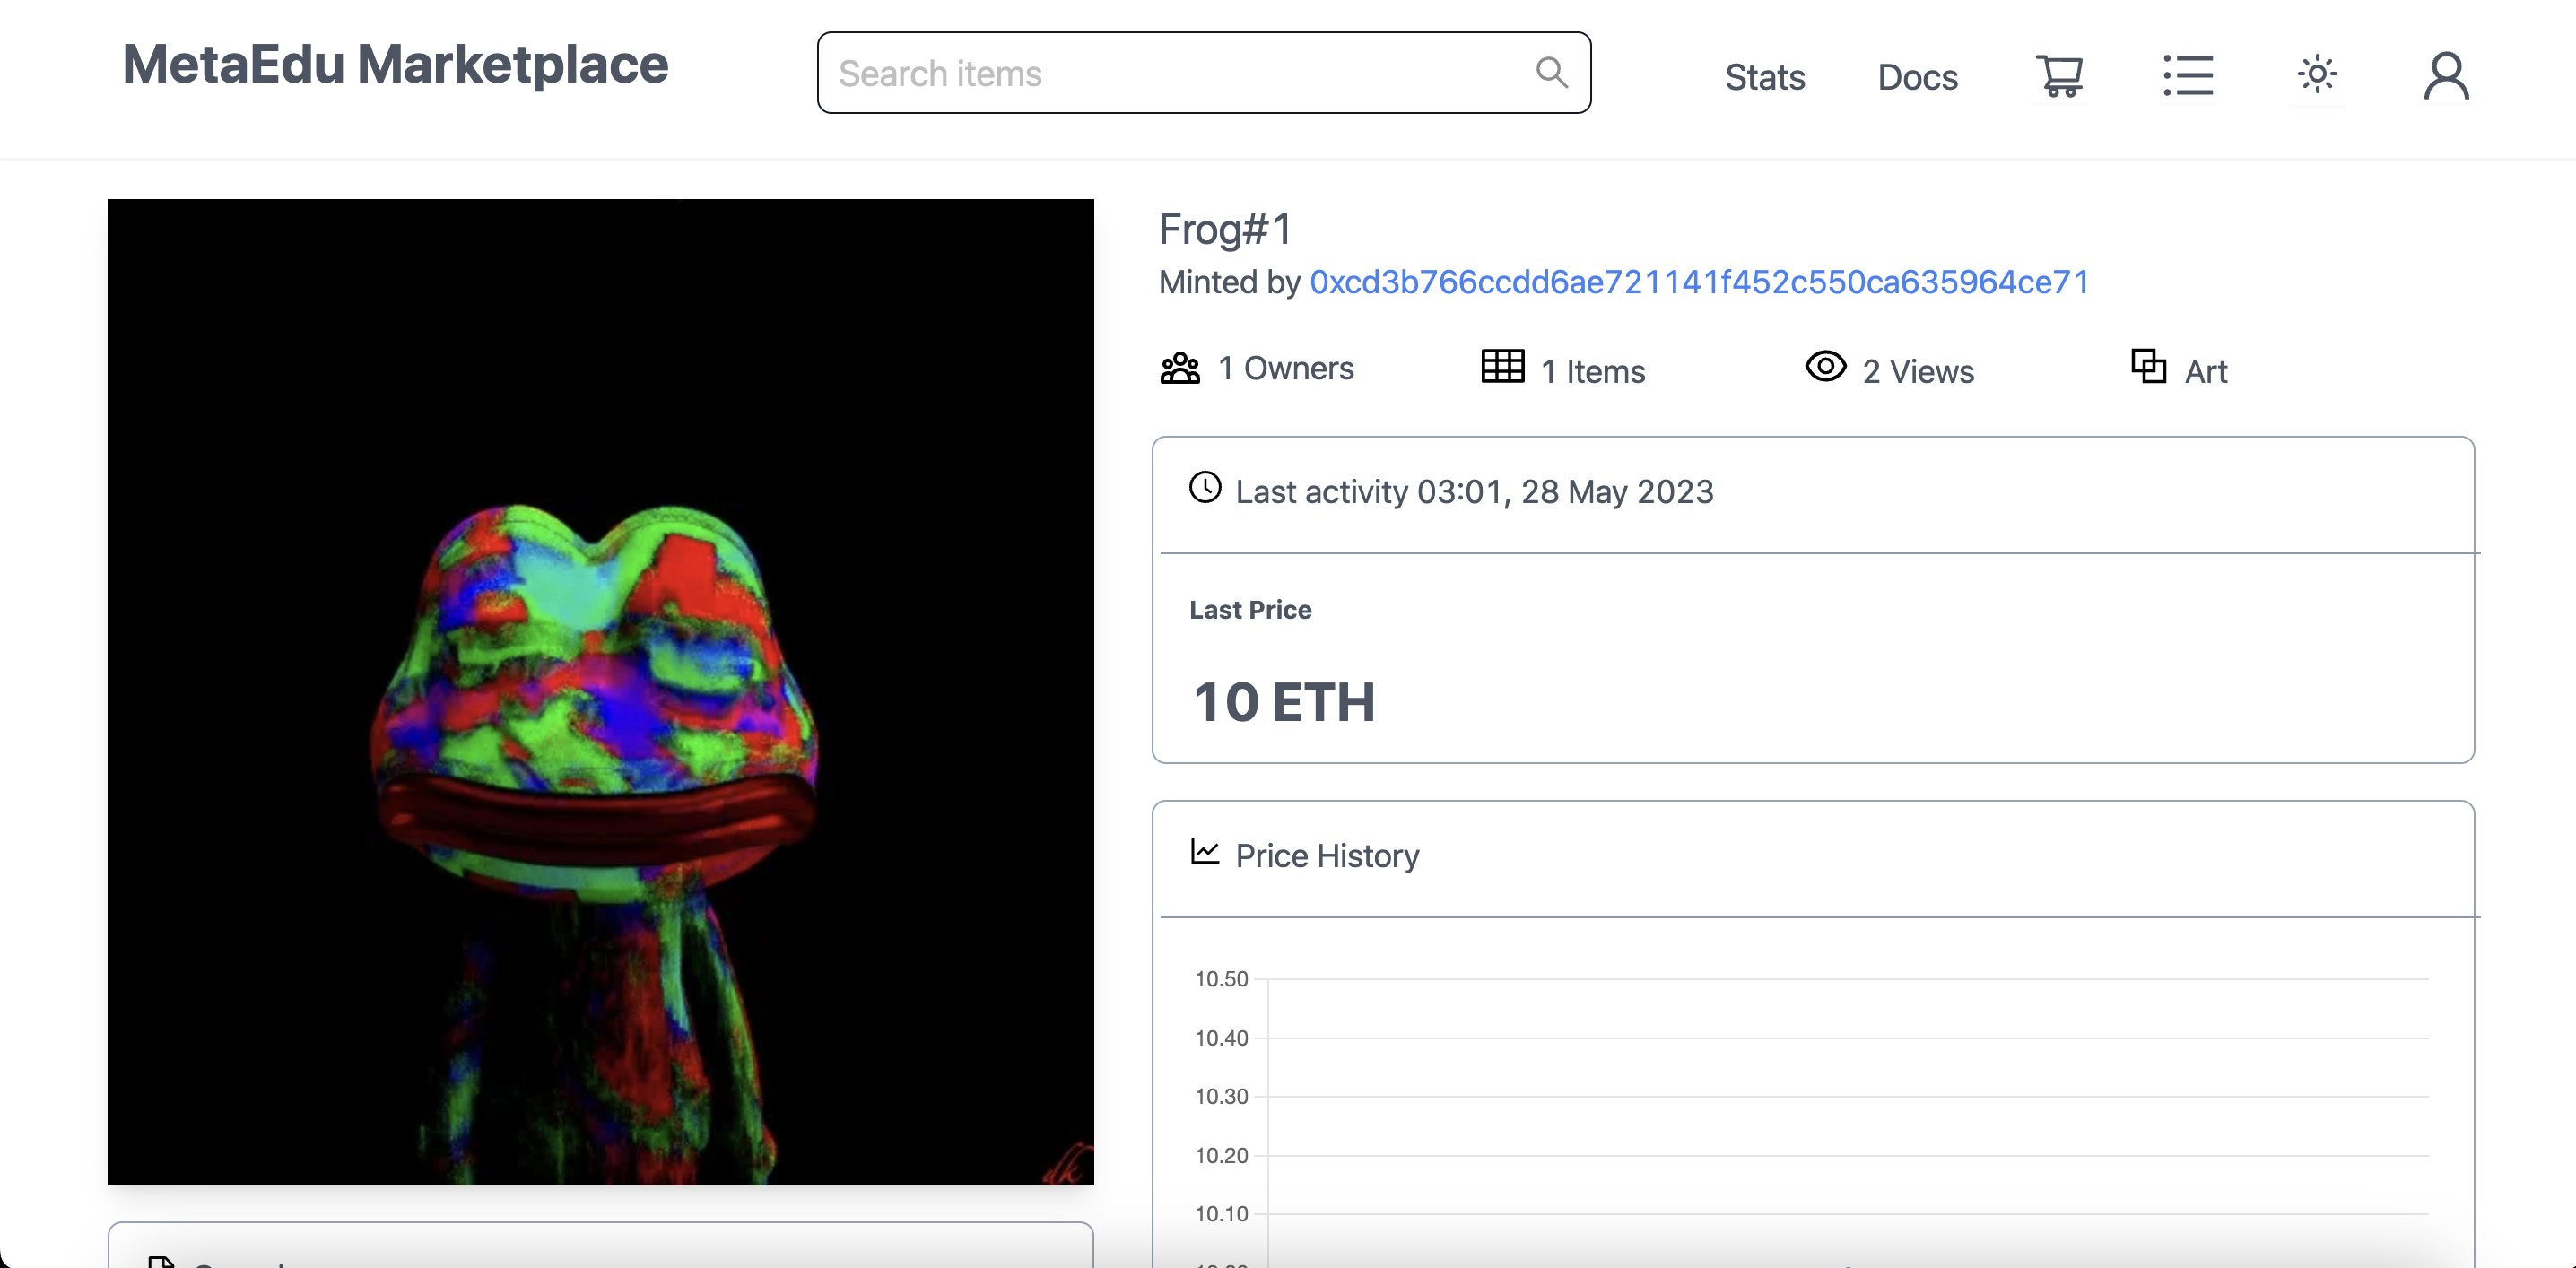
\includegraphics[scale=0.3]{gambar/img-test-rent-mint-2.png}
          \caption{Hasil minting token-1}
          \label{fig:TestRentHasilMinting}
        \end{figure}
        \begin{figure} [H] \centering
          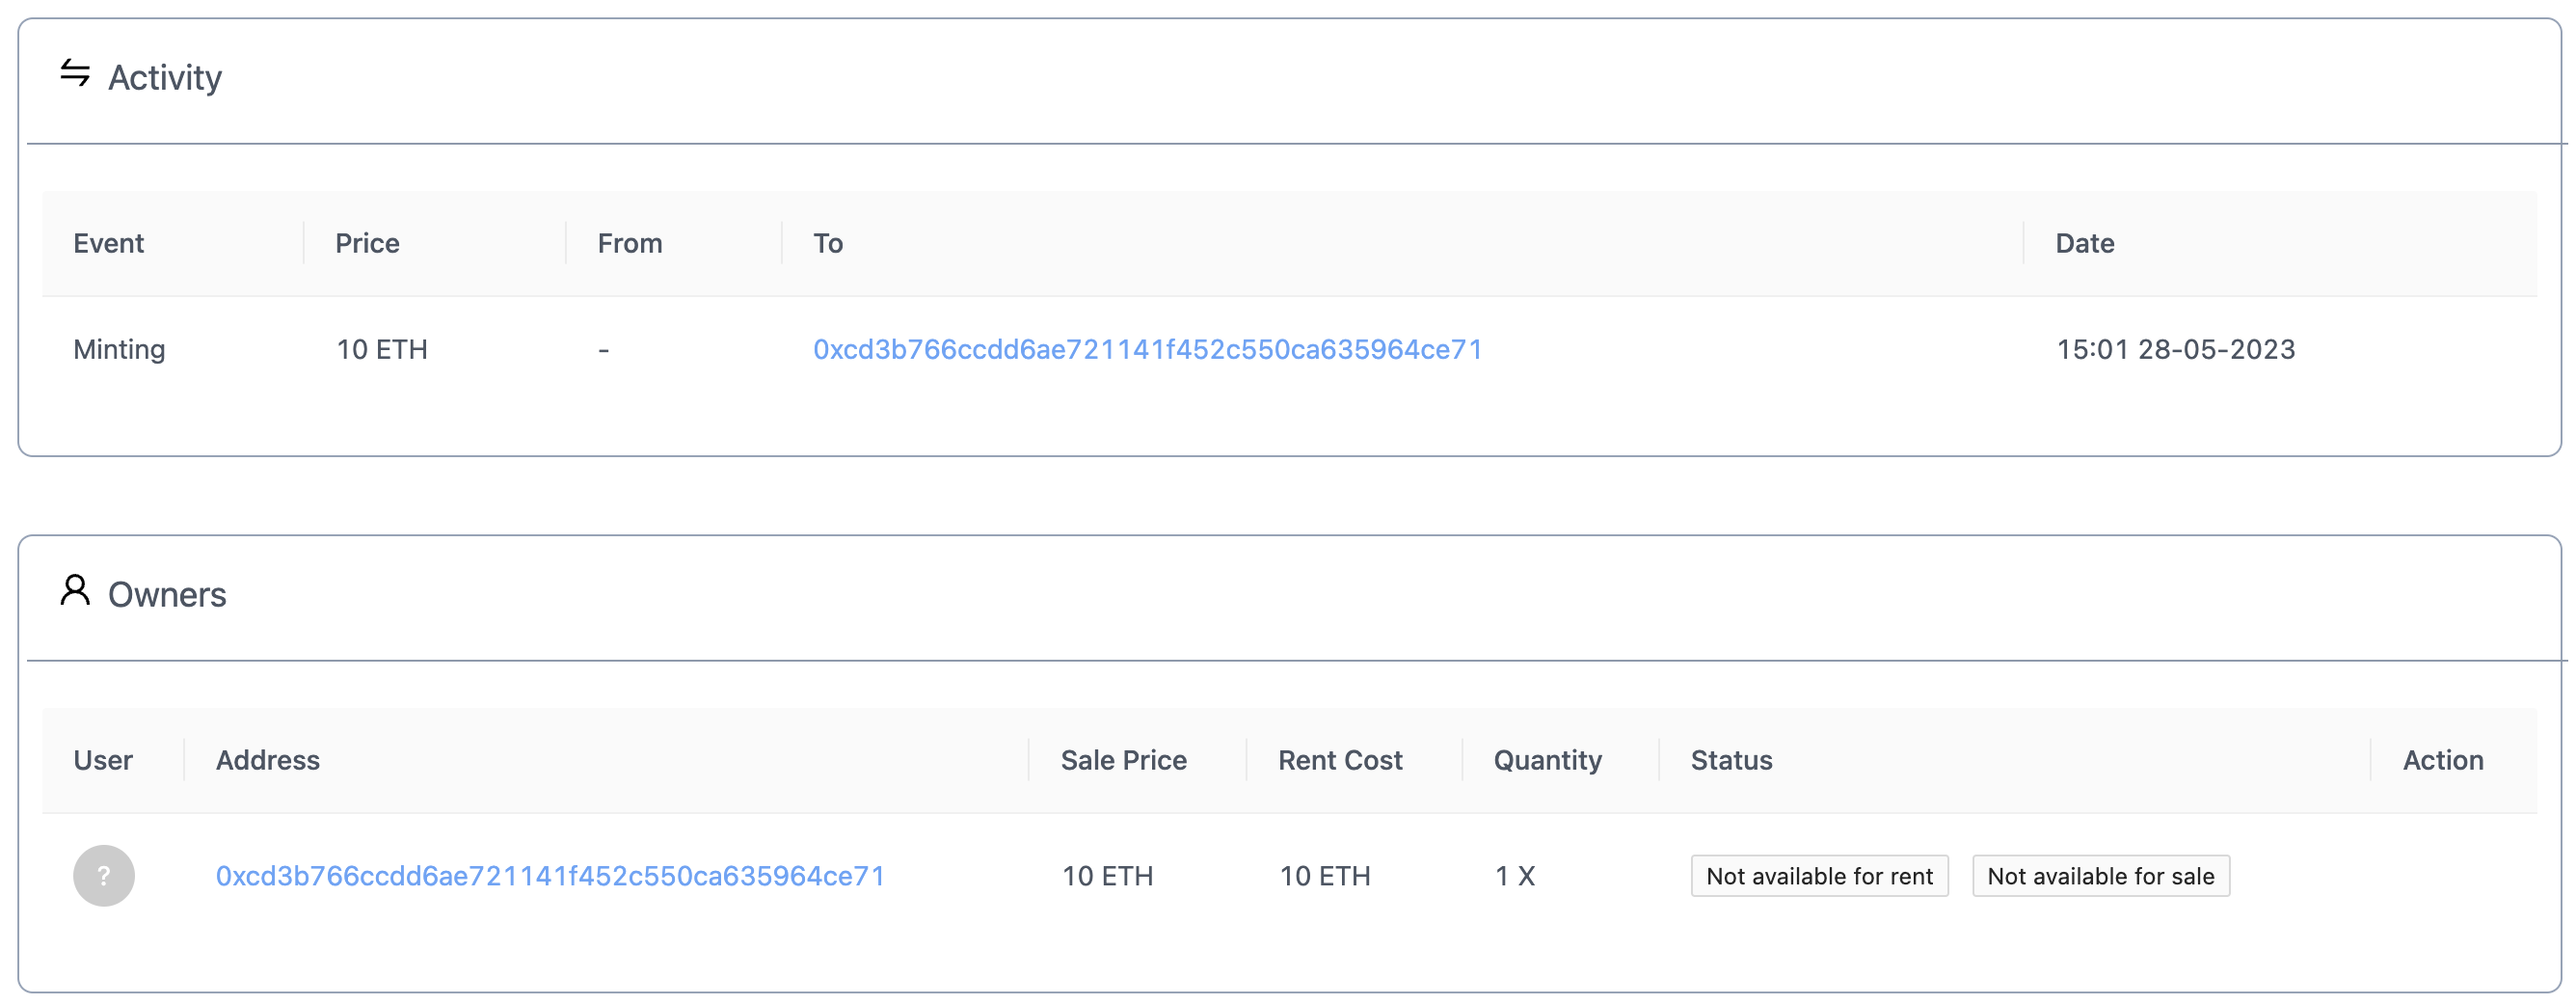
\includegraphics[scale=0.3]{gambar/img-test-rent-mint-3.png}
          \caption{Hasil minting token-2}
          \label{fig:TestRentHasilMinting2}
        \end{figure}
        \begin{figure} [H] \centering
          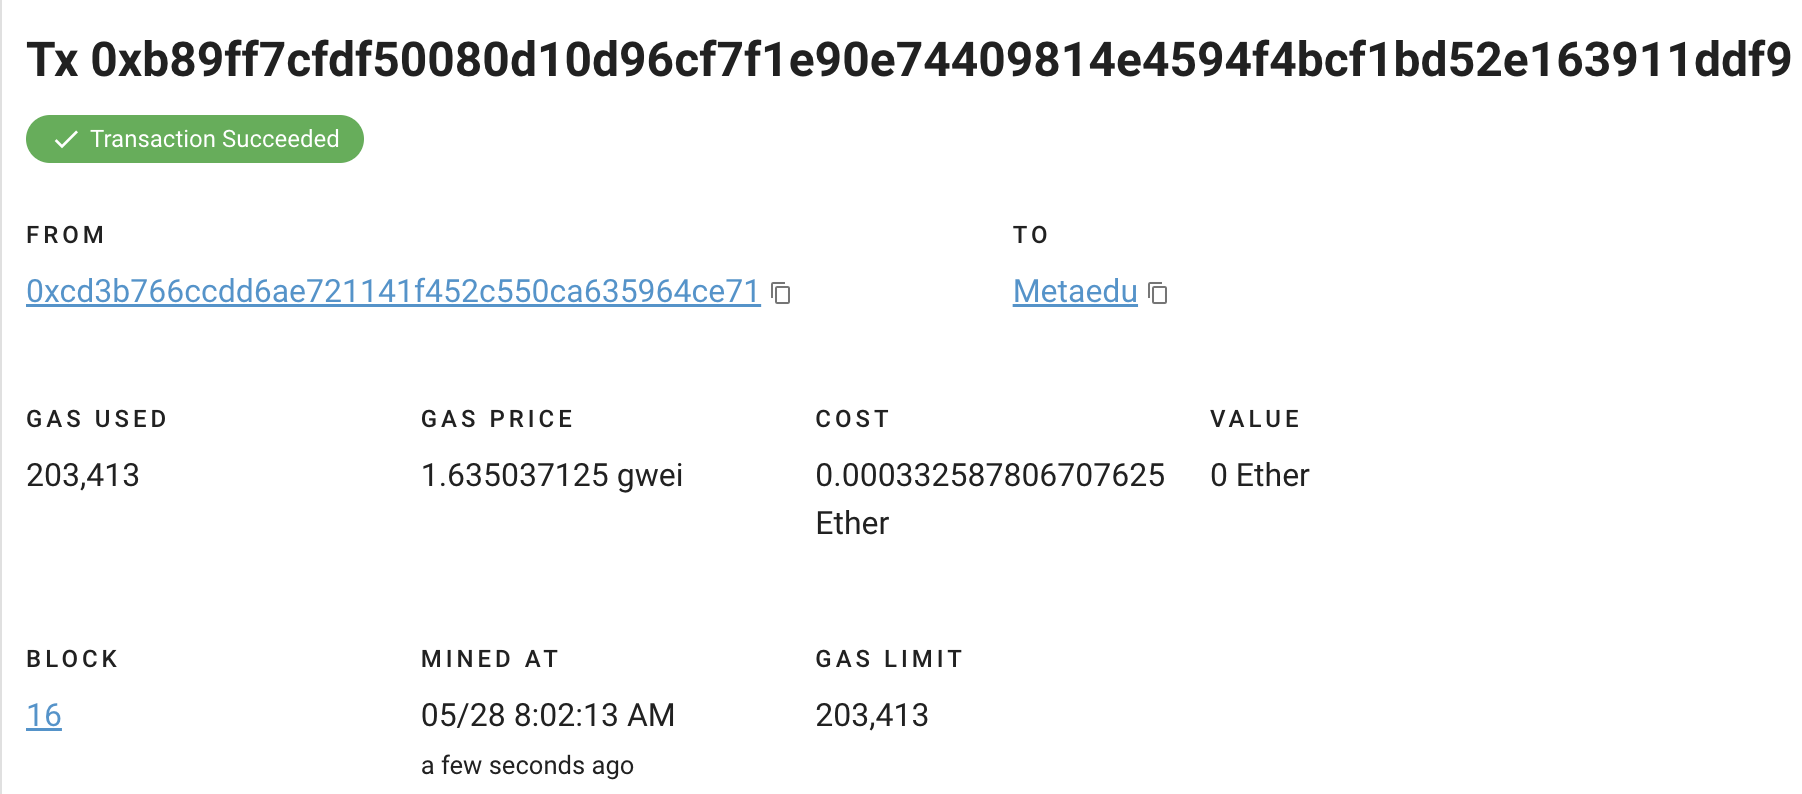
\includegraphics[scale=0.4]{gambar/img-test-rent-mint-4.png}
          \caption{Hasil minting token pada \emph{Ethernal}}
          \label{fig:TestRentHasilMinting3}
        \end{figure}
      Pada gambar dapat diketahui bahwa \emph{gas} yang diperlukan/\emph{gas used} adalah \textbf{220,513} dan \emph{gas price} adalah \textbf{2,006169455} \emph{gwei} maka \emph{gas fee} yang dibayarkan adalah \textbf{0,000442386445030415} \emph{ETH}
      \item Akun A memperbarui status token yang telah di-\emph{minting} supaya dapat disewakan.
      \begin{figure} [H] \centering
          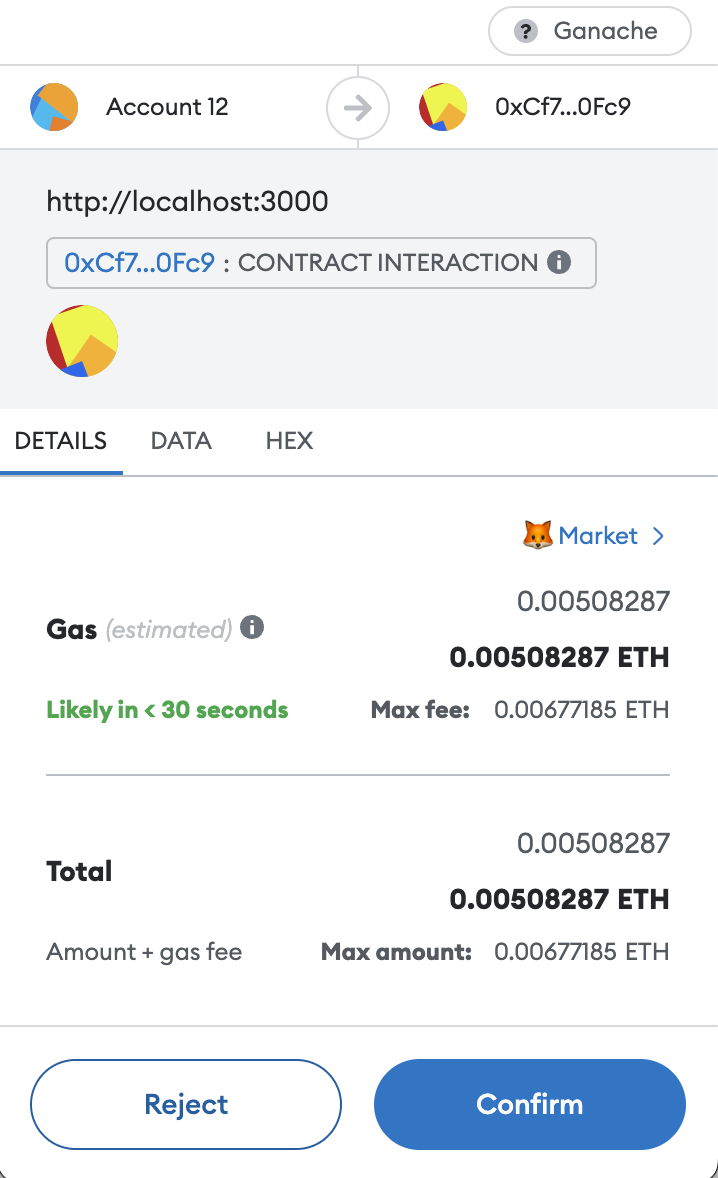
\includegraphics[scale=0.3]{gambar/img-test-rent-put-item-for-rent-1.png}
          \caption{Konfirmasi pembaruan status penyewaan token}
          \label{fig:TestRentKonfirmasiPembaruanPenyewa}
        \end{figure}
        Pada gambar dapat diketahu bahwa estimasi \emph{gas fee} adalah \textbf{0,00508287 \emph{ETH}}.
        \begin{figure} [H] \centering
          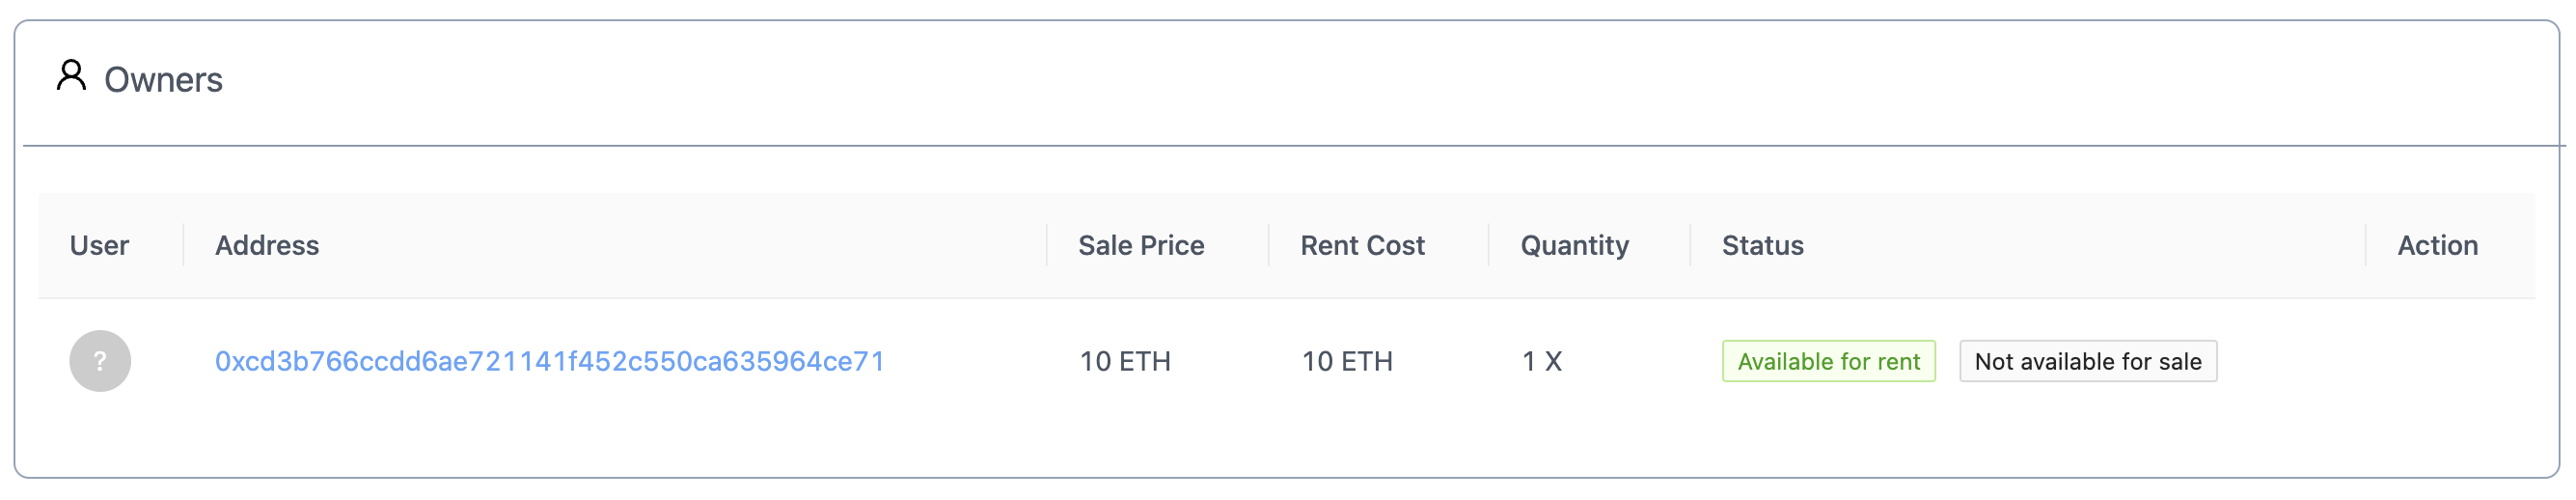
\includegraphics[scale=0.3]{gambar/img-test-rent-put-item-for-rent-2.png}
          \caption{Hasil pembaruan status penyewaan \emph{token}}
          \label{fig:TestRentPutItemForRent}
        \end{figure}
        \begin{figure} [H] \centering
            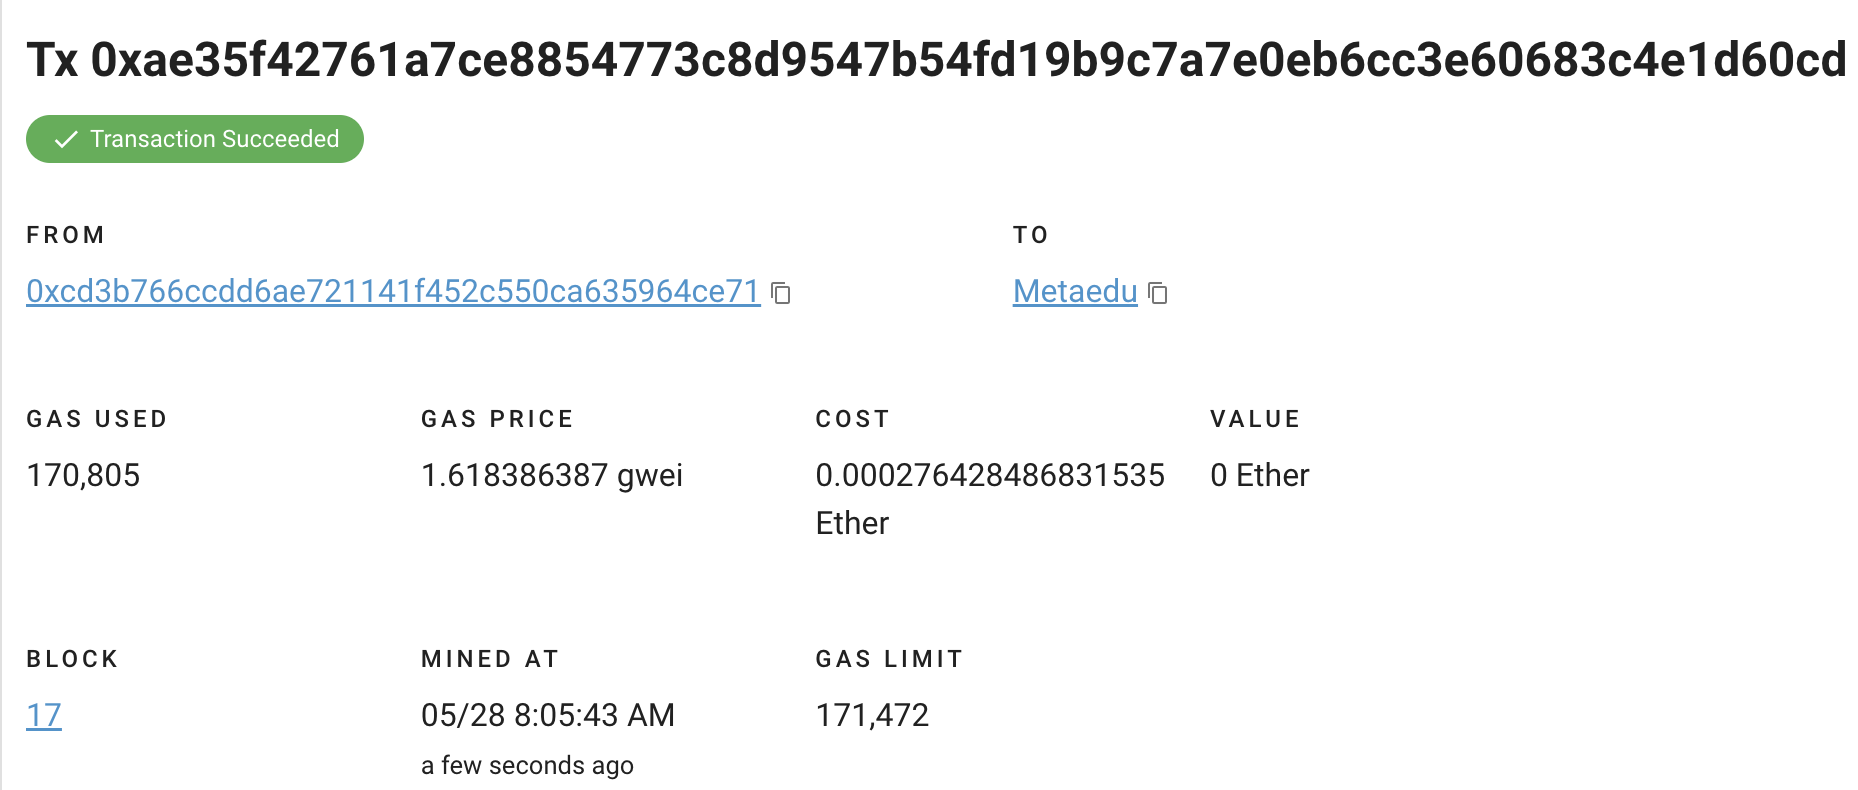
\includegraphics[scale=0.3]{gambar/img-test-rent-put-item-for-rent-3.png}
            \caption{Hasil pembaruan status penyewaan \emph{token} pada \emph{Ethernal}}
            \label{fig:TestRentPutItemForRent2}
          \end{figure}
        Pada gambar dapat diketahui bahwa \emph{gas} yang diperlukan/\emph{gas used} adalah \textbf{170,805} dan \emph{gas price} adalah \textbf{1,618386387 \emph{gwei}} maka \emph{gas fee} yang dibayarkan adalah \textbf{0,000276428486831535 \emph{ETH}}.
      \item Akun A memperbarui harga sewa \emph{token} menjadi \textbf{1 \emph{ETH}} per hari
      \begin{figure} [H] \centering
        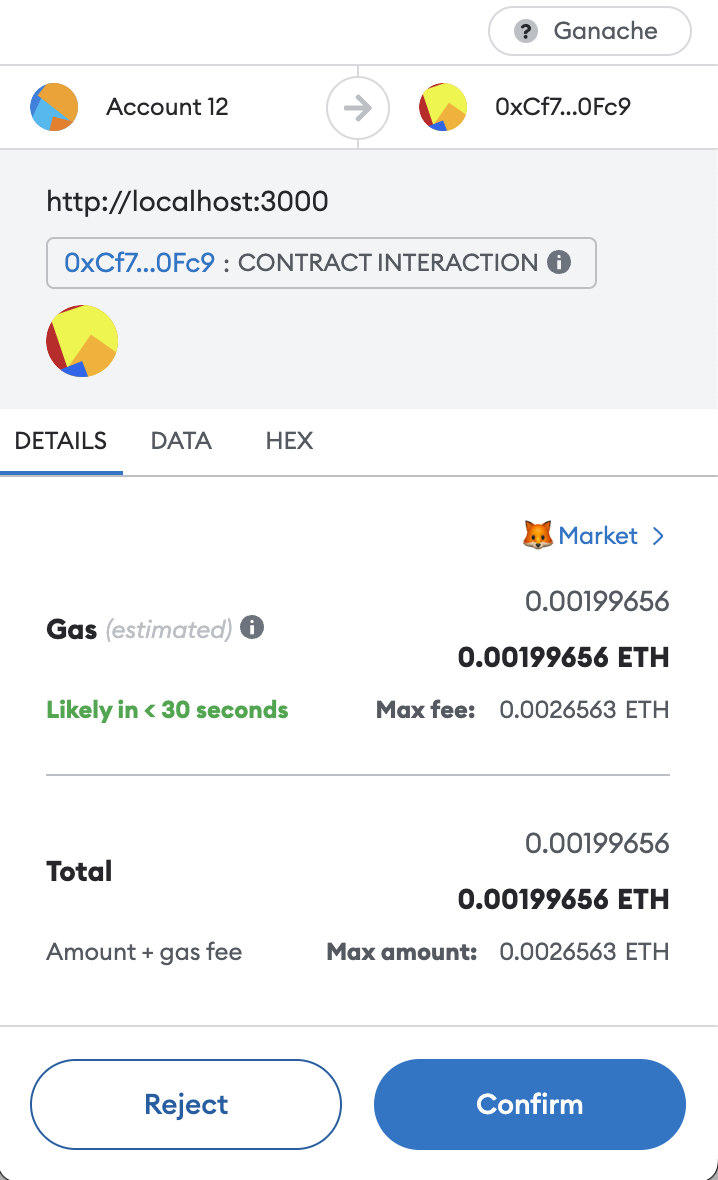
\includegraphics[scale=0.3]{gambar/img-test-rent-put-item-for-rent-2-1.png}
        \caption{Konfirmasi pembaruan harga sewa token}
        \label{fig:TestRentKonfirmasiPembaruanPenyewa2-1}
      \end{figure}
      Pada gambar dapat diketahu bahwa estimasi \emph{gas fee} adalah \textbf{0,00199656 \emph{ETH}}.
      \begin{figure} [H] \centering
        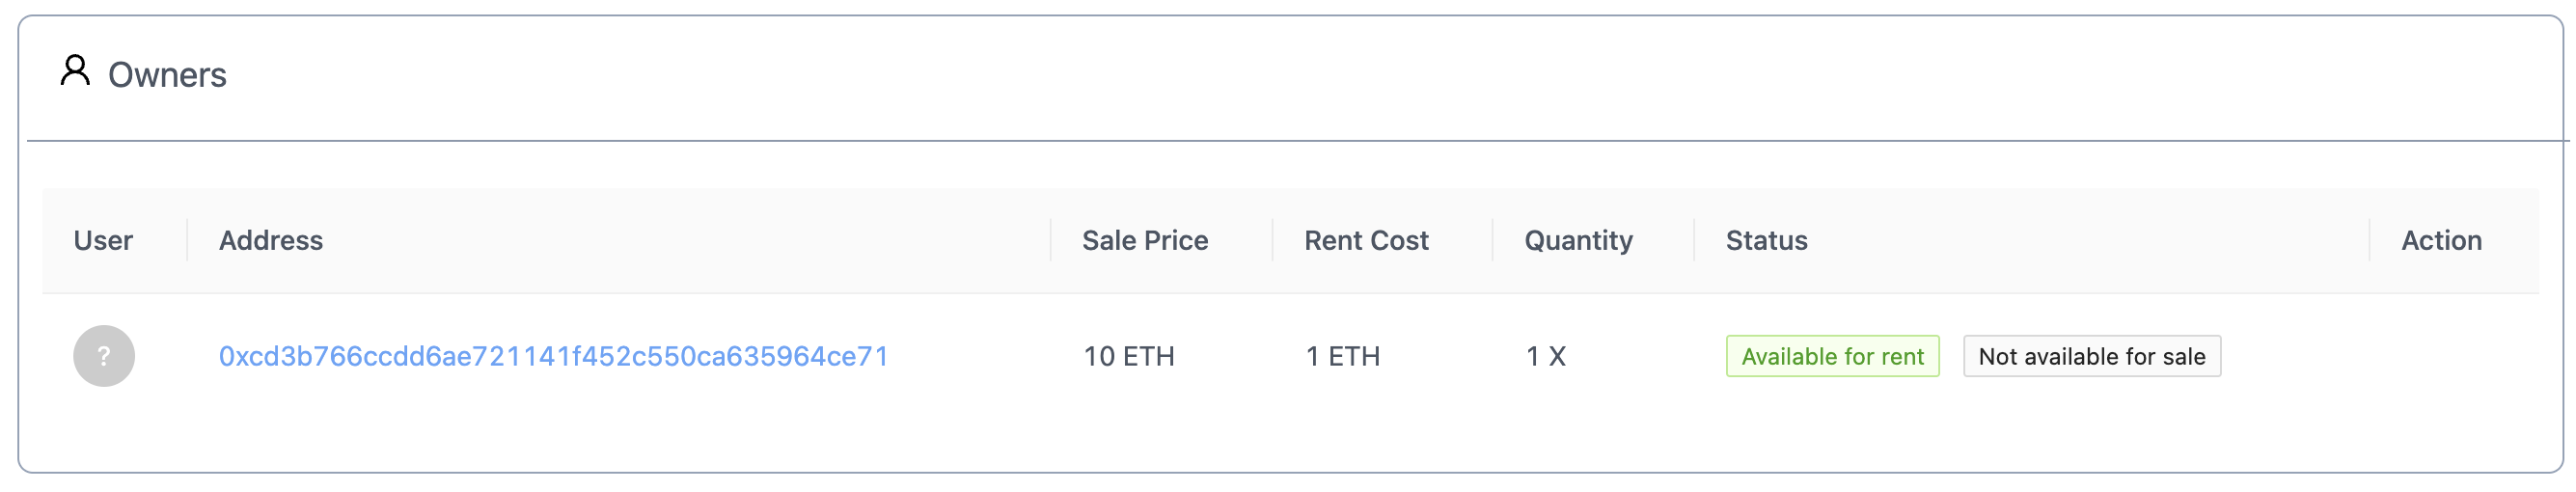
\includegraphics[scale=0.3]{gambar/img-test-rent-put-item-for-rent-2-2.png}
        \caption{Hasil pembaruan harga penyewaan \emph{token}}
        \label{fig:TestRentPutItemForRent2-2}
      \end{figure}
      \begin{figure} [H] \centering
          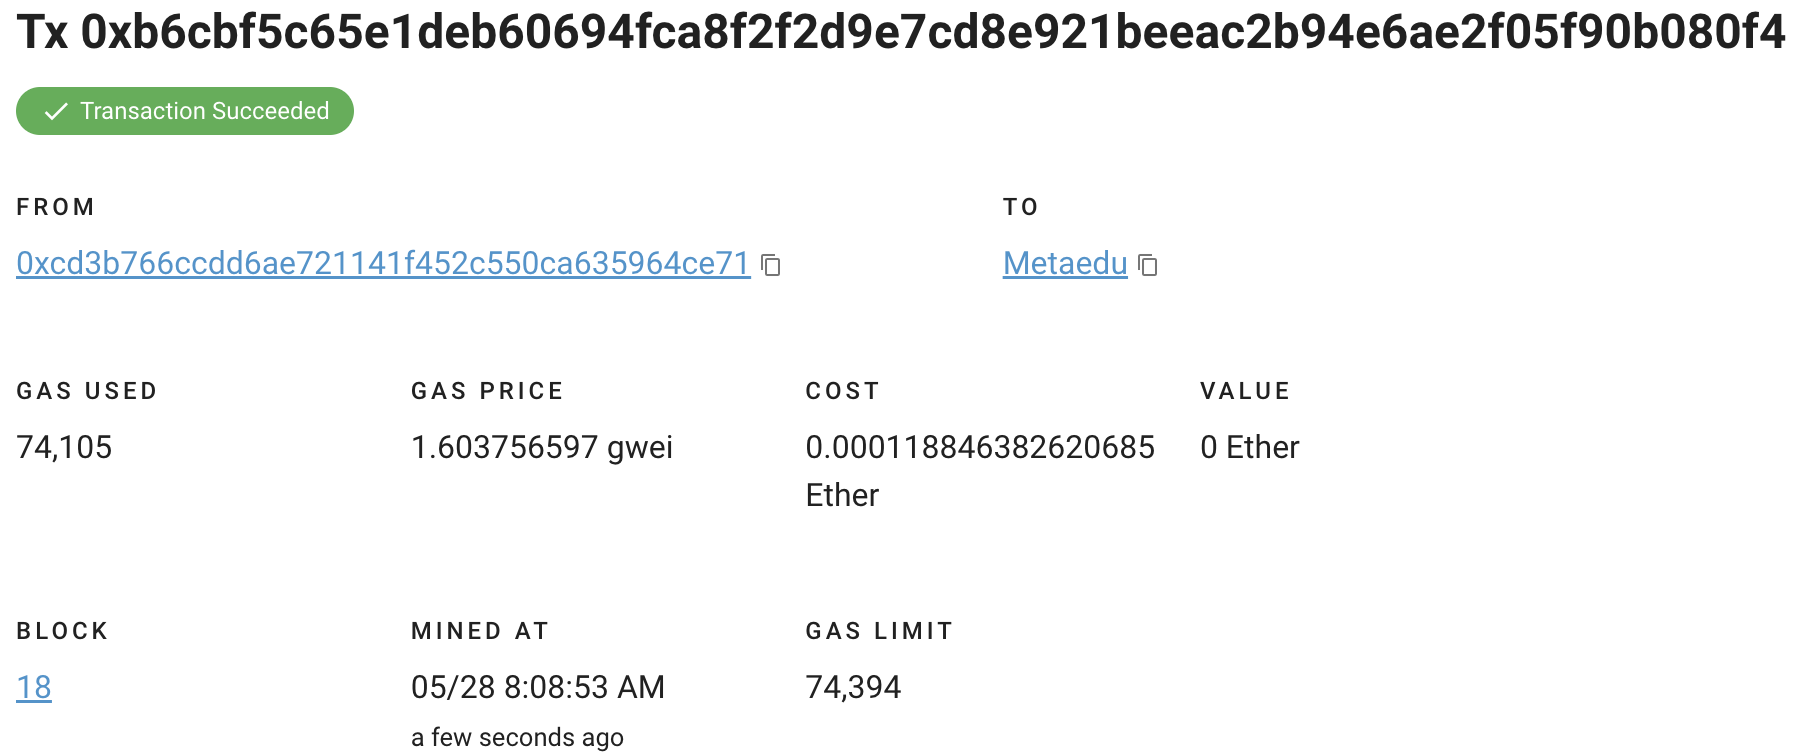
\includegraphics[scale=0.3]{gambar/img-test-rent-put-item-for-rent-2-3.png}
          \caption{Hasil pembaruan status penyewaan \emph{token} pada \emph{Ethernal}}
          \label{fig:TestRentPutItemForRent2-3}
        \end{figure}
      Pada gambar dapat diketahui bahwa \emph{gas} yang diperlukan/\emph{gas used} adalah \textbf{74,105} dan \emph{gas price} adalah \textbf{1,603756597 \emph{gwei}} maka \emph{gas fee} yang dibayarkan adalah \textbf{0,000118846382620685 \emph{ETH}}.
      \item Akun B menyewa \emph{token} yang dimiliki oleh akun A selama 3 hari
        \begin{figure} [H] \centering
            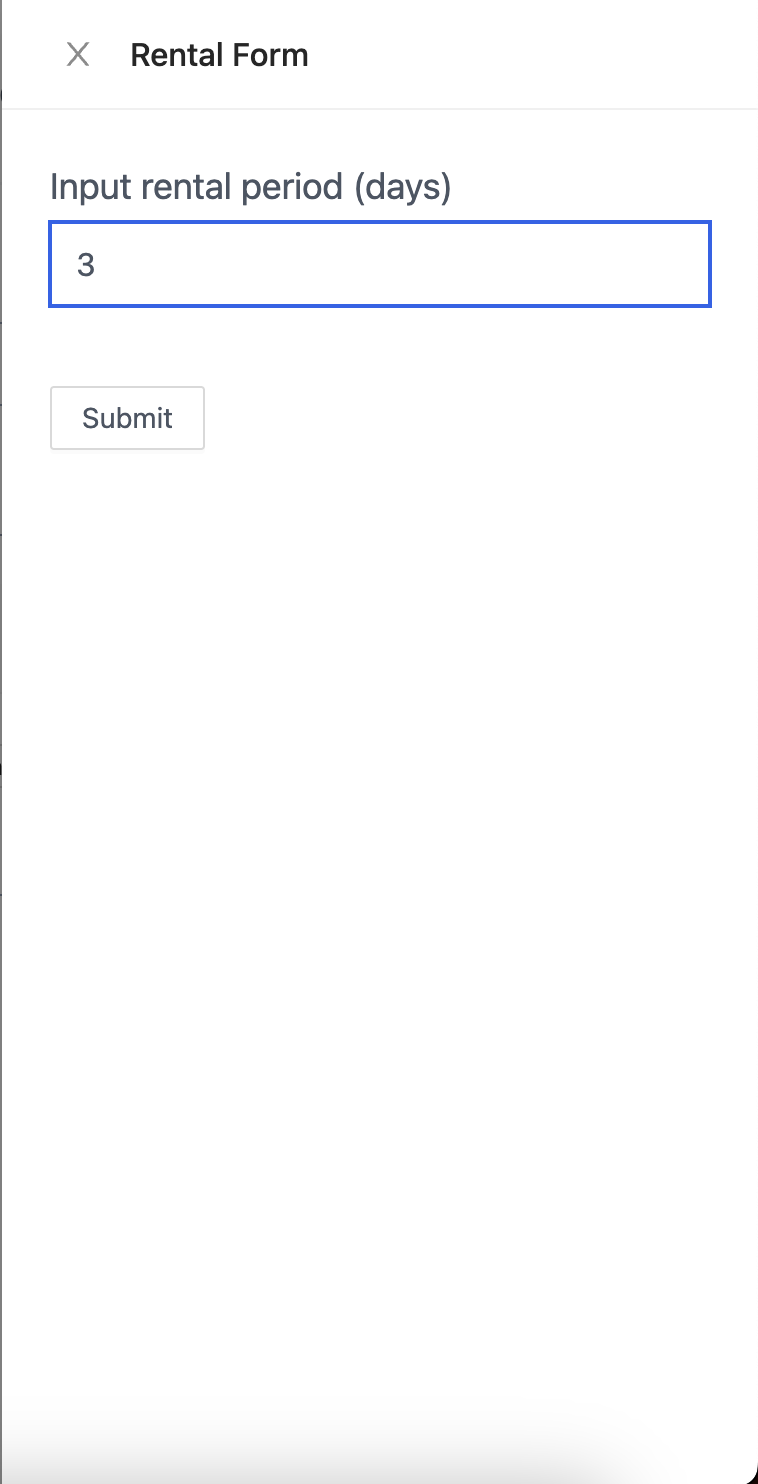
\includegraphics[scale=0.4]{gambar/img-test-rent-rent-1.png}
            \caption{Input lama penyewaan \emph{token}}
            \label{fig:TestRentInputRentalPeriodToken}
          \end{figure}

          \begin{figure} [H] \centering
        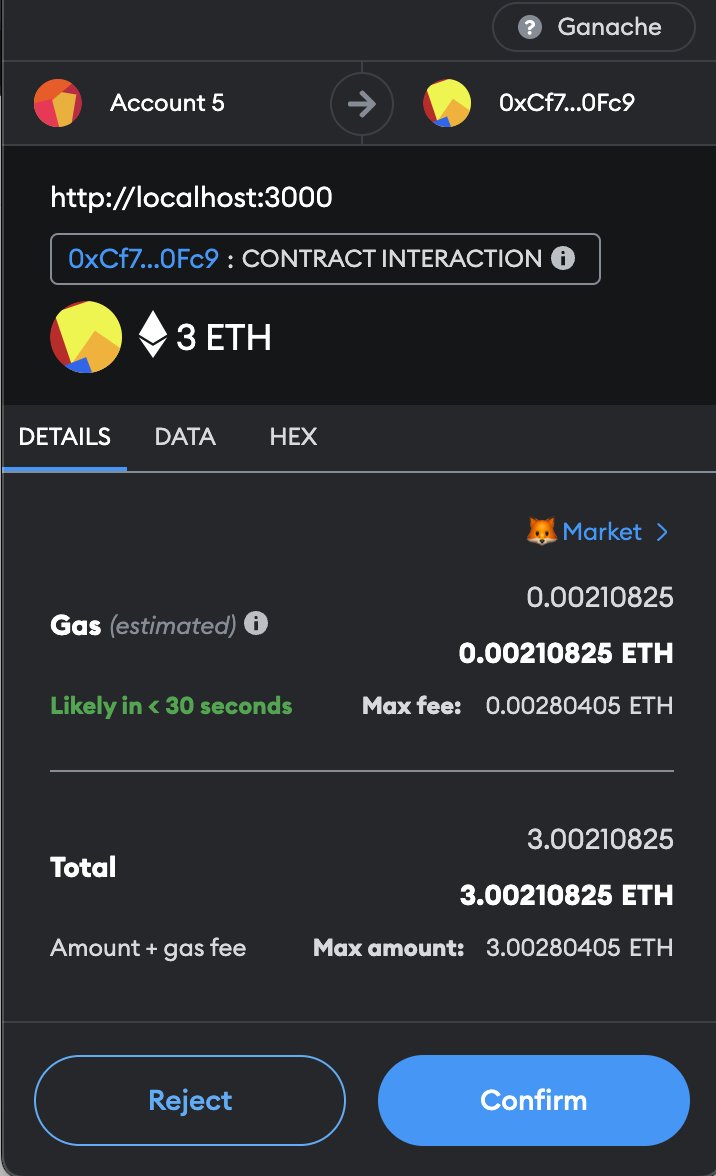
\includegraphics[scale=0.4]{gambar/img-test-rent-rent-2.png}
        \caption{Konfirmasi penyewaan \emph{token}}
        \label{fig:TestRentKonfirmasiPenyewaanToken}
      \end{figure}
        Pada gambar dapat diketahui bahwa estimasi \emph{gas} adalah \textbf{0,00210825 \emph{ETH}} dan biaya penyewaan adalah \textbf{3 ETH} sesuai dengan harga sewa \emph{token} dan lama penyewaan
      \begin{figure} [H] \centering
          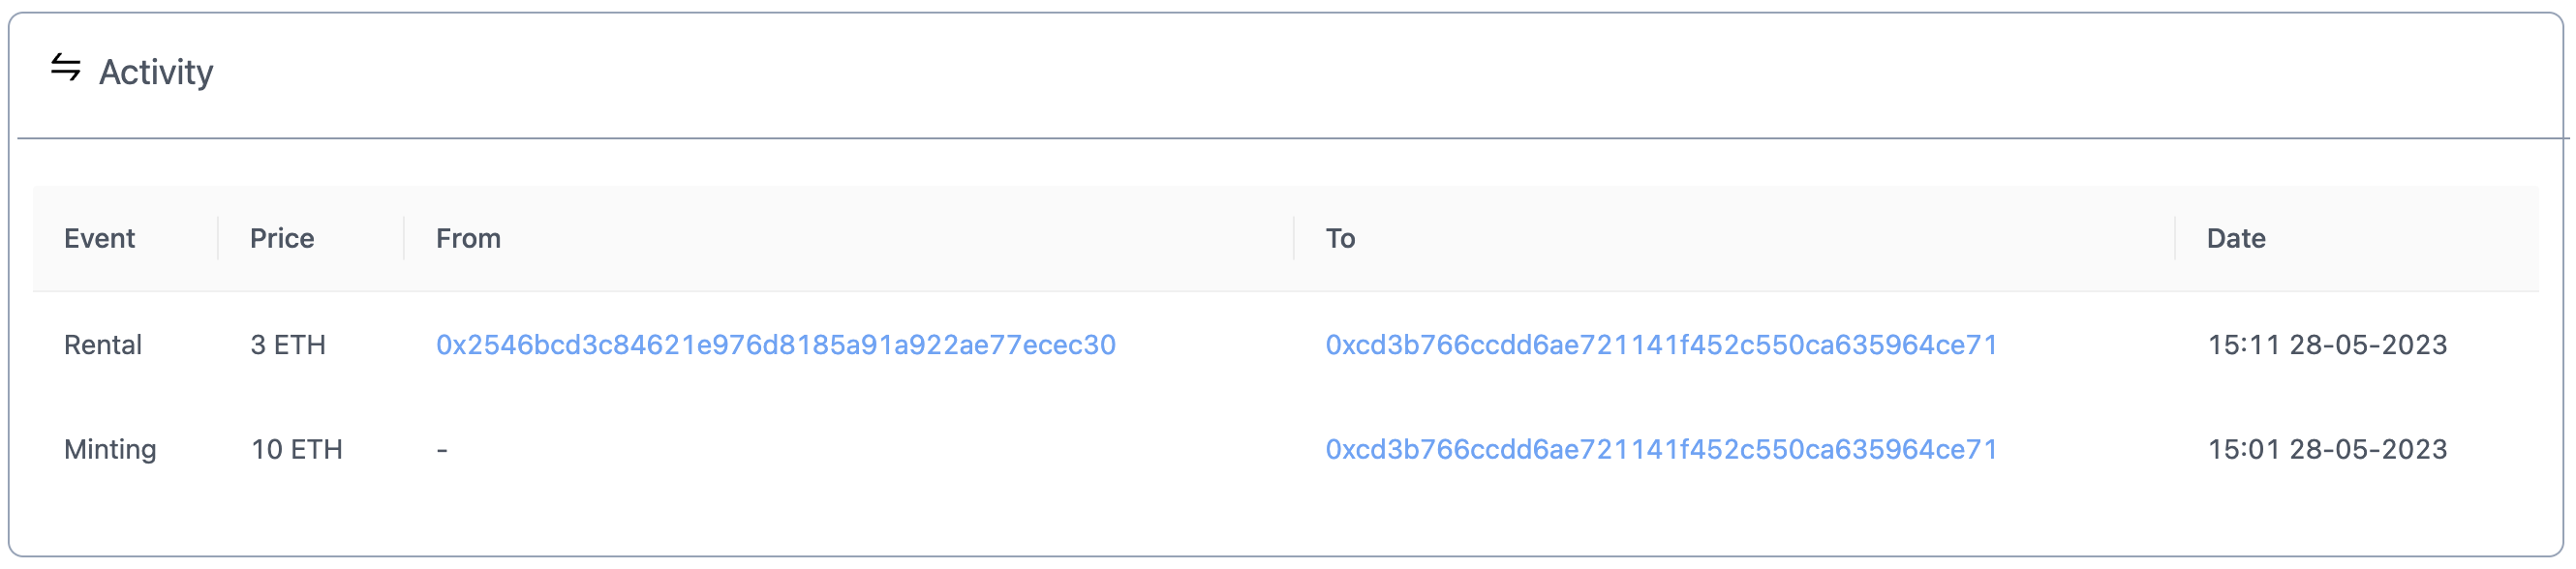
\includegraphics[scale=0.3]{gambar/img-test-rent-rent-3.png}
          \caption{Hasil penyewaan token}
          \label{fig:TestRentResultRental}
        \end{figure}
        Setelah dilakukan penyewaan maka data penyewaan akan tecatat pada tabel \emph{activity}.
        \begin{figure} [H] \centering
          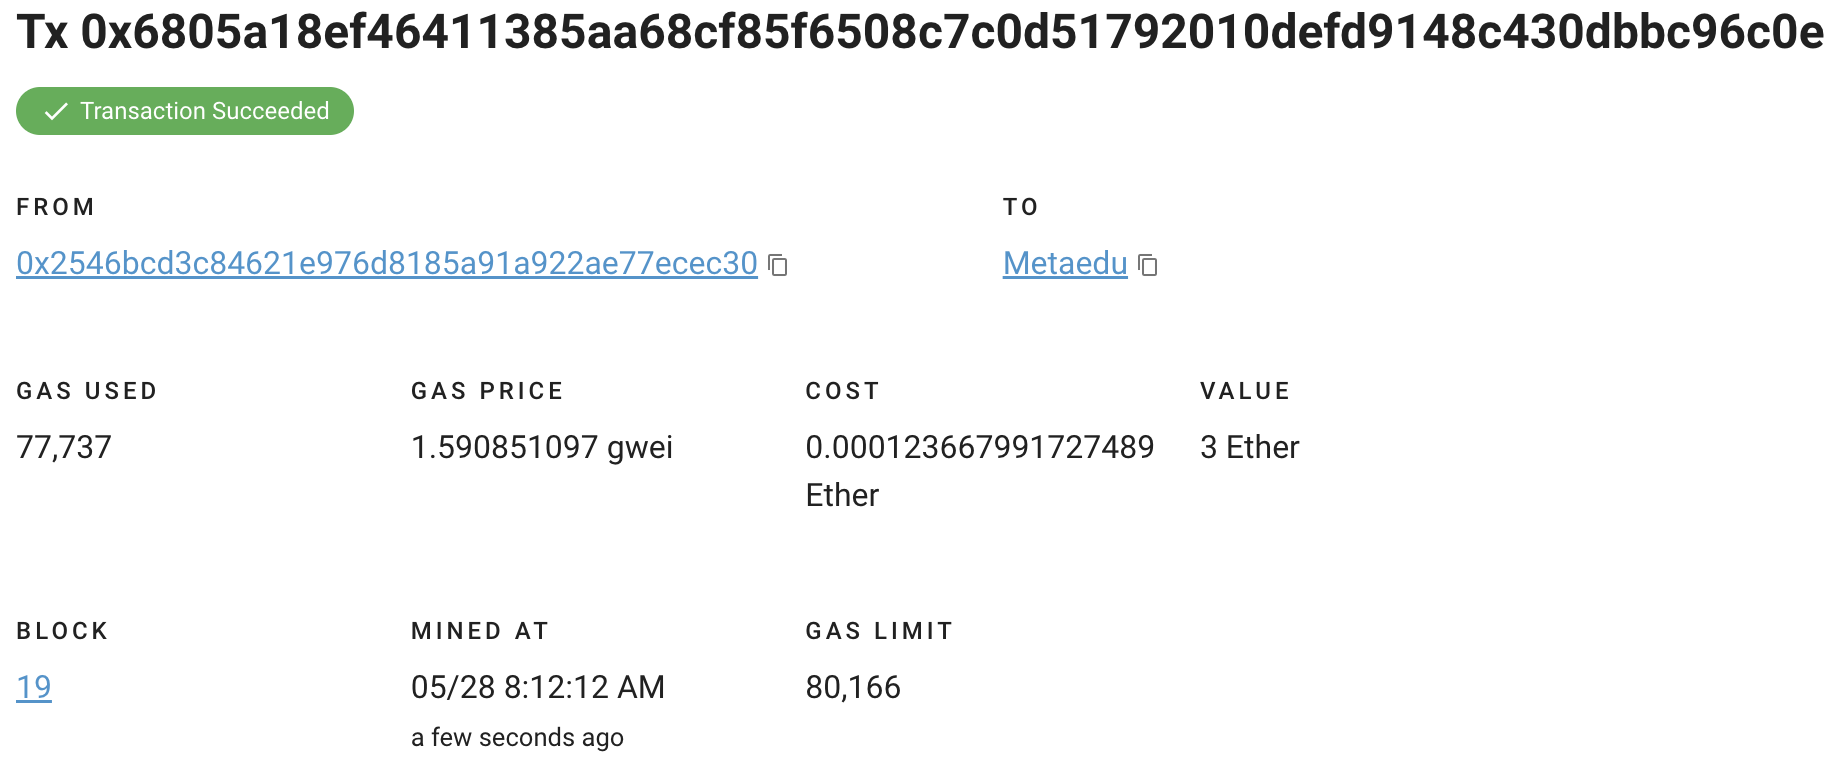
\includegraphics[scale=0.4]{gambar/img-test-rent-rent-4.png}
          \caption{Hasil penyewaan token pada \emph{Ethernal}}
          \label{fig:TestRentResultRental2}
        \end{figure}
        Pada gambar dapat diketahui bahwa \emph{gas} yang diperlukan/\emph{gas used} adalah \textbf{77,737} dan \emph{gas price} adalah \textbf{1,590851097 \emph{gwei}} maka \emph{gas fee} yang dibayarkan adalah \textbf{0.000123667991727489 \emph{ETH}}.
      Saldo dari \emph{wallet} akun B berkurang sebesar \textbf{3 \emph{ETH}} ditambah dengan \emph{gas fee} yang diperlukan pada transaksi sebelumnya menjadi 9989.9998 \emph{ETH}.
      \begin{figure} [H] \centering
          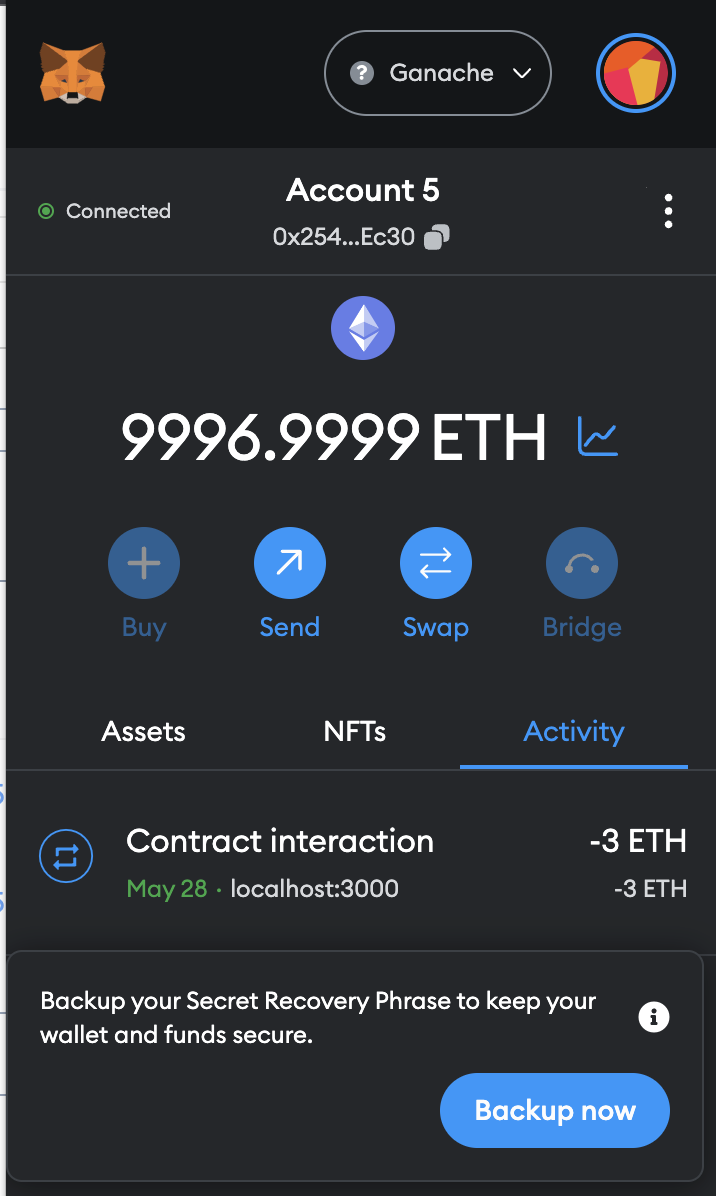
\includegraphics[scale=0.4]{gambar/img-test-rent-rent-5.png}
          \caption{Saldo akun B setelah menyewa \emph{token}}
          \label{fig:TestRentResultRental3}
        \end{figure}
      Saldo dari \emph{wallet} akun A bertambah sebesar \textbf{3 \emph{ETH}} dikurangi dengan \emph{gas fee} yang diperlukan pada transaksi sebelumnya menjadi 9989.9998 \emph{ETH}. 
      \begin{figure} [H] \centering
        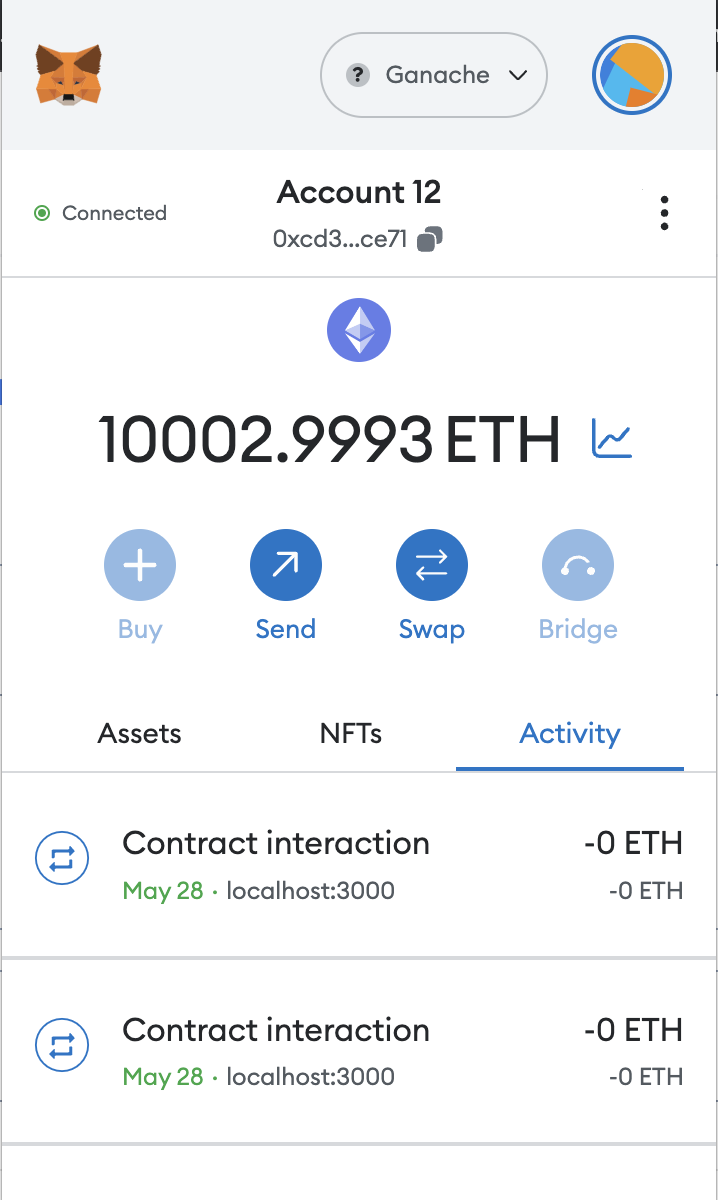
\includegraphics[scale=0.4]{gambar/img-test-rent-rent-6.png}
        \caption{Saldo akun A bertambah setelah token yang dimiliki disewa}
        \label{fig:TestRentResultRental4}
      \end{figure}
    \end{itemize}
  
  Setelah dilakukan pengujian penyewaan maka dapat disimpulkan bahwa alur dari aplikasi telah berjalan sesuai dengan harapan pengujian yang telah disebutkan di awal. Selain itu juga diperoleh data mengenai \emph{gas fee} sesuai dengan tabel berikut
  
  \begin{longtable}{|c|c|c|c|}
      \caption{\emph{Gas fee} yang diperoleh selama pengujian \emph{flow} penyewaan}
      \label{tb:EnergiKecepatan}                                   \\
      \hline
      \rowcolor[HTML]{C0C0C0}
      \textbf{\emph{Function}} & \textbf{\emph{Gas used}} & \textbf{\emph{Gas price}} & \textbf{\emph{Gas fee} yang dibayarkan (\emph{ETH})} \\
      \hline
      \emph{mint}  & 203,413 & 1,635037125    & 0,000442386445030415    \\
      \emph{putItemForRent (1)}  & 170,805 & 1,6183836    & 0,000276428486831535    \\
      \emph{putItemForRent (2)} & 74,105 & 1,603756    & 0,000118846382620685      \\
      \emph{rent}               & 77,737 & 1,590851097    & 0.000123667991727489      \\
      \hline
    \end{longtable}

\subsection{\emph{Flow} Pembagian Kepemilikan}

Pada pengujian \emph{flow} pembegaian kepemilikan hal-hal yang diharapkan antara lain adalah:
\begin{itemize}
    \item Pemilik \emph{token} dapat membagi kepemilikan \emph{token} yang dimiliki dengan pengguna lain.
    \item \emph{Token} yang dibagi kepemilikannya akan membuat token asalnya menjadi dimiliki oleh pemilik kontrak dan melakukan \emph{minting} \emph{fraction} \emph{token}  dengan suplai yang merepresentasikan jumlah kepemilikan atas token asal. 
    \item \emph{Token} asal dapat disewakan dan keuntungan dari hasil sewa akan dibagian ke pengguna pemilik \emph{fraction} \emph{token}.
    \item Saldo \emph{wallet} pemilik \emph{fraction token} bertambah sesuai dengan harga dan jumlah kepemilikannya atas \emph{fraction token} dibanding suplai yang beredar.
    \item Saldo \emph{wallet} penyewa berkurang sesuai dengan harga dan lama sewa.
    \item Seluruh data terkait dengan kepemilikan, penjualan, dan penyewaan dari \emph{token} di halaman web sesuai dengan alur pengujian  
\end{itemize}

Berikut merupakan data mengenai \emph{wallet} yang digunakan dalam pengujian:

% Contoh pembuatan tabel
\begin{longtable}{|c|c|c|}
    \caption{Kondisi awal}
    \label{tb:EnergiKecepatan}                                   \\
    \hline
    \rowcolor[HTML]{C0C0C0}
    \textbf{\emph{Akun}} & \textbf{\emph{Address}} & \textbf{Saldo (\emph{ETH})}\\
    \hline
    A & 0xbDA5747bFD65F08deb54cb465eB87D40e51B197E            & 10000               \\
    B & 0x976EA74026E726554dB657fA54763abd0C3a0aa9            & 10000               \\
    C & 0x9965507D1a55bcC2695C58ba16FB37d819B0A4dc            & 10000               \\
    \hline
  \end{longtable}


  Berikut merupakan langkah-langkah pengujian yang akan dilakukan:
  \begin{itemize}
      \item Akun A melakukan \emph{minting token} dengan suplai 1 token dan harga 10 ETH.
      \begin{figure} [H] \centering
          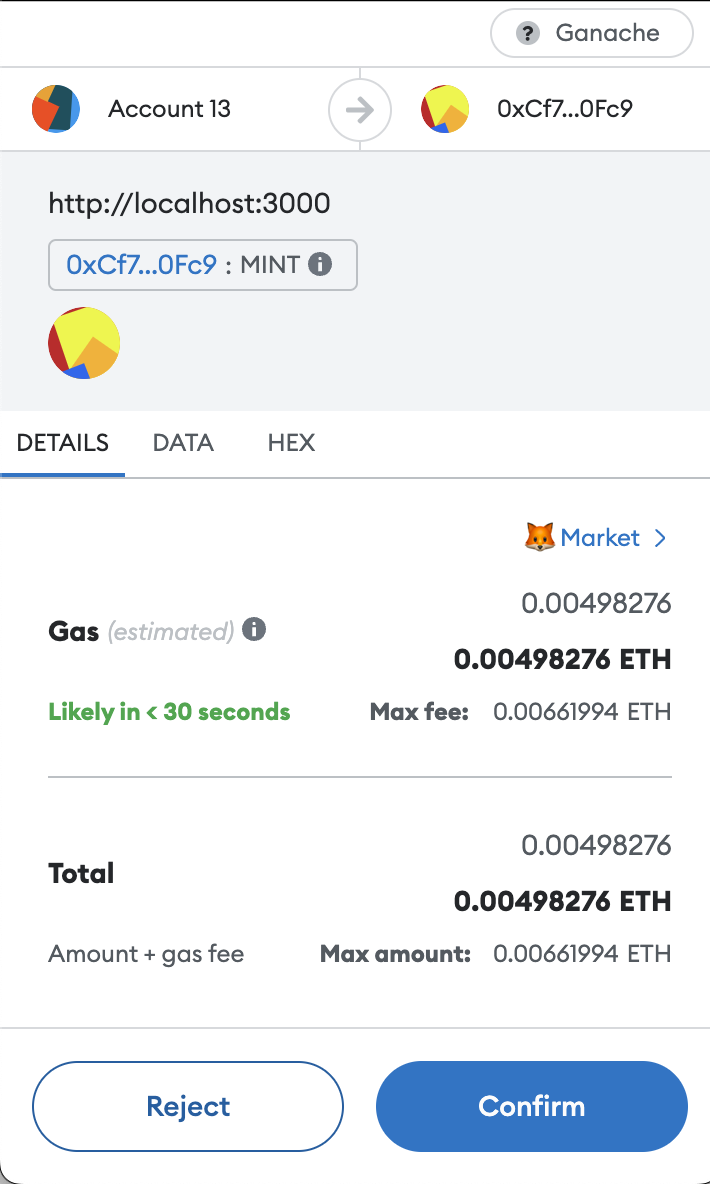
\includegraphics[scale=0.4]{gambar/img-test-share-mint-1.png}
          \caption{Konfirmasi \emph{minting} token}
          \label{fig:TestShareKonfirmasiMintingToken}
        \end{figure}
      Pada gambar terlihat bahwa estimasi \emph{gas} adalah \textbf{0,00498276} \emph{ETH}
      \begin{figure} [H] \centering
          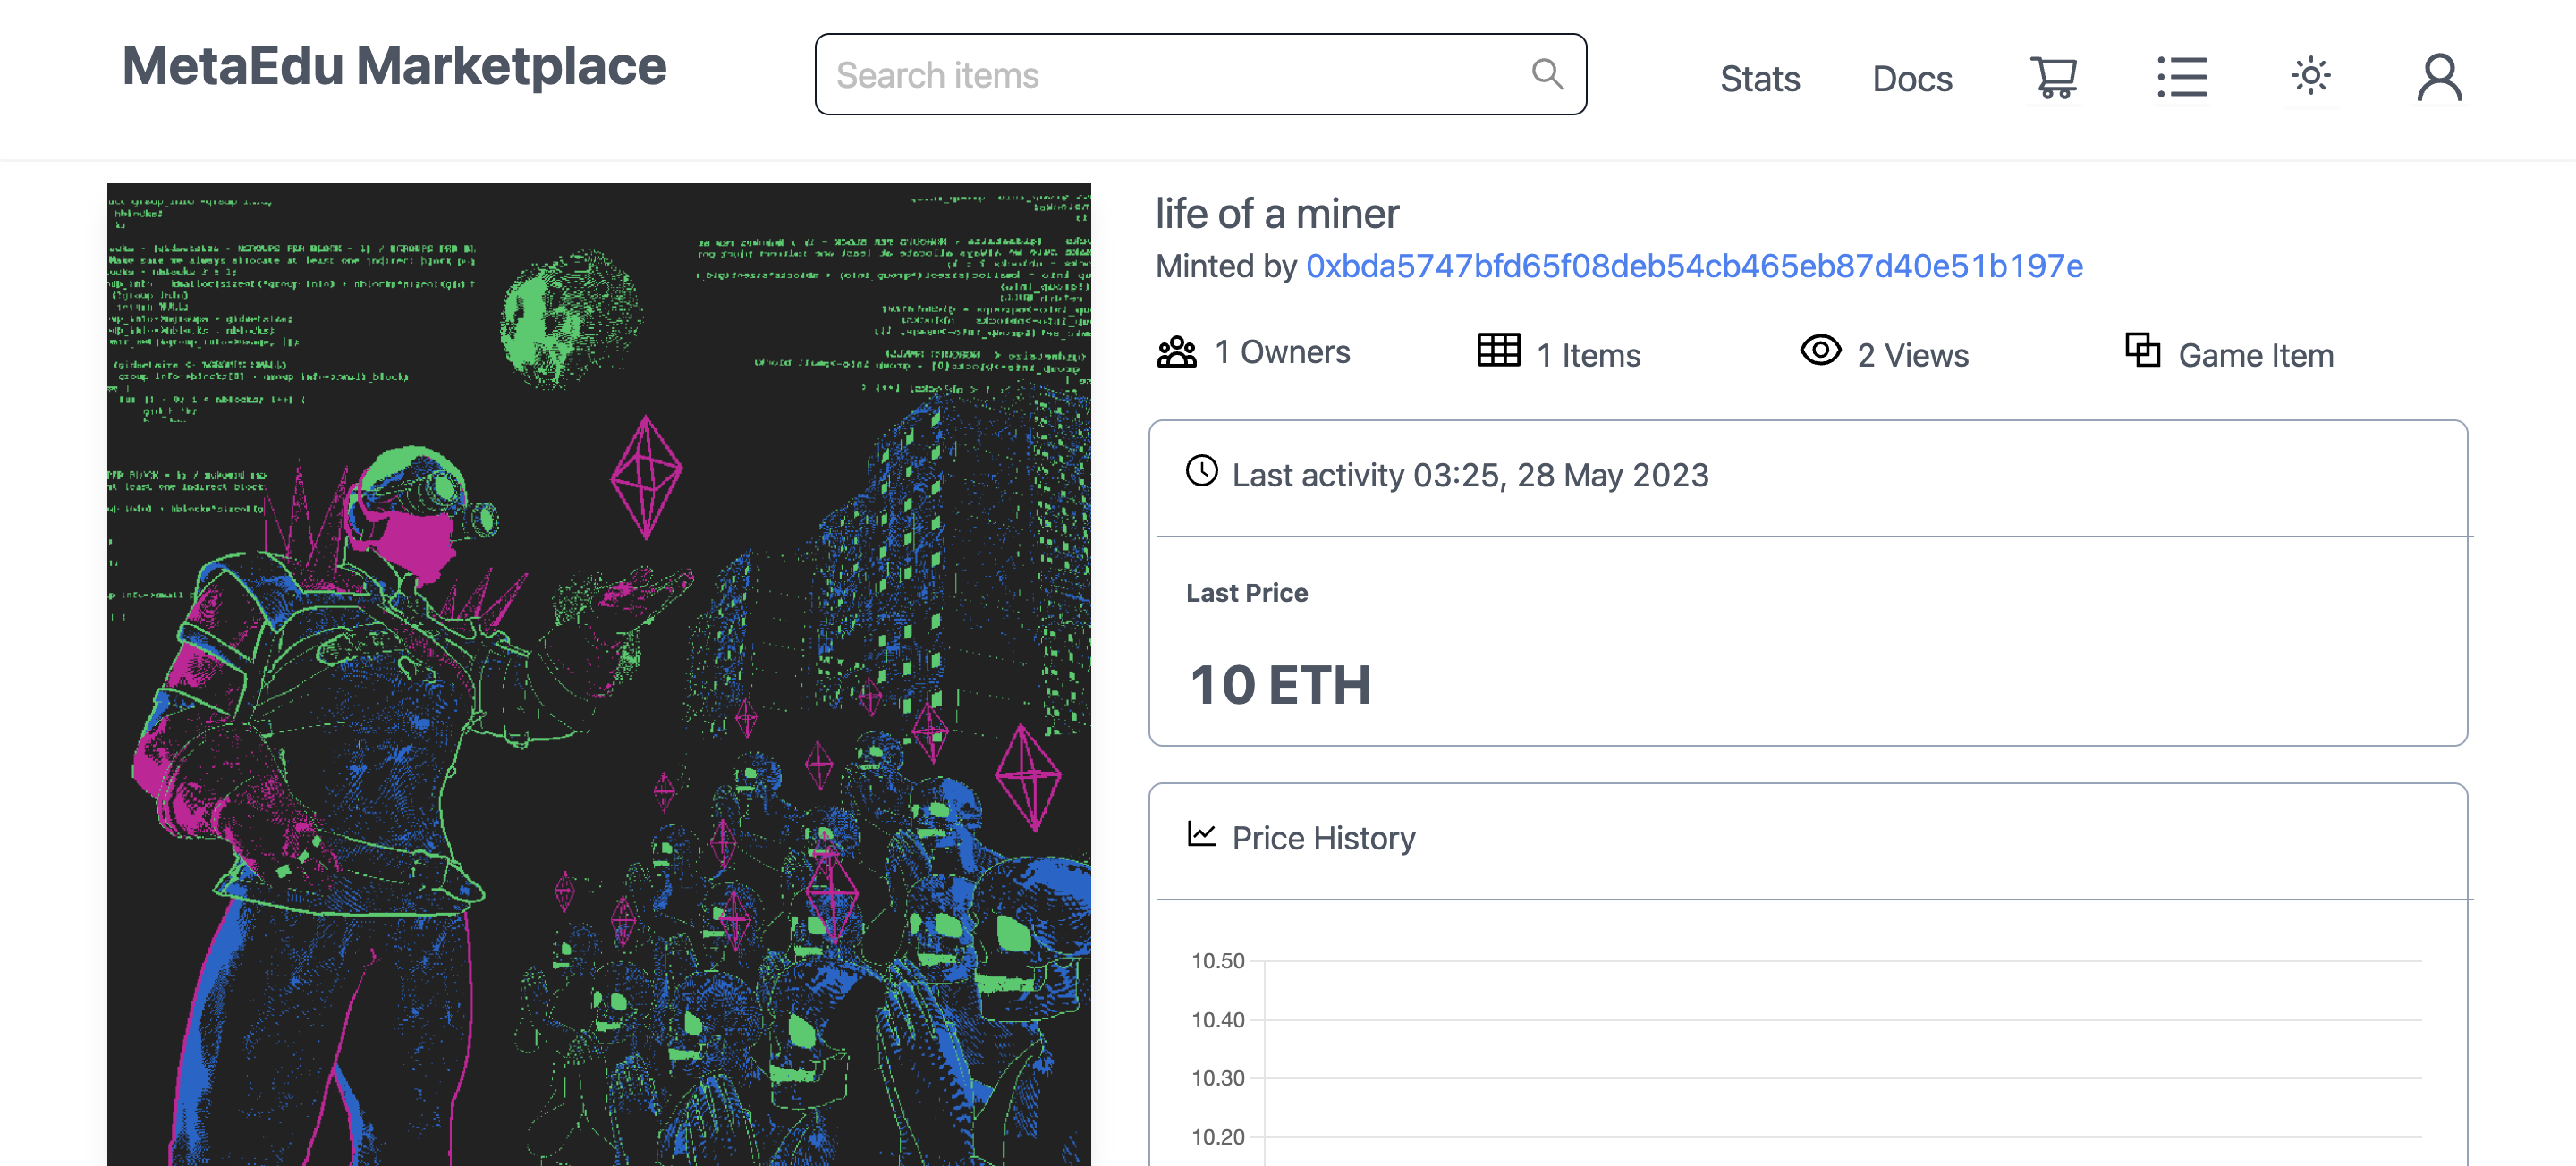
\includegraphics[scale=0.3]{gambar/img-test-share-mint-2.png}
          \caption{Hasil minting token-1}
          \label{fig:TestShareHasilMinting}
        \end{figure}
        \begin{figure} [H] \centering
          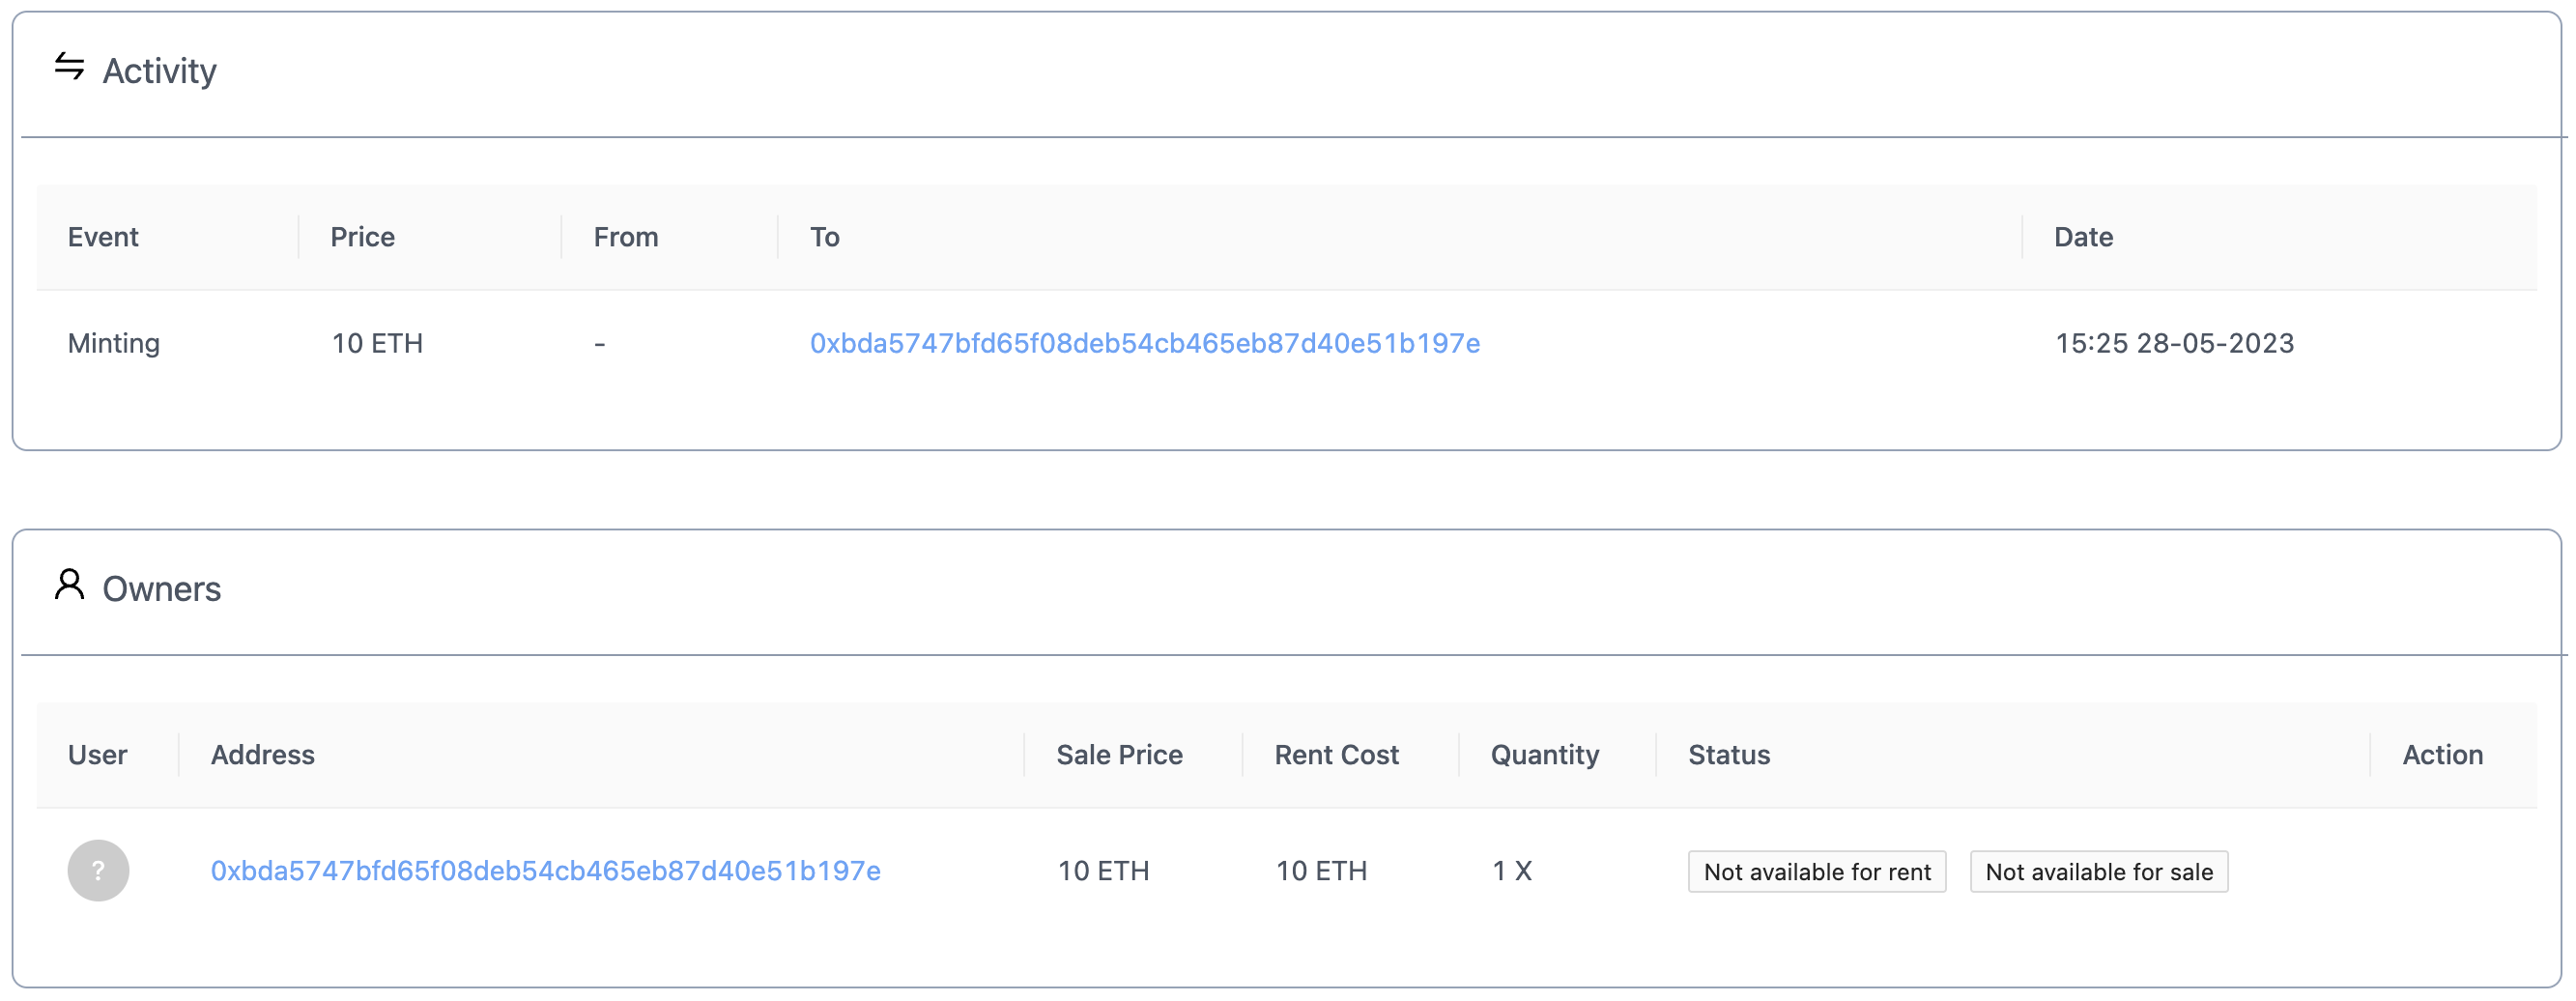
\includegraphics[scale=0.3]{gambar/img-test-share-mint-3.png}
          \caption{Hasil minting token-2}
          \label{fig:TestShareHasilMinting2}
        \end{figure}
        \begin{figure} [H] \centering
          \includegraphics[scale=0.4]{gambar/img-test-share-mint-4.png}
          \caption{Hasil minting token pada \emph{Ethernal}}
          \label{fig:TestShareHasilMinting3}
        \end{figure}
      Pada gambar dapat diketahui bahwa \emph{gas} yang diperlukan/\emph{gas used} adalah \textbf{220,413} dan \emph{gas price} adalah \textbf{1,57955364} \emph{gwei} maka \emph{gas fee} yang dibayarkan adalah \textbf{0,000321301729113932} \emph{ETH}
      \item Akun A memperbarui status token yang telah di-\emph{minting} supaya dapat disewakan.
      \begin{figure} [H] \centering
          \includegraphics[scale=0.3]{gambar/img-test-share-put-item-for-rent-1.png}
          \caption{Konfirmasi pembaruan status penyewaan token}
          \label{fig:TestShareKonfirmasiPembaruanPenyewa}
        \end{figure}
        Pada gambar dapat diketahu bahwa estimasi \emph{gas fee} adalah \textbf{0,00425969 \emph{ETH}}.
        \begin{figure} [H] \centering
          \includegraphics[scale=0.3]{gambar/img-test-share-put-item-for-rent-2.png}
          \caption{Hasil pembaruan status penyewaan \emph{token}}
          \label{fig:TestSharePutItemForRent}
        \end{figure}
        \begin{figure} [H] \centering
            \includegraphics[scale=0.3]{gambar/img-test-share-put-item-for-rent-3.png}
            \caption{Hasil pembaruan status penyewaan \emph{token} pada \emph{Ethernal}}
            \label{fig:TestSharePutItemForRent2}
          \end{figure}
        Pada gambar dapat diketahui bahwa \emph{gas} yang diperlukan/\emph{gas used} adalah \textbf{170,805} dan \emph{gas price} adalah \textbf{1,569744221 \emph{gwei}} maka \emph{gas fee} yang dibayarkan adalah \textbf{0,000268120161667905 \emph{ETH}}.
      \item Akun A memperbarui harga sewa \emph{token} menjadi \textbf{1 \emph{ETH}} per hari
      \begin{figure} [H] \centering
        \includegraphics[scale=0.3]{gambar/img-test-share-put-item-for-rent-2-1.png}
        \caption{Konfirmasi pembaruan harga sewa token}
        % Label referensi dari gambar yang diinputkan
        \label{fig:TestShareKonfirmasiPembaruanPenyewa2-1}
      \end{figure}
      Pada gambar dapat diketahu bahwa estimasi \emph{gas fee} adalah \textbf{0,00166636 \emph{ETH}}.
      \begin{figure} [H] \centering
        % Nama dari file gambar yang diinputkan
        \includegraphics[scale=0.3]{gambar/img-test-share-put-item-for-rent-2-2.png}
        % Keterangan gambar yang diinputkan
        \caption{Hasil pembaruan harga penyewaan \emph{token}}
        % Label referensi dari gambar yang diinputkan
        \label{fig:TestSharePutItemForRent2-2}
      \end{figure}
      \begin{figure} [H] \centering
          \includegraphics[scale=0.3]{gambar/img-test-share-put-item-for-rent-2-3.png}
          \caption{Hasil pembaruan status penyewaan \emph{token} pada \emph{Ethernal}}
          \label{fig:TestSharePutItemForRent2-3}
        \end{figure}
        Pada gambar dapat diketahui bahwa \emph{gas} yang diperlukan/\emph{gas used} adalah \textbf{74,105} dan \emph{gas price} adalah \textbf{1,561125466 \emph{gwei}} maka \emph{gas fee} yang dibayarkan adalah \textbf{0,00011568720265793 \emph{ETH}}.
      \item Akun A melakukan \emph{fractionalization} terhadap token yang dimiliki dengan jumlah \emph{token} \emph{fraction} beredar sebanyak 10 dan harga awal 1 \emph{ETH}
        \begin{figure} [H] \centering
            \includegraphics[scale=0.4]{gambar/img-test-share-fraction-1.png}
            \caption{Input suplai dan harga awal \emph{fraction} \emph{token}}
            \label{fig:TestShareInputSupplyFractionToken}
        \end{figure}
        \begin{figure} [H] \centering
            \includegraphics[scale=0.4]{gambar/img-test-share-rent-2.png}
            \caption{Konfirmasi proses \emph{fractionalization} \emph{token}}
            \label{fig:TestShareFractionalizationToken}
        \end{figure}
        \begin{figure} [H] \centering
            \includegraphics[scale=0.3]{gambar/img-test-share-fraction-3.png}
            \caption{Hasil \emph{fractionalization} \emph{token} pada \emph{token} asal-1}
            \label{fig:TestShareResultFractionalizationTokenOnParent1}
        \end{figure}
        \begin{figure} [H] \centering
            \includegraphics[scale=0.3]{gambar/img-test-share-fraction-4.png}
            \caption{Hasil \emph{fractionalization} \emph{token} pada \emph{token} asal-2}
            \label{fig:TestShareResultFractionalizationTokenOnParent2}
        \end{figure}
        Setelah \emph{fractionalization} dilakukan maka terdapat keterangan bahwa \emph{token} tersebut merupakan \emph{parent} dan terdapat \emph{link} yang menghubungkan dengan \emph{token} \emph{fraction}-nya. Selain itu \emph{token} tersebut menjadi milik dari pemilik kontrak.
        \begin{figure} [H] \centering
          \includegraphics[scale=0.3]{gambar/img-test-share-fraction-5.png}
          \caption{Hasil \emph{fractionalization} \emph{token} pada \emph{token} \emph{fraction}}
          \label{fig:TestShareResultFractionalizationTokenOnFraction1}
        \end{figure}
        \begin{figure} [H] \centering
          \includegraphics[scale=0.3]{gambar/img-test-share-fraction-6.png}
          \caption{Hasil \emph{fractionalization} \emph{token} pada \emph{token} \emph{fraction}}
          \label{fig:TestShareResultFractionalizationTokenOnFraction2}
        \end{figure}
        \emph{Fraction} \emph{token} sepenuhnya dimiliki oleh pemilik awal \emph{token} \emph{parent}
        \begin{figure} [H] \centering
          \includegraphics[scale=0.3]{gambar/img-test-share-fraction-7.png}
          \caption{Hasil \emph{fractionalization} \emph{token} pada \emph{Ethernal}}
          \label{fig:TestShareResultFractionalizationTokenOnEthernal}
        \end{figure}
        Pada gambar dapat diketahui bahwa \emph{gas} yang diperlukan/\emph{gas used} adalah \textbf{413,510} dan \emph{gas price} adalah \textbf{1,553522531 \emph{gwei}} maka \emph{gas fee} yang dibayarkan adalah \textbf{0.00064239710179381 \emph{ETH}}.

      \item Akun B membeli sejumlah 5 \emph{token} dari 10 suplai \emph{token} \emph{fraction} yang beredar
        \begin{figure} [H] \centering
            \includegraphics[scale=0.4]{gambar/img-test-share-buy-1.png}
            \caption{Input jumlah \emph{token}}
            \label{fig:TestShareInputRentalPeriodToken}
        \end{figure}
        \begin{figure} [H] \centering
            \includegraphics[scale=0.4]{gambar/img-test-share-buy-2.png}
            \caption{Konfirmasi pembelian \emph{token}}
            \label{fig:TestShareConfirmationBuyToken}
        \end{figure}
        Pada gambar dapat diketahui bahwa estimasi \emph{gas} adalah \textbf{0,00282063 \emph{ETH}} dan biaya penyewaan adalah \textbf{5 ETH} sesuai dengan harga \emph{token} dan jumlah yang dibeli
        \begin{figure} [H] \centering
          \includegraphics[scale=0.3]{gambar/img-test-share-buy-3.png}
          \caption{Hasil pembelian token}
          \label{fig:TestShareResultBuy}
        \end{figure}
        Setelah dilakukan pembelian maka data pembelian akan tecatat pada tabel \emph{activity}.
        \begin{figure} [H] \centering
          \includegraphics[scale=0.4]{gambar/img-test-share-buy-4.png}
          \caption{Hasil pembelian token pada \emph{Ethernal}}
          \label{fig:TestShareResultBuy2}
        \end{figure}
        Pada gambar dapat diketahui bahwa \emph{gas} yang diperlukan/\emph{gas used} adalah \textbf{115,435} dan \emph{gas price} adalah \textbf{1,541197439 \emph{gwei}} maka \emph{gas fee} yang dibayarkan adalah \textbf{0.000177908126370965 \emph{ETH}}.
        
        Saldo dari \emph{wallet} akun B berkurang sebesar \textbf{5 \emph{ETH}} ditambah dengan \emph{gas fee} yang diperlukan pada transaksi sebelumnya menjadi 9994.9998 \emph{ETH}.
        \begin{figure} [H] \centering
            \includegraphics[scale=0.4]{gambar/img-test-share-buy-5.png}
            \caption{Saldo akun B setelah membeli \emph{token}}
            \label{fig:TestShareResultBuy3}
          \end{figure}
        Saldo dari \emph{wallet} akun A bertambah sebesar \textbf{5 \emph{ETH}} dikurangi dengan \emph{gas fee} yang diperlukan pada transaksi sebelumnya menjadi 10004.9984 \emph{ETH}. 
        \begin{figure} [H] \centering
          \includegraphics[scale=0.4]{gambar/img-test-share-buy-6.png}
          \caption{Saldo akun A bertambah setelah \emph{token} \emph{fraction} yang dimiliki dibeli}
          \label{fig:TestShareResultBuy4}
        \end{figure}

      \item Akun C menyewa \emph{token} \emph{parent} yang telah di-\emph{fractionalization} selama 10 hari
        \begin{figure} [H] \centering
            \includegraphics[scale=0.4]{gambar/img-test-share-rent-1.png}
            \caption{Input lama penyewaan \emph{token}}
            \label{fig:TestShareInputRentalPeriodToken}
        \end{figure}
        \begin{figure} [H] \centering
            \includegraphics[scale=0.4]{gambar/img-test-share-rent-2.png}
            \caption{Konfirmasi penyewaan \emph{token}}
            \label{fig:TestShareKonfirmasiPenyewaanToken}
        \end{figure}
        Pada gambar dapat diketahui bahwa estimasi \emph{gas} adalah \textbf{0,00247651 \emph{ETH}} dan biaya penyewaan adalah \textbf{10 ETH} sesuai dengan harga sewa \emph{token} dan lama penyewaan
        \begin{figure} [H] \centering
          \includegraphics[scale=0.3]{gambar/img-test-share-rent-3.png}
          \caption{Hasil penyewaan token}
          \label{fig:TestShareResultRental}
        \end{figure}
        Setelah dilakukan penyewaan maka data penyewaan akan tecatat pada tabel \emph{activity}.
        \begin{figure} [H] \centering
          \includegraphics[scale=0.4]{gambar/img-test-share-rent-4.png}
          \caption{Hasil penyewaan token pada \emph{Ethernal}}
          \label{fig:TestRentResultRental2}
        \end{figure}
        Pada gambar dapat diketahui bahwa \emph{gas} yang diperlukan/\emph{gas used} adalah \textbf{105,945} dan \emph{gas price} adalah \textbf{1,53608739 \emph{gwei}} maka \emph{gas fee} yang dibayarkan adalah \textbf{0.00016274077853355 \emph{ETH}}.
        
        Saldo dari \emph{wallet} akun C berkurang sebesar \textbf{10 \emph{ETH}} ditambah dengan \emph{gas fee} yang diperlukan pada transaksi sebelumnya menjadi 9989.9998 \emph{ETH}.
        \begin{figure} [H] \centering
          \includegraphics[scale=0.4]{gambar/img-test-share-rent-5.png}
          \caption{Saldo akun C setelah menyewa \emph{token}}
          \label{fig:TestShareResultRental3}
        \end{figure}
        Saldo dari \emph{wallet} akun A bertambah sebesar \textbf{5 \emph{ETH}} dikurangi dengan \emph{gas fee} yang diperlukan pada transaksi sebelumnya menjadi 9989.9998 \emph{ETH}. 
        \begin{figure} [H] \centering
          \includegraphics[scale=0.4]{gambar/img-test-share-rent-6.png}
          \caption{Saldo akun A bertambah setelah token \emph{parent} disewa}
          \label{fig:TestShareResultRental4}
        \end{figure}
        Saldo dari \emph{wallet} akun B bertambah sebesar \textbf{5 \emph{ETH}} dikurangi dengan \emph{gas fee} yang diperlukan pada transaksi sebelumnya menjadi 9999.9998 \emph{ETH}. 
        \begin{figure} [H] \centering
          \includegraphics[scale=0.4]{gambar/img-test-share-rent-7.png}
          \caption{Saldo akun B bertambah setelah token \emph{parent} disewa}
          \label{fig:TestShareResultRental6}
        \end{figure}
    \end{itemize}

  Setelah dilakukan pengujian penyewaan maka dapat disimpulkan bahwa alur dari aplikasi telah berjalan sesuai dengan harapan pengujian yang telah disebutkan di awal. Selain itu juga diperoleh data mengenai \emph{gas fee} sesuai dengan tabel berikut
  
  \begin{longtable}{|c|c|c|c|}
      \caption{\emph{Gas fee} yang diperoleh selama pengujian \emph{flow} penyewaan}
    \label{tb:HasilShareOwnership}                                   \\
    \hline
    \rowcolor[HTML]{C0C0C0}
    \textbf{\emph{Function}} & \textbf{Gas used} & \textbf{Gas price} & \textbf{\emph{Gas fee} yang dibayarkan (\emph{ETH})}\\
    \hline
    \emph{mint}  & 203,413 & 1,579553564 & 0,000321301729113932    \\
    \emph{putItemForRent}  & 170,805 & 1,56797 & 0,000268120161667905    \\
    \emph{shareOwnership} & 413,510 &  1,553522 & 0.00064239710179381    \\
    \emph{buy} & 115,435 & 1,541197    & 0.000177908126370965    \\
    \emph{rent} & 105,945 & 1,53608739   & 0.00016274077853355    \\
    \hline
  \end{longtable}

\section{Pengujian Integrasi}
\label{sec:skenariopengujian}

Pengujian ini bertujuan untuk mengetahui apakah integrasi dapat dilakukan secara sinkron antara data yang ada pada \emph{marketplace} dan \emph{platform} lain. Untuk pengujian ini \emph{platform} yang digunakan pengujian adalah \emph{game} buatan sendiri dengan visualisasi 3D dimana setiap pengguna yang mengakses perlu melakukan autentikasi menggunakan \emph{metamask}. 

Dalam 3 tahap pengujian di bawah ini data akun yang digunakan adalah sebagai berikut:

\begin{longtable}{|c|c|c|}
    \caption{Kondisi awal akun pada pengujian pembelian}
    \label{tb:KondisiAwalPengujianPembelian}                                   \\
    \hline
    \rowcolor[HTML]{C0C0C0}
    \textbf{\emph{Akun}} & \textbf{\emph{Address}} & \textbf{Peran}\\
    \hline
    A & 0x619b9339953b3e7DFc1636eaA87609448aBed939            & Platform               \\
    B & 0x7282188d17388653b2cD5b4d14515614dBd43239            & User 1               \\
    C & 0xDfAC3550d562AF660e4D325309629fe925775453            & User 2               \\
    \hline
  \end{longtable}

\subsection{Pengujian \emph{Minting}}

Langkah pertama dari suatu \emph{platform} dalam melakukan integrasi adalah melakukan proses \emph{minting}. Proses \emph{minting} dilakukan oleh akun A sebagai \emph{address} dari \emph{platform}. Ekspektasi setelah dilakukan proses \emph{minting} adalah di dalam \emph{game} tersebut akun A akan memiliki 3 \emph{NFT} sedangkan akun lainnya belum memiliki \emph{NFT} dikarenakan \emph{NFT} baru pada tahap proses \emph{minting} dan belum diperjual belikan atau disewakan. Berikut merupakan hasil proses \emph{minting} pada \emph{marketplace}.

  \begin{figure} [H] \centering
            \includegraphics[scale=0.2]{gambar/img-test-integration-mint-profile-1.png}
            \caption{Kepemilikan akun A pada \emph{Marketplace}}
            \label{fig:TestIntegrationMintingProfile1}
        \end{figure}

  \begin{figure} [H] \centering
            \includegraphics[scale=0.2]{gambar/img-test-integration-mint-profile-2.png}
            \caption{Kepemilikan akun B pada \emph{Marketplace}}
            \label{fig:TestIntegrationMintingProfile2}
        \end{figure}
        
  \begin{figure} [H] \centering
            \includegraphics[scale=0.2]{gambar/img-test-integration-mint-profile-3.png}
            \caption{Kepemilikan akun C pada \emph{Marketplace}}
            \label{fig:TestIntegrationMintingProfile3}
        \end{figure}

Kemudian berikut merupakan tampilan di \emph{platform game} pada masing-masing akun.

\begin{figure} [H] \centering
            \includegraphics[scale=0.2]{gambar/img-test-integration-mint-game-1.png}
            \caption{Kepemilikan akun A pada \emph{game}}
            \label{fig:TestIntegrationMintingGame1}
        \end{figure}

\begin{figure} [H] \centering
            \includegraphics[scale=0.2]{gambar/img-test-integration-mint-game-2.png}
            \caption{Kepemilikan akun B pada \emph{game}}
            \label{fig:TestIntegrationMintingGame2}
        \end{figure}
        
\begin{figure} [H] \centering
            \includegraphics[scale=0.2]{gambar/img-test-integration-mint-game-3.png}
            \caption{Kepemilikan akun C pada \emph{game}}
            \label{fig:TestIntegrationMintingGame3}
        \end{figure}

Setelah dilakukan proses \emph{minting} dapat diketahui bahwa akun A yang memiliki 3 NFT sedangkan akun lain tidak sama sekali. Hasil yang tersebut sesuai dengan ekspektasi pengujian dimana data yang ditampilkan pada profil \emph{marketplace} sama dengan \emph{platform game}. 

\subsection{Pengujian Pembelian}

Setelah melakukan proses \emph{minting}, supaya \emph{NFT} dapat digunakan \emph{user}, \emph{user} harus melakukan pembelian \emph{NFT} yang dimiliki oleh akun pemilik \emph{platform}. Skenario pengujiannya adalah dengan akun B melakukan pembelian terhadap salah satu \emph{NFT} dari akun A. Ekspektasi setelah dilakukan proses pembelian adalah \emph{user} yang melakukan pembelian akan memiliki \emph{NFT} baik pada \emph{marketplace} maupun di \emph{platform game} tersebut. Berikut merupakan hasil dari pembelian \emph{NFT} pada \emph{Marketplace}.

  \begin{figure} [H] \centering
            \includegraphics[scale=0.2]{gambar/img-test-integration-purchase-metamask-1.png}
            \caption{Konfirmasi pembelian akun B terhadap akun A}
            \label{fig:TestIntegrationPurchaseMetamask1}
        \end{figure}

        
  \begin{figure} [H] \centering
            \includegraphics[scale=0.2]{gambar/img-test-integration-purchase-history-1.png}
            \caption{Aktivitias token setelah dilakukan proses pembelian}
            \label{fig:TestIntegrationPurchaseHistory1}
        \end{figure}


Berikut merupakan hasil proses pembelian pada masing-masing akun dalam \emph{marketplace}.

  \begin{figure} [H] \centering
            \includegraphics[scale=0.2]{gambar/img-test-integration-purchase-profile-1.png}
            \caption{Kepemilikan akun A pada \emph{Marketplace}}
            \label{fig:TestIntegrationPurchaseProfile1}
        \end{figure}

  \begin{figure} [H] \centering
            \includegraphics[scale=0.2]{gambar/img-test-integration-purchase-profile-2.png}
            \caption{Kepemilikan akun B pada \emph{Marketplace}}
            \label{fig:TestIntegrationPurchaseProfile2}
        \end{figure}
        
  \begin{figure} [H] \centering
            \includegraphics[scale=0.2]{gambar/img-test-integration-purchase-profile-3.png}
            \caption{Kepemilikan akun C pada \emph{Marketplace}}
            \label{fig:TestIntegrationPurchaseProfile3}
        \end{figure}

Kemudian berikut merupakan tampilan di \emph{platform game} pada masing-masing akun.

\begin{figure} [H] \centering
            \includegraphics[scale=0.2]{gambar/img-test-integration-purchase-game-1.png}
            \caption{Kepemilikan akun A pada \emph{game}}
            \label{fig:TestIntegrationPurchaseGame1}
        \end{figure}

\begin{figure} [H] \centering
            \includegraphics[scale=0.2]{gambar/img-test-integration-purchase-game-2.png}
            \caption{Kepemilikan akun B pada \emph{game}}
            \label{fig:TestIntegrationPurchaseGame2}
        \end{figure}
        
\begin{figure} [H] \centering
            \includegraphics[scale=0.2]{gambar/img-test-integration-purchase-game-3.png}
            \caption{Kepemilikan akun C pada \emph{game}}
            \label{fig:TestIntegrationPurchaseGame3}
        \end{figure}

Setelah dilakukan pembelian dapat diketahui bahwa akun A yang awalnya memiliki 3 NFT setelah dilakukan proses pembelian menjadi memiliki 2 NFT baik pada \emph{marketplace} maupun dalam \emph{platform game}. Sedangkan akun B yang melakukan pembelian memiliki 1 \emph{NFT} baik pada \emph{marketplace} maupun dalam \emph{platform} game. Sedangkan akun C dikarenakan tidak melakukan aksi apapun masih tidak memiliki \emph{NFT}. Hasil yang tersebut sesuai dengan ekspektasi pengujian dimana data yang ditampilkan pada profil \emph{marketplace} sama dengan \emph{platform game}. 

\subsection{Pengujian Penyewaan}

Kemudian adalah pengujian penyewaan dimana pengguna dapat memiliki akses terbatas terhadap \emph{NFT} tanpa perlu melakukan pembelian. Skenario pengujiannya adalah dengan akun C melakukan penyewaan terhadap salah satu \emph{NFT} dari akun A. Ekspektasi setelah dilakukan proses penyewaan adalah \emph{user} yang melakukan penyewaan akan terdaftar sebagai penyewa \emph{NFT} pada \emph{marketplace} dan memiliki akses pada \emph{platform game} tersebut. Berikut merupakan hasil dari penyewaan \emph{NFT} pada \emph{Marketplace}.

  \begin{figure} [H] \centering
            \includegraphics[scale=0.2]{gambar/img-test-integration-rental-metamask-1.png}
            \caption{Konfirmasi penyewaan akun C terhadap akun A}
            \label{fig:TestIntegrationPurchaseMetamask1}
        \end{figure}

        
  \begin{figure} [H] \centering
            \includegraphics[scale=0.2]{gambar/img-test-integration-rental-history-1.png}
            \caption{Aktivitias token setelah dilakukan proses penyewaan}
            \label{fig:TestIntegrationPurchaseHistory1}
        \end{figure}


Berikut merupakan hasil proses penyewaan pada masing-masing akun dalam \emph{marketplace}.

  \begin{figure} [H] \centering
            \includegraphics[scale=0.2]{gambar/img-test-integration-rental-profile-1.png}
            \caption{Kepemilikan akun A pada \emph{Marketplace}}
            \label{fig:TestIntegrationPurchaseProfile1}
        \end{figure}

  \begin{figure} [H] \centering
            \includegraphics[scale=0.2]{gambar/img-test-integration-rental-profile-2.png}
            \caption{Kepemilikan akun B pada \emph{Marketplace}}
            \label{fig:TestIntegrationPurchaseProfile2}
        \end{figure}
        
  \begin{figure} [H] \centering
            \includegraphics[scale=0.2]{gambar/img-test-integration-rental-profile-3.png}
            \caption{Kepemilikan akun C pada \emph{Marketplace}}
            \label{fig:TestIntegrationPurchaseProfile3}
        \end{figure}

Kemudian berikut merupakan tampilan di \emph{platform game} pada masing-masing akun.

\begin{figure} [H] \centering
            \includegraphics[scale=0.2]{gambar/img-test-integration-rental-game-1.png}
            \caption{Kepemilikan akun A pada \emph{game}}
            \label{fig:TestIntegrationPurchaseGame1}
        \end{figure}

\begin{figure} [H] \centering
            \includegraphics[scale=0.2]{gambar/img-test-integration-rental-game-2.png}
            \caption{Kepemilikan akun B pada \emph{game}}
            \label{fig:TestIntegrationPurchaseGame2}
        \end{figure}
        
\begin{figure} [H] \centering
            \includegraphics[scale=0.2]{gambar/img-test-integration-rental-game-3.png}
            \caption{Kepemilikan akun C pada \emph{game}}
            \label{fig:TestIntegrationPurchaseGame3}
        \end{figure}

Setelah dilakukan penyewaan dapat diketahui bahwa akun A masih tetap memiliki 2 \emph{NFT} pada \emph{marketplace} akan tetapi pada \emph{NFT} yang disewa terdapat keterangan batas masa penyewaan. Sedangkan pada \emph{platform game} hanya memiliki 1 \emph{NFT} dikarenakan \emph{NFT} yang lain sedang disewa. Sedangkan akun B yang tidak melakukan transaksi apapun jumlah kepemilikan masih sama. Sedangkan akun C setelah melakukan penyewaan memiliki 1 \emph{NFT} yang masuk dalam kategori penyewaan pada \emph{marketplace} dan 1 \emph{NFT} yang dapat digunakan dalam \emph{platform game}. Hasil yang tersebut sesuai dengan ekspektasi pengujian dimana data yang ditampilkan pada profil \emph{marketplace} sama dengan \emph{platform game}. 

\section{Evaluasi Pengujian}
\label{sec:analisispengujian}

Dari pengujian yang telah dilakukan terhadap masing-masing alur aplikasi \emph{marketplace} hingga integrasi dengan \emph{platform} lain dapat disimpulkan bahwa \emph{NFT Marketplace} yang dikembangkan telah berjalan sesuai dengan yang direncanakan di awal. Hal ini dibuktikan dimana pada hasil setiap pengujian telah memenuhi seluruh ekspektasi yang telah disebutkan di awal skenario pengujian seperti kesesuaian perubahan data kepemilikan, data penjualan, data penyewaan, hingga perolehan \emph{ETH} oleh pemilik token atas penjual atau penyewaan dan sebaliknya pengeluarkan \emph{ETH} yang sesuai dengan perhitungan di awal. Selain itu \emph{gas used} yang dihasilkan dari setiap eksekusi \emph{custom function smart contract} seperti \emph{buy, rent, putItemForSale, putItemForRent} mayoritas masih di bawah \emph{function mint} yang merupakan \emph{function} bawaan dari \emph{function-function} standar yang dimiliki oleh \emph{ERC-1155} sehingga masih relatif efisien. 
